% !TEX program = xelatex
% !TeX encoding = utf8
% !TeX spellcheck = pl-PL

%%%%%%%%%%%%%%%%%%%%%%%%%%%%%%%%%%%%%%%%%%%%%%%%%%%%%%%%%%%%%%%%%%%%%%%%%%%
% Wybierz rodzaj pracy dyplomowej oraz wydział
% Pick thesis type and faculty
%%%%%%%%%%%%%%%%%%%%%%%%%%%%%%%%%%%%%%%%%%%%%%%%%%%%%%%%%%%%%%%%%%%%%%%%%%%
\documentclass[thesis=inz,faculty=ee]{EE-dyplom} 

% thesis=[inz|mgr|bsc|msc]
%  * inz - praca inżynierska
%  * mgr - praca magisterska
%  * bsc - bachelor thesis
%  * msc - master thesis

% Skróty nazw wydziałów zgodne z domenami internetowymi
% Abbreviations of Faculties according to Internet subdomains
% faculty=[
%	arch,
%	gik,
%	ee,
%	wip
%	]

%%%%%%%%%%%%%%%%%%%%%%%%%%%%%%%%%%%%%%%%%%%%%%%%%%%%%%%%%%%%%%%%%%%%%%%%%%%
% Konfiguracja - do personalizacji
% Configuration - to be personalized
%%%%%%%%%%%%%%%%%%%%%%%%%%%%%%%%%%%%%%%%%%%%%%%%%%%%%%%%%%%%%%%%%%%%%%%%%%%
\instytut{Instytut Badawczy Zjednoczonych Przedsiębiorstw Elektronowych}
\kierunek{Mechaneurystyka}
\specjalnosc{Rzeczowidztwo}
\title{Telechroniczna Optymalizacja Historii~Powszechnej~Hyperputerem}
\engtitle{Telechronic Optimization of~Universal~History Using~Hyperputer}
\album{210912}
\author{inż. Ijon Tichy}
\promotor{prof. dr hab. inż. Astral Sternu Tarantoga}
\date{2077}
\longdate{2077-07-27}

%\grantlicense{TRUE} % [TRUE|FALSE]

%%%%%%%%%%%%%%%%%%%%%%%%%%%%%%%%%%%%%%%%%%%%%%%%%%%%%%%%%%%%%%%%%%%%%%%%%%%
% Streszczenie pracy i abstract.
% In case of thesis in English swap the order - English version goes first.
%%%%%%%%%%%%%%%%%%%%%%%%%%%%%%%%%%%%%%%%%%%%%%%%%%%%%%%%%%%%%%%%%%%%%%%%%%%
\streszczeniepracy{
To jest streszczenie. To jest trochę za krótkie, jako że powinno zająć całą stronę.

\lipsum[1-4]
} % koniec streszczenia

\slowakluczowe{A, B, C}

\thesisabstract{
This is abstract. This one is a little too short as it should occupy the whole page.

\lipsum[1-4]
} % end of abstract

\thesiskeywords{X, Y, Z}

%%%%%%%%%%%%%%%%%%%%%%%%%%%%%%%%%%%%%%%%%%%%%%%%%%%%%%%%%%%%%%%%%%%%%%%%%%%
% Tu zaczyna się dokument
% Here is the beginning of the document
%%%%%%%%%%%%%%%%%%%%%%%%%%%%%%%%%%%%%%%%%%%%%%%%%%%%%%%%%%%%%%%%%%%%%%%%%%%
\begin{document}
    % Strony nagłówkowe
    % Headers
    \frontpages

    % Właściwa treść jest w pliku tekst/main.tex
    % Real contents is in tekst/main.tex
    \chapter{Wstęp}
Od czasów powstania pierwszych procesorów, naukowcy i~inżynierowie łączyli
je z~dostępnymi elementami dyskretnymi tworząc urządzenia spełniające
określone potrzeby. Z~każdym przełomem w miniaturyzacji komponentów
cechą wspólną jest tworzenie zespołów współpracujących ze sobą elementów.
Od elektroniki analogowej, do obecnych możliwości elektroniki cyfrowej,
wymiana informacji, wysyłanie i odbiór sygnałów, jest kluczem do 
stworzenia zaawansowanego urządzenia.

Intuicyjnie, termin sygnał przynosi na myśl pojęcie nośnika informacji, czy wymiany tejże informacji.
Naturalnie łączy się to słowo z~wielkościami fizycznymi a nawet namacalnym. Docelowo, pragniemy wysłać
pewną treść, co też wiąże się z~rozdrobnieniem tak abstrakcyjnej koncepcji na możliwe małe fragmenty,
które następnie można przesłać dalej. Chcąc opisać termin nie tylko jakościowo, ale też ilościowo,
kształtuje się taką ideę do postaci \textit{modelu matematycznego}. Sygnałem więc nazwać można pewną funkcję
czasu opisującą zjawisko przesyłu tej informacji \cite{szabatin_podstawy_2007}.

Wraz z~rozwojem techniki, opracowano właściwe technologie i~ustalono kontrakty definiujące kodowanie
owego sygnału. Nie mniej istotną cechą jest wybór zjawiska fizycznego, które tę wiadomość ma przesyłać.
Od tego zależy sposób konstrukcji urządzeń odpowiadających za przesył danych. Inne narzędzia
należy wykorzystać do komunikacji z użyciem znaków dymnych, a zupełnie innych do kontaktu
z~łazikiem marsjańskim oddalonym o 20 minut świetlnych od Ziemi. Przesył sygnału nie jest cechą
wyłącznie innowacyjności ludzkich dzieł. Natura w~wyniku ewolucji opracowała szereg
czynników umożliwiający przesyłanie i odbiór informacji -- powonienie, smak, transport aktywny jonów
w postaci pompy sodowo-potasowej będącą podstawą dla transmisji sygnałów w komórkach nerwowych itd.
Sygnał i~możliwość manipulacji zdaje się być podstawą funkcjonowania nie tyle cywilizacji ludzkiej,
co życia samego w sobie.

Technologicznie, sygnał przesyłać można z użyciem szeregu zjawisk fizycznych, najczęściej powiązanych 
ze zjawiskami mechanicznymi oraz elektrycznymi. Skupiając się na tych ostatnich, sygnał generuje się
bazując na pojęciach napięcia, prądu, częstotliwości, czy ogólnie fal elektromagnetycznych.
Telegraf, czy jego współczesne wersje w postaci telefonu czy Internetu, manipulują tą falą z~użyciem
technologii celem wysłania informacji z punktu A~ do punktu~B. Sposób w jaki wpływamy
na otaczające środowisko, by wysłać sygnał, modelowo nazywany jest warstwą fizyczną~\cite{sa_tcpip_nodate}.

Kolejnym krokiem jest ustalenie pewnego kontraktu pomiędzy wspomnianą warstwą fizyczną, a~potencjalnymi
warstwami wyższymi. Wymagany jest sposób według którego można zinterpretować ilościowy udział
zjawiska fizycznego. W przypadku elektroniki cyfrowej bazującej na \textit{TTL}\footnote{tutaj: Transistor-Transistor Logic},
informacja kodowana jest z użyciem zmian napięcia, gdzie sygnałem niskim (czyli logiczne \enquote{0}) nazywamy 
napięcie w zakresie 0V do 0.8V, a stan wysoki (czyli logiczne \enquote{1}) od 2.4 do maksymalnego napięcia 5V.
Nowoczesne systemy, ten prosty przykład znacząco modyfikują by przesyłać więcej danych w~krótszym czasie,
najlepiej na dalszy dystans z~minimalizacją zużycia energii. Sposób w~jaki jest to zorganizowane,
można przyrównywać właśnie do modelu \gls{OSI} stanowiącego pewien schemat rozumowania przesyłu sygnału
cyfrowego w~sieci.

Poprzez analogię do wyżej wymienionych zjawisk, niniejsza praca podejmuje się badania właściwości
jednej z~technologii wykorzystujących podstawy fizyczne do bezprzewodowego przesyłu informacji. 
Technologią tą jest Bluetooth~5 będąca rozwinięciem standardu funkcjonującego od ponad dwudziestu lat.

Rozdział~\ref{ch:radio-telecom} zapoznaje czytelnika z powszechnymi na rynku rozwiązaniami, protokołami:
\begin{itemize}
\item ZigBee
\item Thread
\item Bluetooth~5 z naciskiem na standard Bluetooth Low Energy i~Mesh
\end{itemize}

Dla każdej wyżej wymienionej technologii, wprowadza się podstawowe pojęcia z nim związane. Rozważania
poparte są o~specyfikacje opracowane przez właściwe organizacje nadzorujące prace nad każdym ze
standardów. Rozwiązania powstają wraz z udziałem firm trzecich technologicznych, czy producentów
elektroniki użytkowej, uwzględniając wspólną wizję i~realne zapotrzebowania. Przedstawiając
stos technologiczny, niniejsza praca odwołuje się do modelu \gls{OSI}, jako referencyjnego umożliwiając
umieszczenie poszczególnych terminów i~nazw we wspólnym standardzie.

Wprowadzając powyższe technologie, uwaga koncentrowana jest na aspekcie konfigurowania sieci
składających się z wielu elementów. Tym samym, niezbędne jest wprowadzenie terminologii z~jakimi
wiąże się każda ze specyfikacji. Nie mniej istotne są możliwe topologie czy sposób przesyłu
pakietów danych pomiędzy węzłami -- tzw. routing.

Po teoretycznym wprowadzeniu do poszczególnych protokołów, następuje przegląd powstałej dotąd
literatury. Oczywiste staje się, iż badanie właściwości sieci, ich skalowalności, przepustowości
i~innych parametrów cieszy się ogromnym zainteresowaniem zarówno naukowców jak i~poszczególnych
firm produkujące właściwą do ich obsługi elektronikę. Docelowo, zestawiane są parametry poszczególnych
protokołów, pozwalając czytelnikowi na samodzielną kontemplację.

Wymieniony rozdział zakończony jest wprowadzeniem do dwóch prowadzonych i~opisywanych eksperymentów:
badania zużycia energii urządzeń BLE i BT Mesh oraz badania jakości sieci mierzonej wartością
Packet Error Rate. Wprowadza się niezbędną terminologię oraz matematyczny opis wymienionych zjawisk
i~parametrów celem zastosowania ich w~dalszej analizie zebranych danych.

Główną treścią pracy jest rozdział~\ref{ch:experiment} wprowadzając czytelnika w~aspekty praktyczne opisywanych
rozważań. Mając na uwadze wymienione wcześniej doświadczenia, należy przygotować właściwy tor
pomiarowy, by zebrać dane, które można przeanalizować. Do celów pracy, wykorzystano
gotowe komercyjnie dostępne zestawy uruchomieniowe \textit{P-NUCLEO-WB} oraz pomiarowy
\textit{X-NUCLEO-LPM01A}. Opierając się na wybranym sprzęcie, wprowadza w~szczegóły
tworzenia niezbędnych urządzeń wspomagających i~oprogramowania koniecznego
do przeprowadzenia badań.

Przedstawiana jest metodologia poszczególnych eksperymentów. Nie bez znaczenia są określone
warunki środowiskowe jak i~sposoby postępowania czy akwizycji i~obróbki danych. Ostatecznie
prezentowane są wykresy nakreślające cechy zebranych pomiarów.

Finalnie, przedstawiane są wnioski zarówno z~przygotowań do przeprowadzenia eksperymentów
jak i~przede wszystkim wyciągane są należyte wnioski, prezentując równocześnie 
dalsze kierunki rozwoju opisywanej tej pracy analizy.



\chapter{Komunikacja radiowa bliskiego zasięgu}
\lipsum[1-4]

\section{ZigBee}

ZigBee jest standardem transmisji bezprzewodowej zapewniający niskokosztową platformą
możliwą do zastosowania w elektronice użytkowej, automatyce domowej, wszelkiego rodzaju sensorach
(w~szczególności przemysłowych i~medycznych) jak również grach i~zabawkach.
Pierwsza specyfikacja opublikowana została w grudniu 2004 roku będąc ciągle aktualizowana,
z najnowszą jej wersją będącą datowaną na marzec 2017 roku~\cite{zigbee_alliance_zigbee_2017}.

Architektura ZigBee oparta została o IEEE 802.15.4. Definiuje ona fundamentalne zagadnienia:
\gls{PHY} i~\gls{MAC}. Warstwa fizyczna odpowiada za funkcjonowanie
radia, \gls{LQI}, transmisję danych i~odbiór pakietów poprzez łącze fizyczne. Definiuje dozwolone
częstotliwości działania, szerokości pasma, rodzaj modulacji i~dozwoloną przepustowość danych
wyrażonych w bitach na sekundę. Warstwa MAC odpowiada za komunikację w wyższych warstwach stosu.
Obejmuje to między innymi zarządzanie dostępem do kanałów, walidacja ramek danych, informację
zwrotną o~otrzymaniu i~przetworzeniu danych~\gls{ACK} oraz zapewnia odpowiednie
uchwyty celem umożliwienia wdrożenia mechanizmów zabezpieczeń.
Standard wprowadza również pojęcie topologii uwzględniając tym samym sposoby,
w~jakich można zorganizować sieć poszczególnych urządzeń. Definiowane są dwie
opcje połączeń: gwiazda, peer-to-peer. Topologia gwiazdy pozwala podłączenie wielu węzłów
uwzględniając fakt, iż komunikacja odbywa się za pośrednictwem koordynatora \gls{PAN},
będący tożsamy z \gls{FFD}. W~przypadku konfiguracji rówieśniczej, urządzenia mogą 
komunikować się dodatkowo między sobą, zapewniając możliwość ustanowienia innych struktur, m.in. 
Mesh. Standard wprowadza określenie \gls{RFD}, będące najczęściej urządzeniem o~prostej funkcjonalności 
niewymagającym dużych ilości danych do funkcjonowania, o~zredukowanej potrzebie na 
zasoby sprzętowe~\cite{ieee_p80215_working_group_ieee_nodate}.

\begin{figure}[!ht]
	\centering 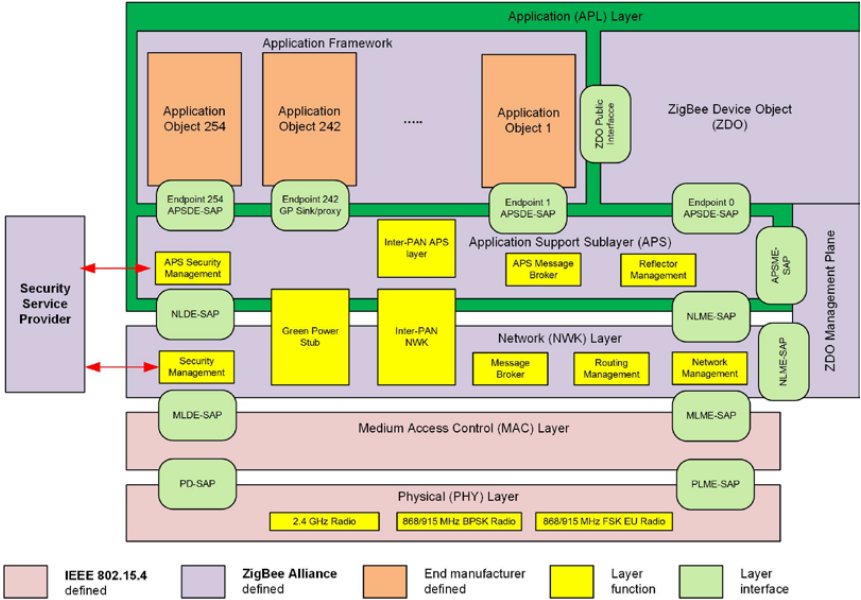
\includegraphics[width=0.99\linewidth]{zigbee_stack_architecture.png}
	\caption{Architektura stosu ZigBee. Źródło:~\cite{zigbee_alliance_zigbee_2017}}
	\label{rys:zigbee_stack_architecture}
\end{figure}

Specyfikacja ZigBee, opierając się na dokumentach IEEE 802.15.4, wykorzystuje częstotliwości
$868/915 MHz$ (w zależności od regionu Europa albo USA/Australia) oraz 2.4GHz~\cite{zigbee_alliance_zigbee_2017}.
Umożliwia tym samym transfer z przepustowością do 250~kbps~\cite{silicon_laboratories_ug10302_2021}.
Omawiany standard wprowadza swoje dodatkowe warstwy komunikacji do stosu: \gls{NWK} oraz~\gls{APL} --
Rysunek~\ref{rys:zigbee_stack_architecture}.
Warstwa aplikacji, będącą najwyższą w~hierarchi, składa się z wielu składowych. \gls{APS} odpowiada za
komunikację pomiędzy \gls{NWK} a~warstwami wyższymi. Oferuje między innymi parowanie urządzeń,
przekazywanie wiadomości, adresację, zajmuje się fragmentacją pakietów i~zapewnia niezawodny transport danych.
\gls{ZDO} w~głównej mierze odpowiada za wyszukiwanie urządzenia i~usług ZigBee~\cite{stmicroelectronics_an5506_2020, zigbee_alliance_zigbee_2017}.
Nadaje on również role urządzeniom sieci.

\begin{figure}[!ht]
	\centering 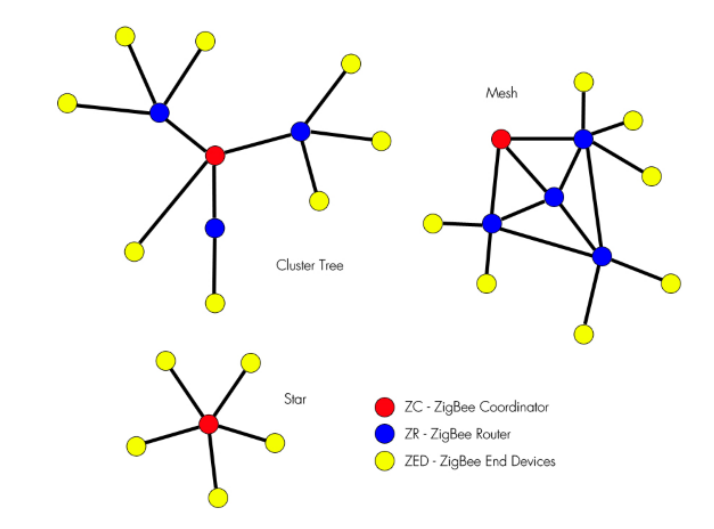
\includegraphics[width=0.618\linewidth]{zigbee_topologies_an5506.png}
	\caption{Topologie sieci ZigBee. Źródło:~\cite{stmicroelectronics_an5506_2020}}
	\label{rys:zigbee_topologies_an5506}
\end{figure}

ZigBee wprowadza trzy główne definicje ról urządzeń rejestrowanych do wewnątrz sieci:
\begin{itemize}
\item \gls{ZC} -- węzeł odpowiadający za utworzenie i~utrzymywanie scentralizowanej sieci, dobór wymaganych parametrów, dodawanie nowych węzłów.
\item \gls{ZR} -- węzeł odpowiadający za przekazywanie danych, który również może przyjąć rolę urządzenia końcowego. 
\item \gls{ZED} -- węzeł końcowy który odbiera i wysyła dane bez możliwości ich routowania.
\end{itemize}

Warstwa sieci umożliwia adaptację trzech rodzajów topologii: gwiazda, drzewo i mesh -- Rysunek~\ref{rys:zigbee_topologies_an5506}.
Typ gwiazdy kontrolowany jest przez jednego koordynatora. Topologia drzewa pozwala zastosować hierarchiczne
sposoby routingu pakietów. Typ mesh z kolei pozwala na pełną komunikację peer-to-peer między węzłami~\cite{zigbee_alliance_zigbee_2017}.
Zestawienie poszczególnych warstw z~modelem referencyjnym OSI znajduje się na Rysunku~\ref{rys:zigbee_osi_comparison_an5506}.

ZigBee umożliwia wykorzystanie następujących metod routingu. Metoda oparta o tablicę trasowania\footnote{z ang. \textit{Routing Table}}
zakłada, iż każdy z~węzłów posiada strukturę przechowującą adresy kolejnych, otaczających go węzłów. Raz wysłana wiadomość,
będzie korzystać z~tej informacji, by przesłać pakiet do miejsca docelowego. W~przypadku niepowodzenia, pierwotny węzeł otrzyma
błąd, by ewentualnie podjąć dalszą decyzję o~ponownym wyznaczeniu trasy. Standard przewiduje wysyłanie również pakietów
przy wykorzystaniu rozgłoszenia z możliwością wyboru roli danego urządzenia. Możliwy jest również multicast. Ostatnią
opcją trasowania jest metoda wiele-do-jednego (źródła)~\cite{silicon_laboratories_ug10302_2021}.

\begin{figure}[!ht]
	\centering 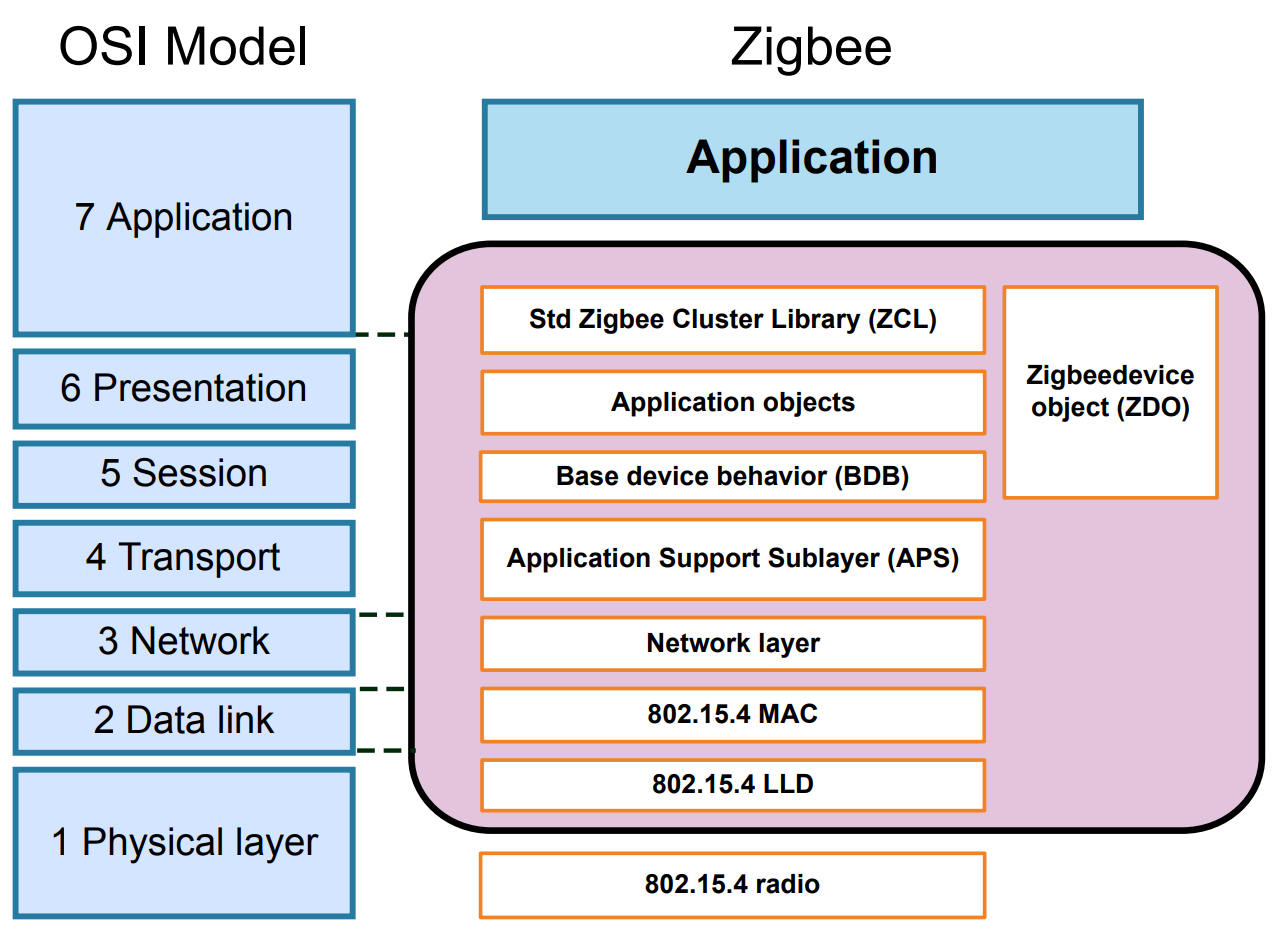
\includegraphics[width=0.618\linewidth]{zigbee_osi_comparison_an5506.png}
	\caption{Zestawienie warstw stosu ZigBee z modelem referencyjnym OSI. Źródło:~\cite{stmicroelectronics_an5506_2020}}
	\label{rys:zigbee_osi_comparison_an5506}
\end{figure}

ZigBee wprowadza termin \textit{profili}, będący kontraktem pomiędzy komunikatami wysyłanymi pomiędzy urządzeniami. Definiuje on
logiczną strukturę danych i zapewniając kompatybilność pomiędzy platformami różnych producentów. Cechą tą charakteryzują
się przede wszystkim profile publiczne zdefiniowane przez ZigBee Alliance. Poszczególni producenci mogą 
również opracować własnościowe, zamknięte struktury do tworzenia wewnętrznych sieci, gdzie kompatybilność pomiędzy
urządzeniami wielu producentów nie jest wymagana~\cite{zigbee_alliance_zigbee_2017, stmicroelectronics_an5506_2020, zigbee_alliance_zigbee_2017}.

\section{Thread}
Thread jest protokół to do zastosowań \gls{IoT} mający swe podstawy w standardzie IEEE 802.15.4.
Umożliwia on tworzenie rozwiązań o niskim zużyciu energii, przy jednoczesnej koncentracji na bezpieczeństwie opierając
adresację o powszechnie znany IPv6. Wybór IPv6 zapewnia płynną integrację z~powszechną infrastrukturą
i~Internetem włącznie. Rozwiązanie jest przez to elastyczne i~mniej podatne na starzenie się technologii.
Same natomiast produkty oparte o~Thread mogą być wdrożone na rynek szybciej dzięki powszechności
internetowych narzędzi deweloperskich. Pierwsza wersja specyfikacji została udostępniona
w 2014 roku i~pozostaje rozwijana do dziś~\cite{noauthor_thread_nodate}.

\begin{figure}[!ht]
	\centering 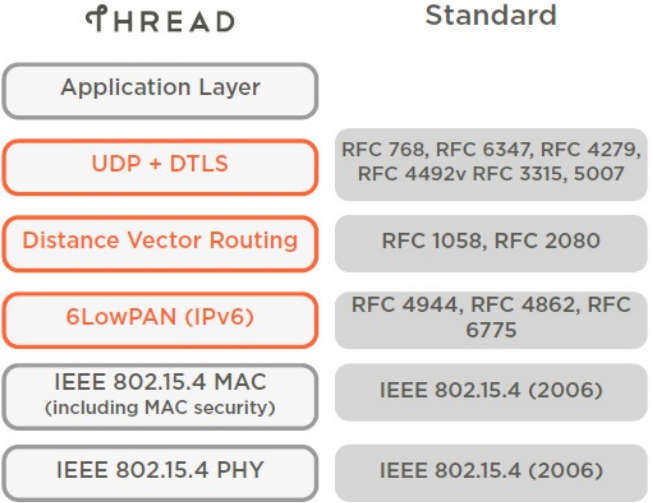
\includegraphics[width=0.618\linewidth]{thread_stack_overview_ug10311.png}
	\caption{Stos Thread i odpowiadające mu specyfikacje RFC/IEEE. Źródło:~\cite{silicon_laboratories_ug10311_2022}}
	\label{rys:thread_stack_overview_ug10311}
\end{figure}

Thread wykorzystuje standard IEEE 802.15.4. Transmisja danych odbywa się na częstotliwości $2.4GHz$ z przepustowością
do 250~kbps. Protokół jest zoptymalizowany do wykorzystywania dużej liczby węzłów wchodzących w skład sieci~\cite{silicon_laboratories_ug10311_2022}.
Celem organizacji sieci w~spójny zbiór fizycznych i~logicznych obiektów, standard wprowadza następującą nomenklaturę.
Rolą węzła typu router jest przekazywanie pakietów w sieci oraz nadzorowanie dostępu do sieci, podczas gdy radio
takiego urządzenia ciągle jest w aktywne. \gls{ED} jest urządzeniem przeważnie komunikującym się z~jednym
routerem będącym jego rodzicem, nie przekazuje pakietów dla innych sieci i~możliwością deaktywacji radia
celem ograniczenia zużycia energii. Dodatkowo, definiuje się następujące typy urządzeń:
\begin{itemize}
\item \gls{FTD} -- urządzenie posiadające ciągle włączone radio, mapujące adresację IPv6
	\begin{itemize}
	\item Router
	\item \gls{REED} -- urządzenie, które można wykorzystywać jako router
	\item \gls{FED} -- urządzenie, którego nie można wykorzystywać jako router
	\end{itemize}
\item \gls{MTD} urządzenie przekazujące komunikaty do rodzica.
	\begin{itemize}
	\item \gls{MED} -- urządzenie, którego radioodbiornik zawsze pozostaje włączony. Nie wymaga periodycznego
	pobierania wiadomości z urządzenia-rodzica
	\item \gls{SED} -- urządzenie wzbudzające radioodbiornik okazjonalnie celem pobrania wiadomości.
	\end{itemize}
\end{itemize}
Standard przewiduje dodatkowe typy jak Thread Leader, będący dynamicznie i automatycznie wybieranym węzłem
zarządzający pozostałymi Router'ami w sieci. Border Router (router brzegowy) służy za bramkę
konwertujący komunikaty przesyłane wewnątrz sieci Thread do sieci zewnętrznych takich jak Internet~\cite{noauthor_node_2022}.

\begin{figure}[!ht]
	\centering 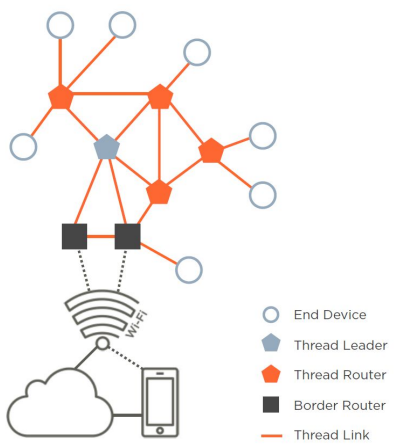
\includegraphics[width=0.618\linewidth]{thread_topology_devices_threadgroup.png}
	\caption{Podstawowa topologia sieci Thread wraz z urządzeniami. Źródło:~\cite{thread_group_thread_2020}}
	\label{rys:thread_topology_devices_threadgroup}
\end{figure}

Dane w sieci przesyłane są w oparciu o~standard \textit{6LoWPAN}\footnote{IPv6 Over Low Power Wireless Personal Networks}.
Protokół ten został zoptymalizowany w ten sposób, by wysyłać maksymalną możliwą ilość danych z użyciem jednego
pakietu celem minimalizacji fragmentacji pakietów, redukując tym samym narzut na CPU i~zużycie energii.
Thread umożliwia stosowanie również protokołów znanych z sieci opartych o model TCP/IP. Tak więc
standard ten obsługuje m.in. \gls{ICMP}, \gls{UDP}, \gls{TCP}. Topologia tym samym również zależy od ilości
węzłów typu router, tworząc albo sieć gwiazdy, albo mesh. Thread obsługuje do 32-óch routerów, gdzie każdy
z~nich może obsłużyć do 511 \gls{ED}. Routing odbywa się na zasadach znanych z~\gls{IP}
wykorzystując w tym celu protokół zbliżony do \gls{RIP}, będący zoptymalizowany do wymagań
IoT pod względem zużycia energii~\cite{silicon_laboratories_ug10311_2022}.

\begin{figure}[!ht]
	\centering 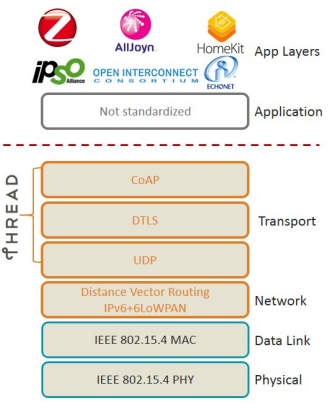
\includegraphics[width=0.618\linewidth]{thread_iso_comparison_ug10311.png}
	\caption{Thread w zestawieniu z modelem OSI. Źródło:~\cite{silicon_laboratories_ug10311_2022}}
	\label{rys:thread_iso_comparison_ug10311}
\end{figure}

Thread będący otwartym standardem może zostać wdrożony przez producenta samodzielnie bądź wybrać stos otwartoźródłowy --~\ref{rys:thread_iso_comparison_ug10311}.
Jednym z takich stosów jest OpenThread\footnote{\url{https://openthread.io/}} będący opracowany przez firmę Google.

Co warto dodać, Thread nie definiuje formatu danych jaki jest wysyłany pomiędzy węzłami. Innymi słowy,
warstwa aplikacji jest nieustandaryzowana~\cite{silicon_laboratories_ug10311_2022}. Obecnie trwają
prace nad opracowaniem wspólnego i~wolnościowego interfejsu. Jednym z takich projektów jest \textit{Matter}\footnote{\url{https://csa-iot.org/all-solutions/matter/}}.

\section{Bluetooth Low Energy}
\lipsum[1-8]

\section{Porównanie przedstawionych standardów} % jako podroździał
% historia jako delikatny wstęp
\url{https://www.silabs.com/documents/public/application-notes/an1142-mesh-network-performance-comparison.pdf}
\url{https://www.silabs.com/wireless/matter}
\lipsum[1-15]


% 1. Krótki rys historyczny standardu
% 2. Opis stosu + jakiś obrazek
% 2.1. Częstotliwości na których pracuej standard
% 3. Topologia, rodzaje węzłów


\chapter{Założenia teoretyczne}
% Zużycie energii - może podłączyć pod rozdział 2.???
*Możliwe, iż ten rozdział nie zostanie rozwinięty*
\section{Zużycie energii}
\cite{noauthor_um1718_2022} jako podstawa dla części teoretycznej. Spróbować symulacji zużycia energii z użyciem PCC w Cube'ie.
Dodatkowo, oprzeć się na literaturze i artykulach naukowych, które poruszają tę kwestię - przynajmniej jeden.

\subsection{Tryb ogłoszeniowy (*komentarz*: model zapożyczony z literatury)}
\subsection{Tryb połączenia (*komentarz*: model zapożyczony z literatury)}

\section{Packet Error Rate}
\subsection{Model zależności PER od odległości i ilości między-węzłów}
\subsection{Wpływ tła radiowego na model (*komentarz*: prezentacja hipotez)}



\chapter{Część doświadczalna}
Treść tego rozdziału przedstawia wszelkie kroki podjęte celem realizacji dwóch
postawionych zadań: badania zużycia energii oraz \gls{PER}. Wprowadzając
czytelnika w~aspekty przygotowawcze eksperymentu i~technikalia z~nimi związane,
przechodzi się do prezentacji wyników i~powiązanych analiz opracowanych wykresów.

Pierwszy podrozdział wprowadza w~aspekty czysto techniczne i~sprzętowe . Uzasadnia wybór
platformy jak i~oprogramowania w~tym \gls{IDE}. Przedstawia się problem
zasilania zestawów uruchomieniowych podczas badań terenowych, jednocześnie prezentując
praktyczne, proste i niskokosztowe rozwiązanie problemów. Ze względu na kruchość
elementów elektronicznych, wprowadza się projekt a następnie omawia
fizyczne wykonanie autorskiej obudowy. Jednakże, głównym elementem tego rozdziału 
jest skoncentrowana na oprogramowaniu. Zarówno oprogramowaniu mikrokontrolerów jak 
i~PC. Przedstawia się wprowadzone funkcjonalności oraz definiuje ich sposób użycia.
Opisuje się kwestię kalibracji uzasadniając potrzebą i~potwierdzając jej skuteczność 
obliczeniami arytmetycznymi bazując na równaniu uzyskanym drogą inżynierii wstecznej.
Ostatnim aspektem poruszanym w tym punkcie jest aplikacja~PC i~jej interfejs
użytkownika.

Drugi podrozdział, prezentuje badanie zużycie energii jako całość. Wprowadza się metodologię
według której dokonano akwizycji danych. Następnie, prezentuje się wykresy podając opis
do każdego z nich. Badania oparto o dwa główne aspekty -- konsumpcja energii przez
przez usługę BLE \gls{HRT} oraz model BLE Mesh. Ostatecznie, zestawia się zebrane
w~ten sposób dane.

Ostatni podrozdział dotyczy eksperymentu PER. Analogicznie do wyżej wymienionego
doświadczenia, wprowadza metodologię badań oraz określa kategorię zbieranych zmiennych
i~definiuje się parametry stałe transmisji. Zebrane dane w próbach terenowych następnie
są dzielone na dwie kategorie: PER względem częstości zapytań oraz PER względem
odległości między węzłami. Wyniki, w postaci szeregu wykresów, są następnie
omawiane.

%%!!!!!!!!!!!!!!!!!!!!!!!!!!!!!!!!!!!!!!!!!!!!!!!!!!!!!!!!!!!!!!!!!!!!!!!!!!!!!!
%%%%%%%%%%%%%%%%%%%%%%%%%%%%%%%%%%%%%%%%%%%%%%%%%%%%%%%%%%%%%%%%%%%%%%%%%%%%%%%%
%% SECTION: Przygotowanie eksperymentu
%%%%%%%%%%%%%%%%%%%%%%%%%%%%%%%%%%%%%%%%%%%%%%%%%%%%%%%%%%%%%%%%%%%%%%%%%%%%%%%%
%%!!!!!!!!!!!!!!!!!!!!!!!!!!!!!!!!!!!!!!!!!!!!!!!!!!!!!!!!!!!!!!!!!!!!!!!!!!!!!!
\section{Przygotowanie eksperymentu}

Eksperymentalna część pracy bezsprzecznie wymaga przygotowania odpowiedniego zestawu
sprzętu i~narzędzi. Konieczne jest wybranie odpowiedniej platformy sprzętowej
wspierającej komunikację bezprzewodową Bluetooth Low Energy w wersji minimum 5.0.
Niezbędne jest również oprzyrządowanie pomiarowe, które umożliwia pomiar natężeń
prądu poniżej 1mA, ze względu na energooszczędność urządzeń \gls{BLE}.

% zakładam, że we wcześniejszych rozdziałach definiuję zakres pracy i rodzaje eksperymentów

Badania zużycia energii wymagają aparatury, która w pełni zarejestruje minima i maksima
poboru prądu przy niskich błędach pomiarowych. Na podstawie otrzymanych danych wykonane zostaną
właściwe obliczenia ukazujące zużycie energii przez urządzenie dla wielu trybów działania.

Eksperyment \gls{PER} wymaga przygotowania wielu zestawów uruchomieniowych obsługujących
komunikację BLE w konfiguracji Mesh. Dodatkowo, wymagane jest stworzenie dedykowanego oprogramowania
na mikrokontroler jak i komputer osobisty. Jest to niezbędne w celu kontroli przepływu
doświadczenia jak i akwizycji danych.

Niniejszy rozdział omawia zakres poniesionych przygotowań do przeprowadzenia 
właściwych eksperymentów.


%%%%%%%%%%%%%%%%%%%%%%%%%%%%%%%%%%%%%%%%%%%%%%%%%%%%%%%%%%%%%%%%%%%%%%%%%%%%%%%%
%% SUBSECTION: Sprzęt i oprzyrządowanie
%%%%%%%%%%%%%%%%%%%%%%%%%%%%%%%%%%%%%%%%%%%%%%%%%%%%%%%%%%%%%%%%%%%%%%%%%%%%%%%%
\subsection{Sprzęt i oprzyrządowanie}

% nie pisać i tłumaczyć własnych preferencji. Raczej pisać generyczny bullshit

Próby doświadczalne oparto o produkty firmy STMicroelectronics (krócej: ST). Jest to europejska firma
obejmująca swym portfolio projektowanie i produkcję elementów elektronicznych. Jedną
z~ich linii produktów są 32-bitowe mikrokontrolery architektury ARM, znane również jako STM32.
Są to rozwiązania cenione na rynku.

Ze względu na powszechność stosowanych rozwiązań, jednak nie ograniczając się wyłącznie do tego kryterium,
wybrano mikrokontroler z rodziny STM32WB. Gotowe, komercyjnie dostępne zestawy ewaluacyjne oraz
zintegrowany ekosystem stanowią doskonałą podstawę dla badań Bluetooth Low Energy.


\subsubsection{P-NUCLEO-WB55}

Badania Bluetooth Low Energy wymagały wyboru platformy, która umożliwia eksperymentalną 
weryfikację wybranych celów badawczych. Ostatecznie, zdecydowano się na wykorzystanie 
mikrokontrolera \textit{STM32WB55RG}. W celu zapewnienia powtarzalności eksperymentu jak 
i~ze względu na ograniczenia czasowe, docelową platformą badawczą stał się zestaw 
uruchomieniowy \textit{P-NUCLEO-WB55}~\cite{noauthor_p-nucleo-wb55_nodate}.

\begin{figure}[!htb]
	\centering 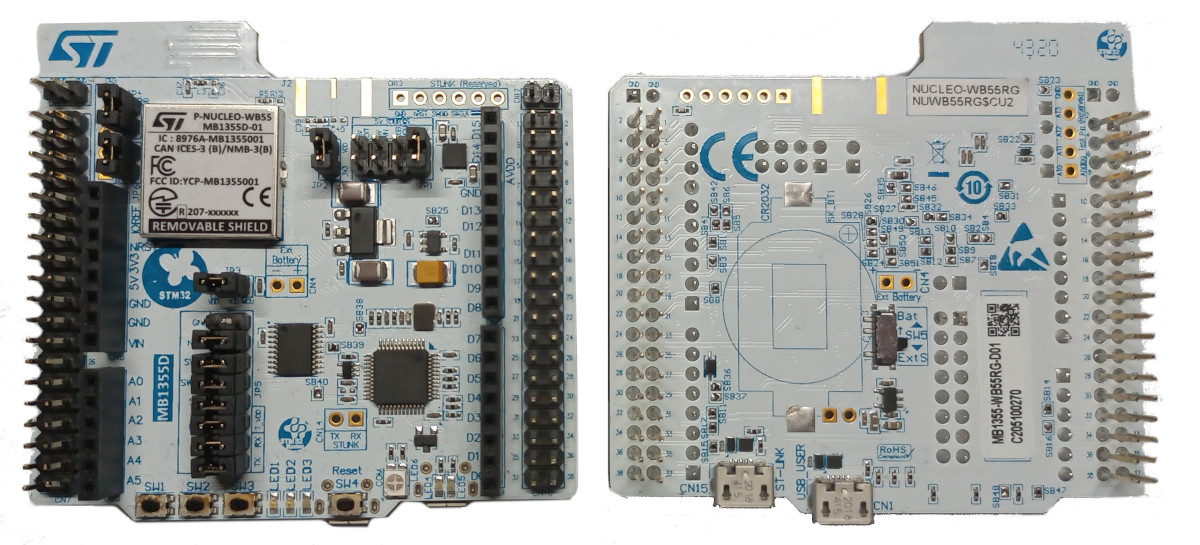
\includegraphics[width=0.618\linewidth]{nucleo_wb55.jpg}
	\caption{Zestaw uruchomieniowy P-NUCLEO-WB55}
	\label{rys:nucleo_wb55}
\end{figure}

Zestaw ten zgodny jest ze specyfikacją Bluetooth Low Energy v5.0. Dodatkowo, wspiera
on inne standardy komunikacji, m.in. Zigbee~\cite{noauthor_stm32wb_2022}.
Ten fakt może zostać wykorzystany w celu bezpośredniego porównania różnych stosów komunikacji bezprzewodowej.
Nie jest to jednak celem niniejszej pracy, a stanowi możliwość jej dalszego 
rozwinięcia.


\subsubsection{X-NUCLEO-LPM01A} \label{device:plytka_pomiarowa}

Płytka rozszerzeń X-NUCLEO-LPM01A spełnia wszelkie oczekiwania dotyczące możliwości pomiarowych
stawianych przed projektem. Wg oficjalnej dokumentacji \cite{noauthor_um2243_2018}, układ oferuje:

\begin{itemize}
\item Programowalne źródło napięciowe 1,8V do 3,3V
\item Dynamiczne próbkowanie w zakresie od 100nA 50mA przy maksymalnej częstotliwości 100kHz z 2\%-ową dokładnością pomiarów
\item Pomiar statyczny natężenia prądu do 200mA
\item Integracja z aplikacją do dedykowaną aplikacją akwizycji danych \cite{noauthor_stm32cubemonpwr_2022}
\end{itemize}

\begin{figure}[!ht]
	\centering 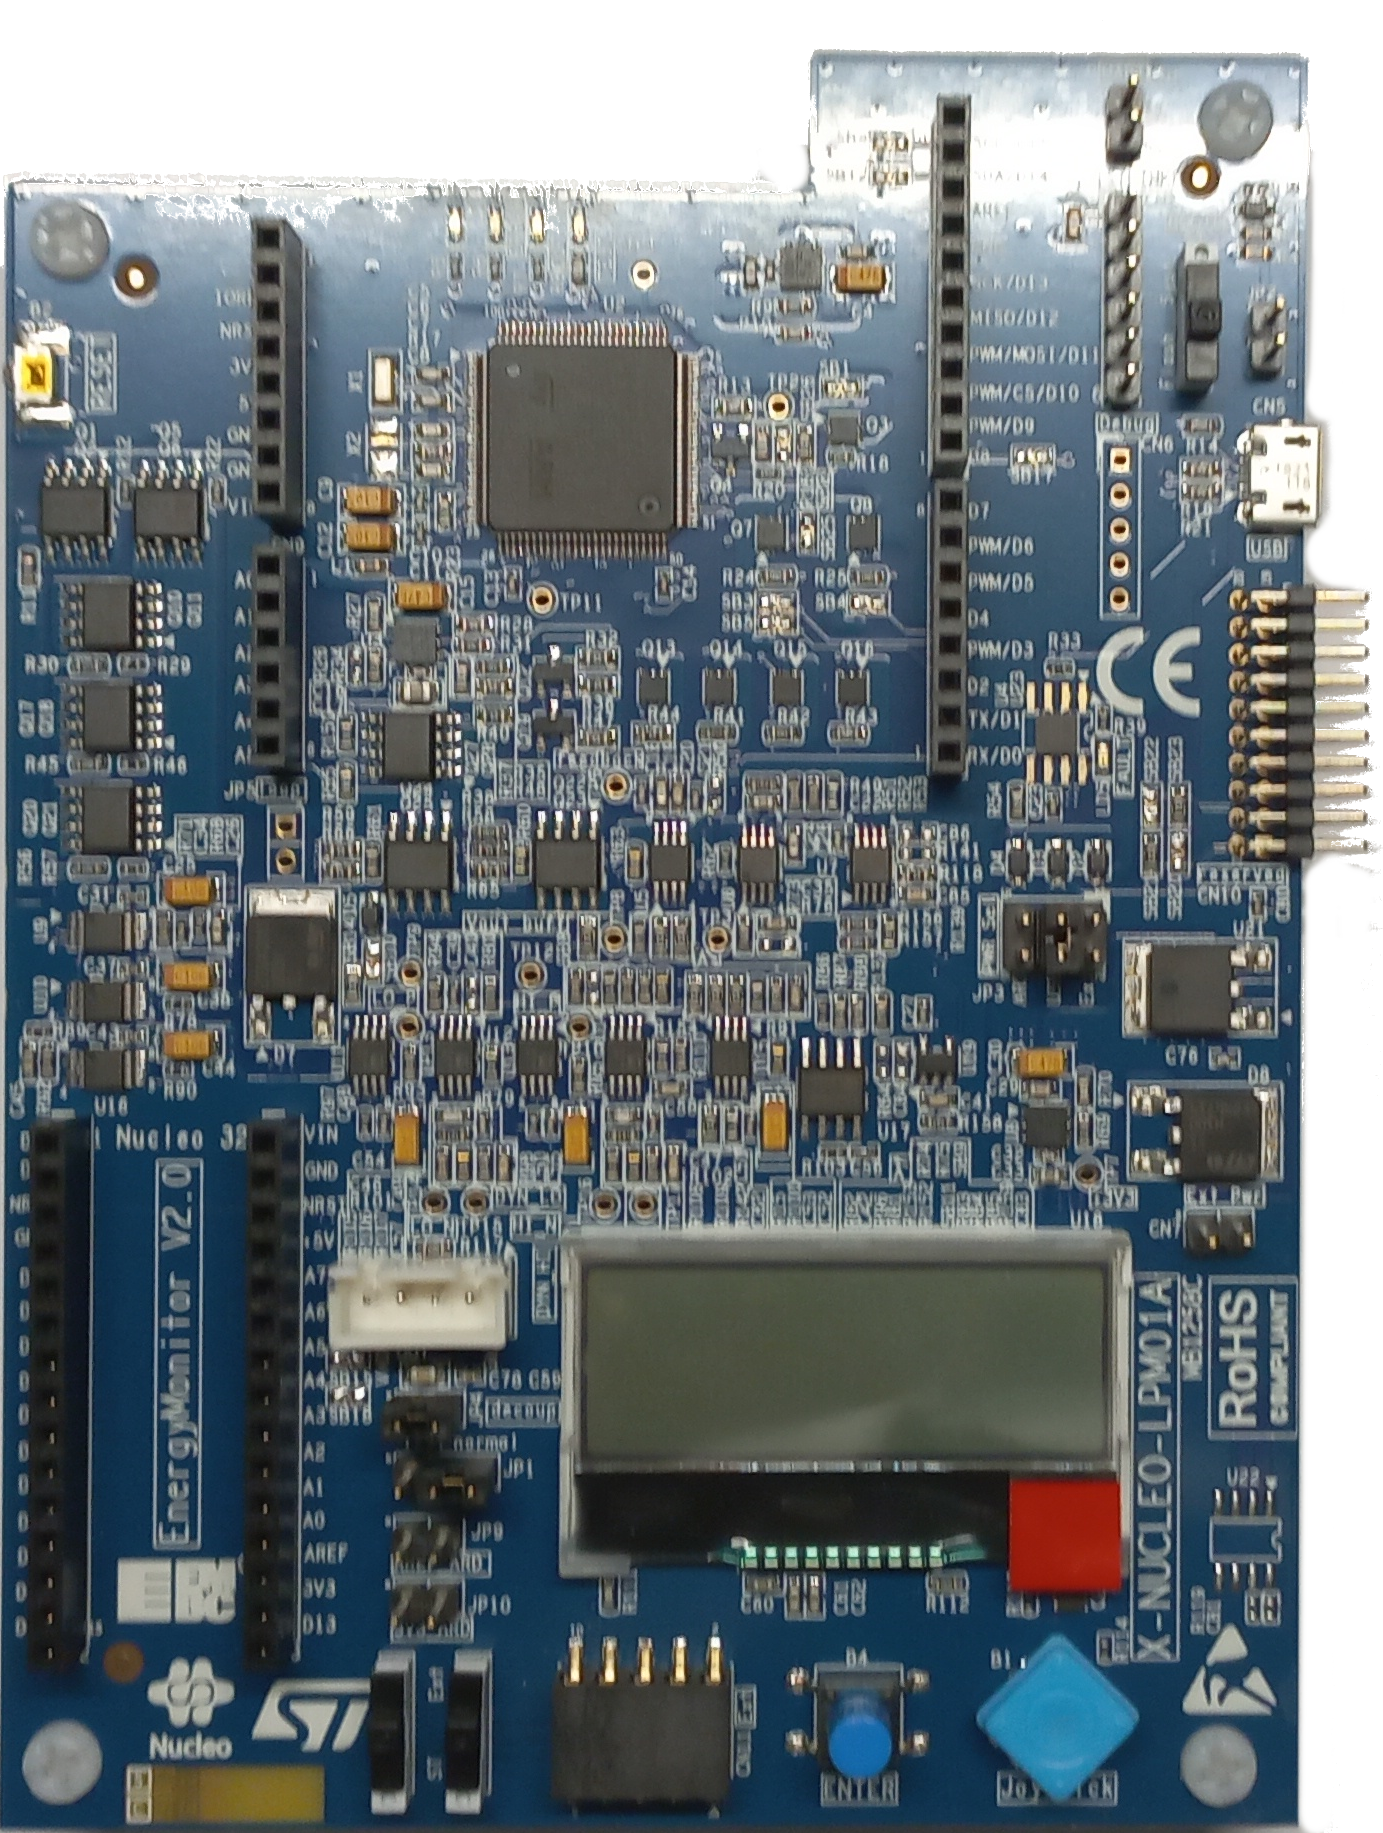
\includegraphics[width=0.618\linewidth]{st_power_measurement_unit.png}
	\caption{Zestaw pomiarowy X-NUCLEO-LPM01A}
	\label{rys:nucleo_lpm01a}
\end{figure}

Moduł ten nie ogranicza się tylko do wykorzystywania autorskich złącz firmy ST. Schemat wyprowadzeń pinów
umożliwia wykorzystanie popularnych platform takich jak Arduino\footnote{https://www.arduino.cc/}. Co istotniejsze, wybrana płytka umożliwia
zasilanie dowolnego układu dzięki wyprowadzeniu źródła napięciowego za pośrednictwem pinów 
(za dokumentacją: złącze CN14). Ten fakt został wykorzystany w badaniach, pozwalając uniknąć kłopotliwej
konfiguracji P-NUCLEO-WB55 wymagającej tworzenia dodatkowych ścieżek lutowanych.

Dodatkową cechą tego modułu jest akwizycja danych z użyciem komputera osobistego. Dzięki dedykowanej
aplikacji, dostarczanej wraz z modułem, możliwa jest akwizycja danych w czasie rzeczywistym przy
wybranych częstotliwościach próbkowania. Zebrane w ten sposób dane służą dalszym analizom, co zostało
wykorzystane w niniejszej pracy. 

\subsubsection{Narzędzia i firmware firmy ST}
Firma ST wraz z zestawem uruchomieniowym udostępnia pełne zintegrowane środowisko
programistyczne oraz niezbędne biblioteki i certyfikowany firmware:

\begin{itemize}
\item \textbf{STM32CubeIDE} \cite{noauthor_stm32cubeide_2022} -- multiplatformowe zintegrowane środowisko programistyczne
dostarczane przez ST bazujące na otwartoźródłowym środowisko \textit{Eclipse}\footnote{https://www.eclipse.org/ide/}.
\item \textbf{STM32CubeProgrammer} \cite{noauthor_stm32cubeprog_2022} -- narzędzie umożliwiające wykonywanie operacji
odczytu, zapisu i weryfikacji skompilowanego oprogramowania produktów STM32. 
\item \textbf{STM32CubeMonitor-Power} \cite{noauthor_stm32cubemonpwr_2022} -- oprogramowanie służące akwizycji danych
pod postacią chwilowego poboru prądu elektrycznego m.in. w zestawie X-NUCLEO-LPM01A Rysunek: \ref{rys:nucleo_lpm01a}.
\item \textbf{Firmware STM32CubeWB} \cite{noauthor_stm32cubewb_2022} -- zestaw bibliotek, narzędzi oraz przykładów
przeznaczonych dla mikrokontrolerów rodziny STM32WB. W skład tego repozytorium wchodzą zależności takie jak:
skompilowany, zamknięty firmware ko-processora dla różnych stosów połączeń bezprzewodowych; przykłady programów
wykorzystujące biblioteki HAL jak i również bezpośrednio rejestry; przykłady BLE; przykłady BLE Mesh.
\end{itemize}

%%%%%%%%%%%%%%%%%%%%%%%%%%%%%%%%%%%%%%%%%%%%%%%%%%%%%%%%%%%%%%%%%%%%%%%%%%%%%%%%
%% SUBSECTION: Zasilanie i obudowy
%%%%%%%%%%%%%%%%%%%%%%%%%%%%%%%%%%%%%%%%%%%%%%%%%%%%%%%%%%%%%%%%%%%%%%%%%%%%%%%%
\subsection{Narzędzia i elementy dodatkowe}

\subsubsection{Zasilanie}
Próby terenowe wymagają odrębnego, właściwego zasilania. Wybrane zestawy uruchomieniowe
wykorzystują ustandaryzowane złącze komunikacyjne USB. Złącze to oprócz komunikacji
oferuje zasilanie linią +5V. Przeprowadzając właściwe eksperymenty wykorzystano
komercyjnie dostępne banki energii tzw. powerbanki. Są to akumulatory litowo-jonowe
lub litowo-polimerowe z wbudowanym systemem zarządzania baterią\footnote{\gls{BMS} -- ang. Battery Management System}
i~właściwymi przetwornicami impulsowymi w celu zapewnienia odpowiedniego napięcia zasilania.

Elektronika wbudowana w~magazyny energii automatycznie wyłącza zasilanie w przypadku braku
podłączonego urządzenia lub gdy dane urządzenie pobiera marginalnie niskie wartości
prądu. Służy to ochronie cennego i delikatnego akumulatora. Jest to cecha korzystna
z punktu widzenia konsumenta kupującego powerbank w celu szybkiego ładowania urządzeń elektronicznych.
Niestety, zaleta ta staje się wadą w przypadku przeprowadzanych doświadczeń. Podłączając moduł P-NUCLEO-WB55,
urządzenie po pewnym okresie działania wyłącza się na skutek uruchomionych zabezpieczeń w źródle energii.

W celu przeciwdziałania temu zjawisku, skonstruowano trywialne urządzenie, które wlutowane równolegle w linię zasilania 5V,
konsumuje ok. 100mA prądu: $0,5W = 5V \cdot 0,02A \cdot 5 [diod]$. Doświadczalnie stwierdzono, że tak włączony
odbiornik energii umożliwia stabilne działanie włączonego do sieci modułu STM32. Schemat 
zaprezentowano na Rysunku~\ref{rys:power_led_consumer}

\begin{figure}[!ht]
	\centering 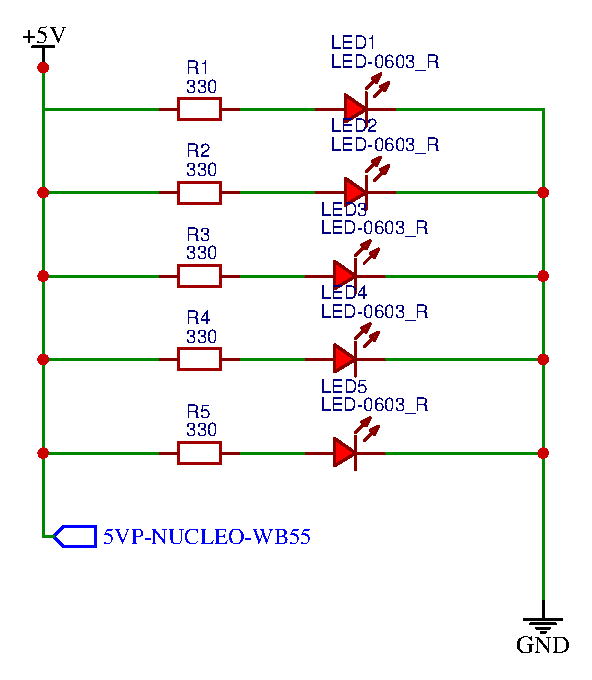
\includegraphics[width=0.618\linewidth]{power_led_consumer.pdf}
	\caption{Odbiornik energii}
	\label{rys:power_led_consumer}
\end{figure}

\subsubsection{Obudowa -- druk 3D}
Kolejnym elementem niezbędnym w celu przeprowadzenia eksperymentów terenowych jest zapewnienie
ochrony mechanicznej wybranych zestawów uruchomieniowych. Podczas prób, elementy mogą zostać
fizycznie uszkodzone poprzez m.in. wyłamanie fragmentu \gls{PCB} (w~tym anteny), uszkodzenie pinów etc.

Wykorzystując techniki projektowania wspomaganego komputerowo\footnote{\gls{CAD} -- ang. \textit{Computer-aided Design}},
zaprojektowano autorską obudowę. Głównym celem projektowym było zapewnienie minimalnej ochrony
mechanicznej, jednocześnie redukując możliwy wpływ materiału na tłumienie sygnału. Elementy
interfejsu: przyciski i~antena, zostały celowo wyeksponowane. Rzut izometryczny przedstawiony został
na Rysunku~\ref{rys:obudowa_model3d}.


\begin{figure}[!htb]
	\centering 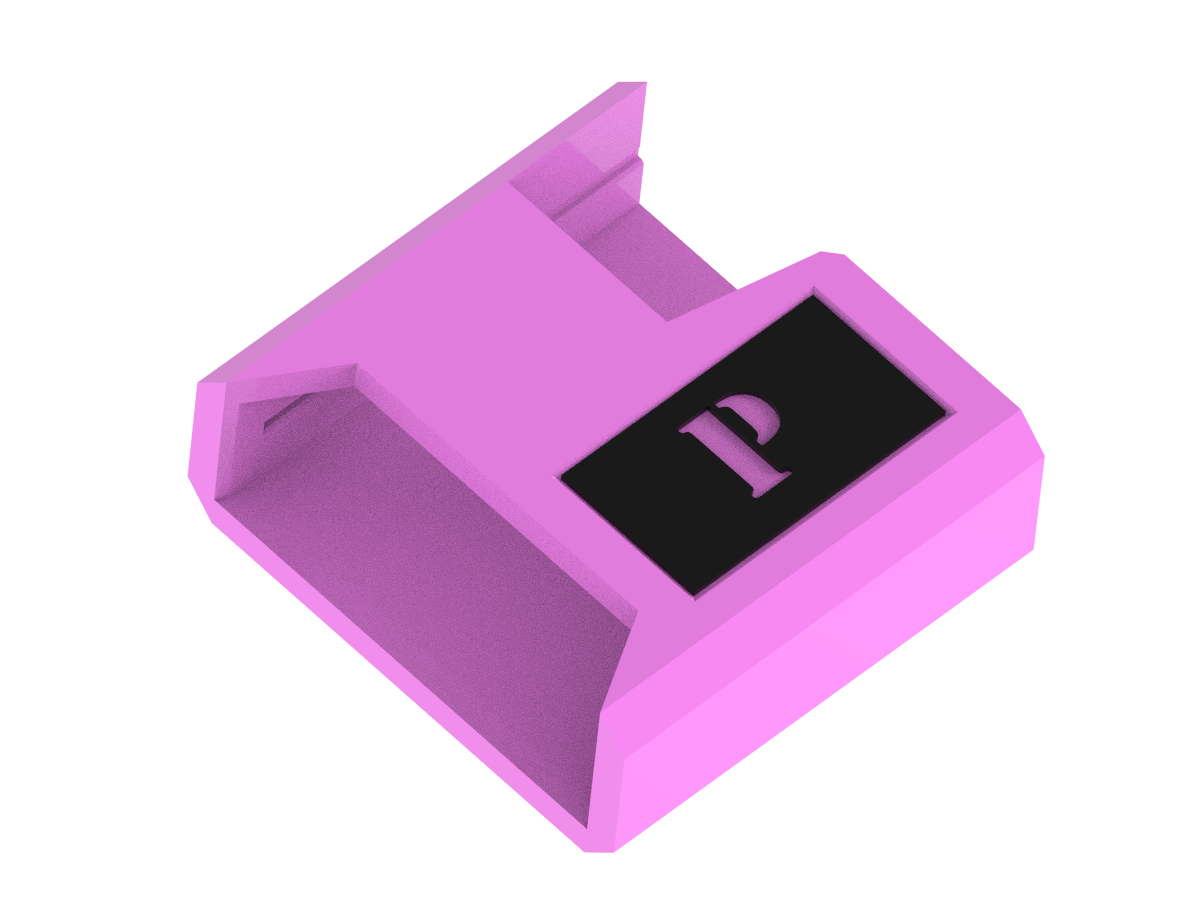
\includegraphics[width=0.618\linewidth]{stm_case_render.png}
	\caption{Model obudowy dla zestawu P-NUCLEO-WB55}
	\label{rys:obudowa_model3d}
\end{figure}

Obudowa wykonana została z materiału \gls{PLA}\footnote{PLA -- ang. \textit{Polylactic acid}, polilaktyd} techniką
druku 3D \gls{FDM}\footnote{FDM -- ang. \textit{Fused Deposition Modeling}}/\gls{FFF}\footnote{FFF -- \textit{Fused Filament Fabrication}}.
Jednobryłowa konstrukcja podyktowana została chęcią uproszczenia wydruku, kosztem zwiększonych trudności
doboru tolerancji dla umieszczanych wewnątrz płytek \gls{PCB}. Obudowa przewiduje wsuwanie modułu Nucleo
do wewnątrz, zapewniając jednoczesne pewne jego mocowanie.

Dobór koloru wydruku również nie był przypadkowy. Przewidując potencjalne lokalizacje przeprowadzanych
doświadczeń, wybrano kolor możliwie jaskrawy. Podstawowym założeniem było ułatwienie dostrzeżenia
obudowy, a wraz z obudową również zestawu uruchomieniowego, pośród flory leśnej czy terenów
zurbanizowanych. Ostateczne wykonanie obudów zaprezentowano na Rysunku~\ref{rys:obudowa_wykonanie}.

\begin{figure}[!htb]
	\centering 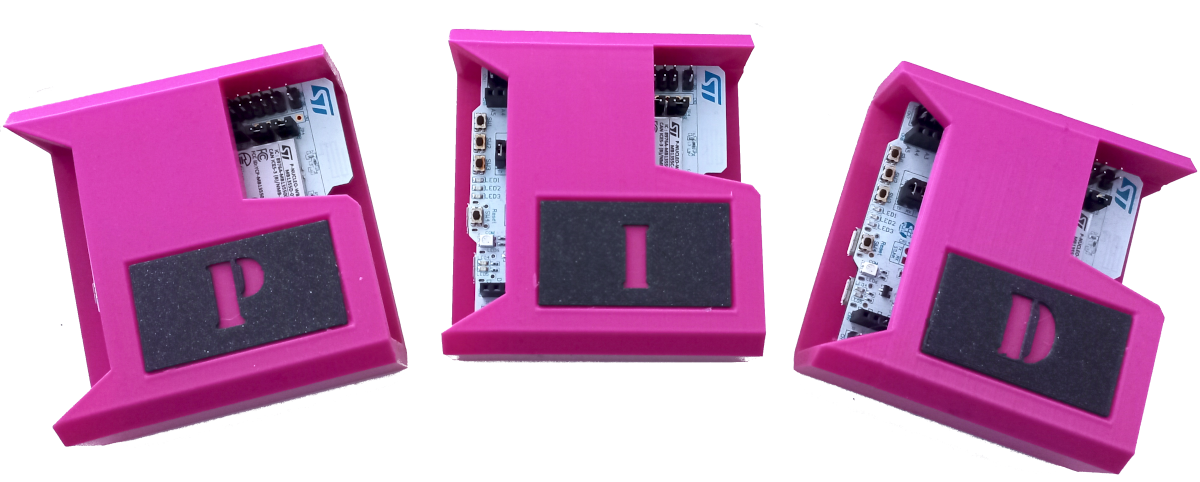
\includegraphics[width=0.618\linewidth]{3d_real_cases.png}
	\caption{Obudowa zestawu uruchomieniowego Nucleo wykonana w technologii druku 3D -- realizacja}
	\label{rys:obudowa_wykonanie}
\end{figure}

%%%%%%%%%%%%%%%%%%%%%%%%%%%%%%%%%%%%%%%%%%%%%%%%%%%%%%%%%%%%%%%%%%%%%%%%%%%%%%%%
%% SUBSECTION: Oprogramowanie mikrokontrolera
%%%%%%%%%%%%%%%%%%%%%%%%%%%%%%%%%%%%%%%%%%%%%%%%%%%%%%%%%%%%%%%%%%%%%%%%%%%%%%%%
\subsection{Oprogramowanie mikrokontrolera} \label{prep:uc-software}

Oczywistym faktem jest, iż zdefiniowane wcześniej rodzaje eksperymentów wymagają
odpowiedniego oprogramowania. Zarówno oprogramowania dla mikrokontrolera
jak i~komputera PC pozwalającego wykonać i~nadzorować wybrane doświadczenia.
Podrozdział ten prezentuje kroki podjęte w celu stworzenia odpowiednich
programów dla badania poboru zużycia energii i~utraty pakietów podczas
transmisji danych.

Pierwszym krokiem jest wybór odpowiedniego zestawu narzędzi i~frameworka,
na którym oparte będą wszelkie dalsze pracy. Rozpatrywane były dwa odrębne
stosy technologiczne: Zephyr OS\footnote{\url{https://www.zephyrproject.org/}} i~natywny dostarczany przez \textit{ST}.
Zephyr OS, będący systemem operacyjnym czasu rzeczywistego (\textit{RTOS}), jest kompletnym zestawem
narzędzi i metodologii wytwarzania oprogramowania dla mikrokontrolerów różnych producentów. Możliwość
przeniesienia kodu na inną platformę z minimalną ilością modyfikacją było opcją nadzwyczaj interesującą.
Jednakże, pomimo oficjalnego wsparcia mikrokontrolera STM32WB55, nie udało się poprawnie
zainstalować dostarczanych przykładów na urządzeniu w sposób umożliwiający ich działanie. Stąd zaniechano
dalszych prób wykorzystania tego systemu operacyjnego w projekcie.

Drugim oczywistym kandydatem jest stos oprogramowania dostarczony przez ST. Jest to niejako
domyślny wybór. Wybrano więc stos oprogramowania dla mikronkontrolera w wersji v1.13.2, jako
najnowszy dostępny w chwili rozpoczęcia prac. Zestaw bibliotek i~narzędzi dostarczanych
przez producenta został wcześniej przez niego przetestowany dając niejako gwarancję spełnienia 
minimalnych standardów umożliwiających m.in. certyfikację urządzenia jako wspierającego
BLE i~BLE Mesh.

Badanie zużycia energii (\ref{experiment:energy-consumption}), wykorzystuje dostarczaną wraz ze stosem przykładową aplikację 
opracowaną przez producenta mikrokontrolera. Owa aplikacja, BLE \gls{HRT}, wykorzystuje zdefiniowany
przez Bluetooth SIG profil \textit{HeartRate} publikując regularnie, co sekundę
odpowiednią wiadomość odbieraną przez odbiornik -- telefon/tablet. Do badań
konsumpcji wykorzystano niezmodyfikowany przykład.

Doświadczenie \gls{PER} wymaga bardziej wyrafinowanego podejścia, zdefiniowanego z wymaganiami
metodologii w punkcie~\ref{subsubsec:test-procedure}. Jako podstawę dla kolekcji trzech aplikacji
wybrano przykład \texttt{BLE\_MeshLightingPRFNode}. Przykład ten wprowadza bezpośrednio
w~pełny stos BLE Mesh umożliwiając jednocześnie wdrożenie pożądanych modeli Mesh jak
i~przypisanie węzłom konkretnej funkcji w sieci: Proxy, Relay, Friend \cite{st_an5292_2021}.

Badając właściwości sieci, wprowadza się następujące nazewnictwo węzłów celem łatwiejszej identyfikacji:
\begin{itemize}\label{node-naming-convention}
	\item węzeł bliższy (ang. \textit{proximal node}) -- węzeł będący połączony bezpośrednio
	ze stacją akwizycji danych i kontroli przepływu eksperymentu. Dodatkowo, węzeł ten udostępnia tryb \textit{Proxy}\footnote{z ang. pośrednik -- tryb umożliwiający dostęp do sieci Mesh urządzeniom poprzez odpowiadającą usługę BLE. Umożliwia
	on m.in. dostęp do sieci i zarządzania nią z poziomu urządzenia nie posiadającego ani nie wspierającego bezpośrednio stos BLE Mesh}
	\item węzeł środkowy (ang. \textit{intermedial node}) -- węzeł działający w trybie
	przekaźnika (terminologia Mesh: \textit{Relay}). Węzeł ten nie uczestniczy bezpośrednio w badaniach tj. nie są
	z niego odczytywane jakiekolwiek dane.
	\item węzeł dalszy (ang. \textit{distal node}) -- węzeł zliczający ilość odebranych danych \textit{r},
	udostępniający jednocześnie usługę umożliwiającą odczyt tych wartości. 
\end{itemize}

Posiadając trzy węzły, wymagane jest również dostarczenie trzech zestawów oprogramowania dla każdego z nich, w zależności
od pełnionej funkcji.

\subsubsection{Węzeł bliższy}\label{sec:proximal-node}
Pierwszy węzeł, węzeł bliższy, odpowiada bezpośrednio za przeprowadzany eksperyment. Jego celem jest wysyłanie właściwych
pakietów do węzła dalszego w~określonych interwałach czasowych. Dodatkowo, służy jako bramka do odbioru liczby mówiącej
o całkowitej ilości odebranych pakietów. Trzecim zadaniem tego modułu jest zresetowanie licznika z każdą nową iteracją
badania PER.

\begin{lstlisting}[language=C,
    caption={Kod uruchamiający sekwencję badawczą PER},
    label={lst:code_generic_onoff}]
// plik: appli_test.c
MOBLE_RESULT Test_ApplicationTest_Set05_GenericOnOff(MOBLE_ADDRESS src ,MOBLE_ADDRESS dst)
{
	MOBLE_RESULT result = MOBLE_RESULT_SUCCESS;
	// [...]
	meshTest.name = OP_NAME_SET05;
	meshTest.counter = 0;
	result = test_set05_generic_initialize(src, dst);
	if (!result)
	{
		run_timer(OP_NAME_SET05, test_generic_subscription, src, dst, test_set05_generic);
		result = MOBLE_RESULT_SUCCESS;
	}
	else
	{
		TRACE_I(TF_VENDOR_M,"%s Could not initialize the test due to error code=%d \r\n", OP_NAME_SET05, result);
		result = MOBLE_RESULT_FAIL;
	} // [...]

	return result;
}
\end{lstlisting}

Listing~\ref{lst:code_generic_onoff} przedstawia kod uruchamiający sekwencję badawczą PER. Linie 4-6 inicjalizują niezbędne
parametry m.in. identyfikujące aktualnie uruchomione doświadczenie. Przypisywana jest wartość zero do licznika inkrementującego
ilość wysłanych pakietów. Jest to o tyle  konieczne, iż pozwala na bezpośrednie porównanie ilości wysłanych komunikatów do
ilości odebranych w innym węźle. Linia 8 odpowiada ze wyzerowanie licznika po stronie węzła dalszego. Wysyłany jest odpowiedni
komunikat wykorzystujący model Vendor'a z id \texttt{APPLI\_TEST\_CMD}. W treści wiadomości wysyłana jest odpowiednia wartość numeryczna
interpretowana przez węzeł dalszy polecenie zresetowania węzła: \texttt{APPLI\_TEST\_PACKET\_ERROR\_RATE\_COUNTER=0x09U}, jak
pokazano na listingu~\ref{lst:code-distal-code-reset}.
W~przypadku, w~którym zresetowanie licznika się powiedzie, dalsza część funkcji przystępuje do uruchomienia timer'a
w linii 11.

\begin{lstlisting}[language=C,
    caption={Kod resetujący wartość licznika w węźle dystalnym},
    label={lst:code-distal-code-reset}]
// plik: appli_test.c
MOBLE_RESULT test_set05_generic_initialize(MOBLE_ADDRESS src ,MOBLE_ADDRESS dst)
{
	MOBLE_RESULT result = MOBLE_RESULT_SUCCESS;
	AppliBuffer[0] = APPLI_TEST_PACKET_ERROR_RATE_COUNTER;

	result = BLEMesh_SetRemotePublication(VENDORMODEL_STMICRO_ID1, src,
	APPLI_TEST_CMD,
	AppliBuffer, sizeof(AppliBuffer),
	MOBLE_TRUE, MOBLE_TRUE);

	if (result)
	{
		TRACE_I(TF_VENDOR_M, "%s Could not initialize the test due to error code=%d \r\n", OP_NAME_SET05, result);
	}
	return result;
}
\end{lstlisting}

Dodatkową uwagę zwrócić na nazewnictwo samych funkcji. Wskazują one numer polecenia (\texttt{Set05}, \texttt{Set06}). Numer ten wykorzystywany
jest przez \textit{Mesh Serial Gateway} i~interpretowany w sposób umożliwiający uruchomienie opisywanej funkcji. 
Nie jest to ścisłe wymaganie a raczej konwencja, kontrakt wprowadzony przez ST dla danego pliku. Niemniej jednak, pozwala
ona w jasny i~czytelny sposób zidentyfikować polecenie i odpowiadające polecenie \gls{AT} (zbliżone do poleceń AT). Opis
działania interfejsu PC-STM32WB55 znajduje się poniżej \ref{mesh:serial-gateway}.

\subsubsection{Timer}\label{sec:timer}
Timer odpowiada za regularne wykonywanie zdefiniowanej funkcji. Odpowiada on za główny przepływ 
badania interpretując zebrane parametry doświadczenia i~je wykonując. Kod oparto o interfejs programistyczny
dostarczony przez ST~\cite{stmicroelectronics_an5289_2021}\footnote{rozdział \textit{4.5 Timer server}}.

\begin{lstlisting}[language=C,
    caption={Funkcja aktywująca timer},
    label={lst:timer_activation_function}]
// plik: appli_test.c; Usunieto linie logujace przeplyw TRACE_I
static void run_timer(char const *setName, MeshTest_t subscriptionType, MOBLE_ADDRESS src ,MOBLE_ADDRESS dst, void (*callback)(void) ) {
	MOBLEUINT16 triggerInterval;
	MOBLEUINT32 killAfterTimeout;

	triggerInterval = timerTriggerInterval;
	killAfterTimeout = Totaltest;

	HW_TS_Create(subscriptionType, &(meshTest.timer_subscription_id), hw_ts_Repeated, callback);
	HW_TS_Create(test_kill_subscription, &(meshTest.timer_kill_subscription_id), hw_ts_SingleShot, kill_subscription);

	meshTest.startTimestamp = HAL_GetTick();
	HW_TS_Start(meshTest.timer_subscription_id, triggerInterval);
	HW_TS_Start(meshTest.timer_kill_subscription_id, killAfterTimeout);
}
\end{lstlisting}

Listing~\ref{lst:timer_activation_function} przedstawia wdrożony kod uruchamiający timer. Najistotniejszym parametrem funkcji jest
wskaźnik do funkcji umożliwiający uruchomienie kodu w odpowiedzi na zdarzenie (\textit{callback}). Linie 6-7 przypisują
wartości kolejno interwału, z którym periodycznie ma być uruchamiany \textit{callback} oraz wartość po której upłynięciu
timer zostanie wyłączone. Obie te zmienne są typu logicznego \textit{tick}. Podawane w~nich są wartości ticków procesora aniżeli
milisekundy. Przed przypisaniem wartości należy przekonwertować milisekundy do ticków w~zależności od konfiguracji
zegara RTC mikrokontrolera. Zagadnienie to stanowiło problem na etapie tworzenia procedury badawczej. Ostatecznie zdecydowano
się na wprowadzenie pojęcia kalibracji, w której to wyznaczano eksperymentalnie wartości ticków względem oczekiwanej długości
okresu czasu. Logika takiego procesu opisana została w~punkcie dotyczącym oprogramowania PC~\ref{prep:pc-software}.

Linie 9-10, rejestrują wybrane funkcje (poprzez wskaźniki do funkcji) do wewnątrz silnika timera dostarczanego przez ST.
Linijki 12-13 kolejno uruchamiają timer. Dzięki temu wprowadzono substytut wielowątkowości wykonując wiele procesów (tutaj: funkcji)
pozornie jednocześnie bądź w ustalonej sekwencji. Rezultatem działania tego kodu jest periodyczne uruchamianie
funkcji \textit{callback} oraz jej zamknięcie po ustalonym czasie.

Opierając się na inżynierii wstecznej, znaleziono współczynnik, przeliczający wartości milisekund do ticków:

\begin{lstlisting}[language=C,
    caption={Ścieżka inżynierii wstecznej w celu znalezienia współczynnika umożliwiającego konwersję milisekund do ticków},
    label={lst:millis-to-tick-reverse-engineering}]
// plik: stm32wbxx_hal_conf.h
#define LSE_VALUE  ((uint32_t)32768) /*!< Value of the External oscillator in Hz*/

// plik app_common.h
#define DIVR( x, y )  (((x)+((y)/2))/(y))

// plik app_conf.h
#define CFG_RTCCLK_DIV  (16)
#define CFG_TS_TICK_VAL  DIVR( (CFG_RTCCLK_DIV * 1000000), LSE_VALUE )

// plik app_ble.c - przyklad uzycia
#define INITIAL_ADV_TIMEOUT  (60*1000*1000/CFG_TS_TICK_VAL) /**< 60s */
\end{lstlisting}

Zgodnie z listingiem~\ref{lst:millis-to-tick-reverse-engineering}, ostateczna wartość współczynnika \texttt{CFG\_TS\_TICK\_VAL}
wynosi $488.78125$. Wyliczone wartości ticków z~ich eksperymentalnie wyznaczonymi odpowiednikami zaprezentowano w tabeli
\ref{tab:calibration_vs_computation}. Proces ten, zwany dalej kalibracją, oparty został o dodatkową procedurę zaprezentowaną
na listingu~\ref{lst:calibration_rtc}.

\begin{lstlisting}[language=C,
    caption={Kalibracja mikrokontrolera -- polecenie kalibracyjne},
    label={lst:calibration_rtc}]
// plik: appli_test.c
MOBLE_RESULT Test_ApplicationTest_Set06_CalibrateTimer(MOBLE_ADDRESS src ,MOBLE_ADDRESS dst) {
	MOBLE_RESULT result = MOBLE_RESULT_SUCCESS;
	if (TestCount != 0 && TestCount > timerTriggerInterval) {
	meshTest.name = OP_NAME_SET06;
	meshTest.counter = 0;
	run_timer(OP_NAME_SET06, test_generic_subscription, src, dst, test_set06_calibrate_timer);
	}
	TestNumber = 0; // kill command
	command = CMD_TYPE_NONE;
	return result;
}
\end{lstlisting}

Przedstawione polecenie kalibracji wykorzystuje jedynie węzeł bliższy, który odpowiada za przeprowadzenie
wykonanie przepływu doświadczenia. Usługa ta umożliwia wykonanie akcji kalibracyjnej \texttt{test\_set06\_calibrate\_timer}
polegającej na inkrementacji licznika. Bazując na ostatecznej wartości licznika przy znanym określonym czasie
wykonywania, można wyznaczyć arytmetycznie ostateczną wartość ticków do milisekund. Fakt ten wykorzystywany
jest przez aplikację PC i~tam zostaje bliżej opisany.

\subsubsection{Węzeł środkowy}

Kod węzła środkowego uległ najmniejszym zmianom względem pierwowzoru. Dokonano jedynie zmiany w~konfiguracji przykładu
uruchamiając tryb przekaźnikowy \textit{Relay}, co ukazano na listingu~\ref{lst:config-of-intermediate-node}.

\begin{lstlisting}[language=C,
    caption={Konfiguracja węzła środkowego},
    label={lst:config-of-intermediate-node}]
/*
*  Different features supported by BLE-Mesh. Uncomment according to application.
*      Low power feature enabled node do not support other features. 
*      Do not define any other feature if Low Power feature is defined
*/
#define ENABLE_RELAY_FEATURE
//#define ENABLE_PROXY_FEATURE
//#define ENABLE_FRIEND_FEATURE
//#define ENABLE_LOW_POWER_FEATURE
//#define ENABLE_PROVISIONER_FEATURE
//#define DYNAMIC_PROVISIONER
\end{lstlisting}

\subsubsection{Węzeł dalszy}

Oprogramowanie węzła dalszego stworzono komplementarnie do węzła bliższego. Zapewnia ono dwie główne funkcjonalności:
zliczanie odebranych pakietów na poziomie Generic OnOff oraz możliwość odczytu i~resetu tegoż licznika. Podstawowy interfejs do 
powyższych funkcjonalności zdefiniowano w~pliku \texttt{appli\_generic\_counter.h} - listing~\ref{lst:per-interface-distal-node}
wraz z~opisem przepływu wiadomości z~perspektywy plików i~fizycznych węzłów.

Linia 19 definiuje interejs inicjalizacyjny doświadczenia PER. Zgodnie z wcześniejszym opisem węzła bliższego,
ta funkcja aktywowana jest w odpowiedzi na żądanie wyzerowania licznika. Linia 20 reprezentuje funkcję,
która pobiera wartość licznika ze struktury zdefinowanej w liniach 15-17, którą zrealizowano już wewnątrz
pliku odpowiedzialnego za obsługę modelu \textit{Generic OnOff}: \texttt{appli\_generic\_client.h}.

\begin{lstlisting}[language=C,
    caption={Interfejs eksperymentu PER dla węzła dalszego},
    label={lst:per-interface-distal-node}]
#define ENABLE_LED_BLINKING

/*
* The purpose of this header is to provide an API to cover Packet Error Rate experiment.
* The overall experiment is designed as follows:
*  * appli_test (proximal node): Run periodically Generic OnOff client model (SET-05)
*  * appli_test: Count the number of sent Generic OnOff requests
*  * appli_generic_counter (remote node): Count the number of received messages
*  * appli_vendor (remote node): Publish the number of received messages
*  * appli_test: Collect the results. Make sure the nodes are close enough to get the results
*
*  Externally, plot the data.
*/

typedef struct {
MOBLEUINT32 counter;
} GenericOnOffCounter_t;

void generic_onoff_counter_initialize();
MOBLEUINT32 generic_onoff_counter();
\end{lstlisting}

Listing~\ref{lst:increment-counter} prezentuje wycinek kodu zliczającego ilość odebranych komunikatów. 
\texttt{Appli\_Generic\_OnOff\_Set} jest funkcją odpowiadającą na zdarzenie zarejestrowaną w~stosie technologicznym
BLE Mesh producenta. Uruchamiana jest ona za każdym razem gdy otrzymywane jest polecenie zgodne
z~modelem zdefiniowanym przez Bluetooth SIG. Najistotniejszą linią jest linia 20, która bezpośrednio
odpowiada za logowanie i inkrementację licznika. Istotna jest również instrukcja warunkowa
otaczająca opisywane wywołanie funkcji. Uniemożliwia inkrementację licznika na skutek odbioru
wiadomości rozgłoszeniowej. Od użytkownika oczekuje się podanie rzeczywistego adresu węzła
zarejestrowanego wewnątrz sieci Mesh.

Linie 24-33 wykonują polecenie włączania i wyłączania \gls{LED}. Funkcjonalność ta otoczona jest
dyrektywami sprawdzające istnienie zdefinowanej nazwy. Służy to celu włączeniu i wyłączeniu
opcji aktywacji diody w celu ograniczenia zużycia energii. Fakt ten wykorzystywany jest
w badaniu zużycia energii~\ref{experiment:energy-consumption}.


\begin{lstlisting}[language=C,
    caption={Inkrementacja licznika realizowana jest poprzez dostosowanie funkcji odpowiadającej na zdarzenie},
    label={lst:increment-counter}]
/**
* @brief  Appli_Generic_OnOff_Set: This function is callback for Application
*          when Generic OnOff message is received
* @param  pGeneric_OnOffParam: Pointer to the parameters received for message
* @param  OptionalValid: Flag to inform about the validity of optional parameters 
* @param  dstPeer: destination send by peer for this node. It can be a
*                     unicast or group address 
* @param  elementIndex: index of the element received from peer for this node which
*                     is elementNumber-1
* @retval MOBLE_RESULT
*/ 
MOBLE_RESULT Appli_Generic_OnOff_Set(Generic_OnOffStatus_t* pGeneric_OnOffParam, 
			MOBLEUINT8 OptionalValid,
			MOBLEUINT16 dstPeer,
			MOBLEUINT8 elementIndex) {
	// [...]
	if(AppliOnOffSet[elementIndex].Present_OnOffValue 
		== AppliOnOffSet[elementIndex].TargetValue)
	{
		if (dstPeer != 0xc000) {
			increment_generic_onoff_counter_packet_error_rate_experiment(
				AppliOnOffSet[elementIndex].Present_OnOffValue, dstPeer);
		}
#ifdef ENABLE_LED_BLINKING
		if(AppliOnOffSet[elementIndex].Present_OnOffValue > 0)
		{
			BSP_LED_On(LED_BLUE);
		}
		else
		{
			BSP_LED_Off(LED_BLUE);
		}
#endif /* ENABLE_LED_BLINKING */
	}
	// [...]
\end{lstlisting}

\subsubsection{Mesh Serial Gateway}\label{mesh:serial-gateway}
Komunikację na linii węzła bliższego zrealizowano z pomocą autorskiego rozwiązania ST: Mesh Serial Gateway~\cite{st_an5292_2021}.
Rozwiązanie to wykorzystuje komunikację szeregową \gls{UART} do wysyłania i odbierania komunikatów sterujących.
Zgodnie z dokumentacją, polecenie takie może przyjąć postać jak prezentowaną na rysunku~\ref{an5292_atcl_command}, wysyłając do węzła $0009$
polecenie aktywujące funkcję \texttt{Appli\_Generic\_OnOff\_Set} i~ustawiając wartość na $1$. Innymi słowy, dioda zaświeci
się, o ile wcześniej była nieaktywna.

\begin{figure}[!htb]
	\centering 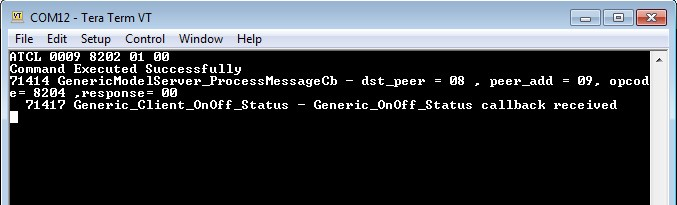
\includegraphics[width=0.99\linewidth]{an5292_atcl_command.png}
	\caption{Wykorzystanie interfejsu szeregowego do wysyłania poleceń. Źródło:~\cite{st_an5292_2021}}
	\label{an5292_atcl_command}
\end{figure}

W analogiczny sposób steruje się poleceniami niezbędnymi do eksperymentu, jak to ukazano na listingu~\ref{lst:at-command}.
\begin{lstlisting}[
    caption={Przykładowe polecenie Mesh Serial Gateway},
    label={lst:at-command}]
ATAP SET-nn iiiiTTTTTTTT src dst

przyklad:
ATAP SET-05 0a6400009c40 03 05
\end{lstlisting}

\begin{description}
\item [ATAP] - polecenie testowe
\item [SET-nn] - polecenie typu SET dla funkcji numeru nn, np. SET-05
\item [iiii] - interwał, częstość zapytań wyrażony w tickach; Wartość 16-bitowa
\item [TTTTTTTT] - czas po którym należy przerwać badanie wyrażone w tickach; Wartość 32-bitowa
\item [src] - adres źródłowego węzła (najczęściej węzła bliższego)
\item [dst] - adres węzła docelowego (najczęściej węzła dalszego)
\end{description}


%%%%%%%%%%%%%%%%%%%%%%%%%%%%%%%%%%%%%%%%%%%%%%%%%%%%%%%%%%%%%%%%%%%%%%%%%%%%%%%%
%% SUBSECTION: Oprogramowanie PC
%%%%%%%%%%%%%%%%%%%%%%%%%%%%%%%%%%%%%%%%%%%%%%%%%%%%%%%%%%%%%%%%%%%%%%%%%%%%%%%%
\subsection{Oprogramowanie PC} \label{prep:pc-software}

Głównym zadaniem oprogramowania PC jest udostępnienie prostego interfejsu
użytkownika umożliwiającego swobodne przeprowadzenie badań, w szczególności PER. 
Stworzenie takie programu umożliwia nie tylko szybsze wykonanie doświadczeń, co
również redukuje błędy możliwe do popełnienia podczas ręcznego wprowadzania 
komend \gls{AT}.

Aplikacja realizuje trzy główne cele: 
\begin{itemize}
\item Ustanawia połączenie z mikrokontrolerem przy użyciu portu szeregowego
\item Umożliwia kalibrację podstawy mikrokontrolera czasu względem ticknięć 
\item Umożliwia wykonanie poleceń uruchamiających cykl badań PER i odbiór wartości
zliczeń z~węzła dystalnego
\end{itemize}

Oprogramowanie wykonano z wykorzystaniem frameworka Qt\footnote{\url{https://www.qt.io/}}.
Umożliwia on tworzenie kompletnych, wieloplatformowych aplikacji graficznych. Qt nie
ogranicza się jedynie do zapewnienia bibliotek graficznych. Framework zapewnia
dostęp z poziomu \gls{API} do urządzeń i~peryferiów takich jak drukarki,
gamepady, gniazda TCP/IP, stosu Bluetooth (w tym BLE) jak i również,
co jest istotne z punktu widzenia niniejszej pracy, portu szeregowego.

Qt zapewnia kilka możliwości tworzenia GUI wykorzystując tylko kod w języku \textit{C++}
lub rozdzielając część widzialną od części biznesowej z pomocą generatora interfejsu
Qt Designer produkując odpowiedni plik \gls{XML} bądź \textit{QML}. QML jest językiem
deklaratywnym opisujący pożądany efekt graficzny. Do silnika tego narzędzia należy
interpretacja i~wygenerowanie właściwego efektu. Język ten rozszerza możliwości
klasycznego wydania frameworka umożliwiając tworzenie dynamicznych, nowoczesnych 
interfejsów użytkownika działających niezależnie od platformy docelowej.

\subsubsection{Port szeregowy}
Aplikację oparto o połączenie części biznesowej tworzonej w~C++ oraz interfejsie
użytkownika stworzonego w QML. Pierwszym, niezbędnym elementem jest zapewnienie
stabilnej komunikacji z użyciem portu szeregowego\footnote{\url{https://doc.qt.io/qt-5/qserialport.html}}.
Aplikacja wpierw wyszukuje listę portów w danym systemie operacyjnym i prezentuje ją
w przystępny dla użytkownika sposób -- Rysunek~\ref{app_device_selector}.

\begin{figure}[!ht]
	\centering 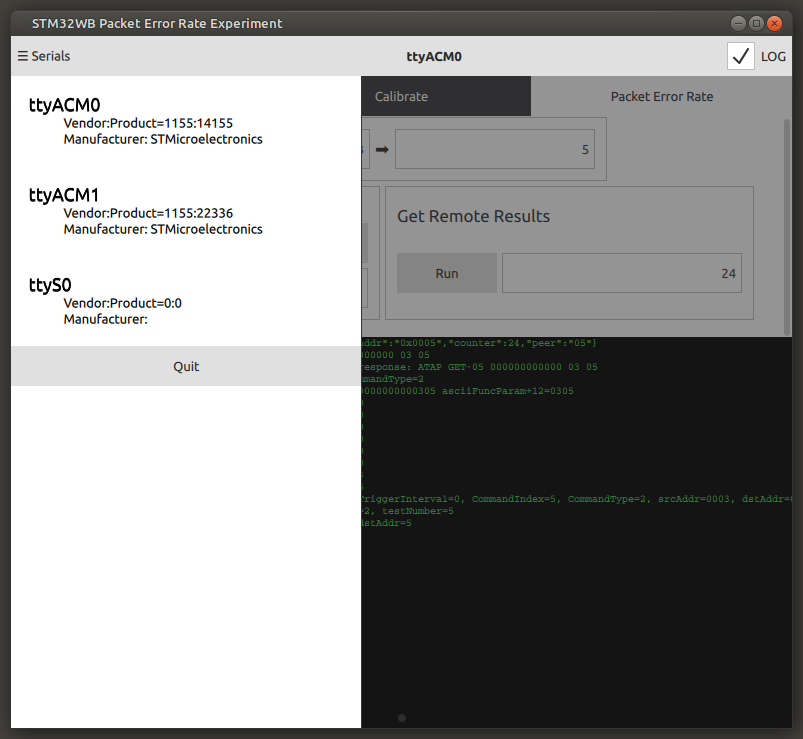
\includegraphics[width=0.618\linewidth]{app_device_selector.png}
	\caption{Selektor portów szeregowych w aplikacji służącej eksperymentowi PER.}
	\label{app_device_selector}
\end{figure}


\subsubsection{Kalibracja}
Kolejnym elementem, wymaganym przez chęć przeprowadzenia badania, jest zapewnienie
właściwej podstawy czasu. Wykorzystywany timer (jak został opisany w punkcie \ref{sec:timer})
wymaga sprecyzowania wartości podanej w tick'ach. Zauważając potencjalny problem
z matematycznym wyznaczeniem odpowiedniego mapowania z milisekund do ticków
zdecydowano się na stworzenie empirycznego sposobu na wyznaczenie tej wartości.

Kalibracja urządzenia polega na odnalezieniu wartości ticków przypadającą na pożądany okres
wyrażony w milisekundach. Usługa obsługująca taką operację przedstawiona została
na listing'u~\ref{lst:calibration_rtc}. Zadaniem aplikacji PC jest jej wielokrotne
wykorzystanie celem wyznaczenia ostatecznej wartości.

\begin{figure}[!ht]
	\centering 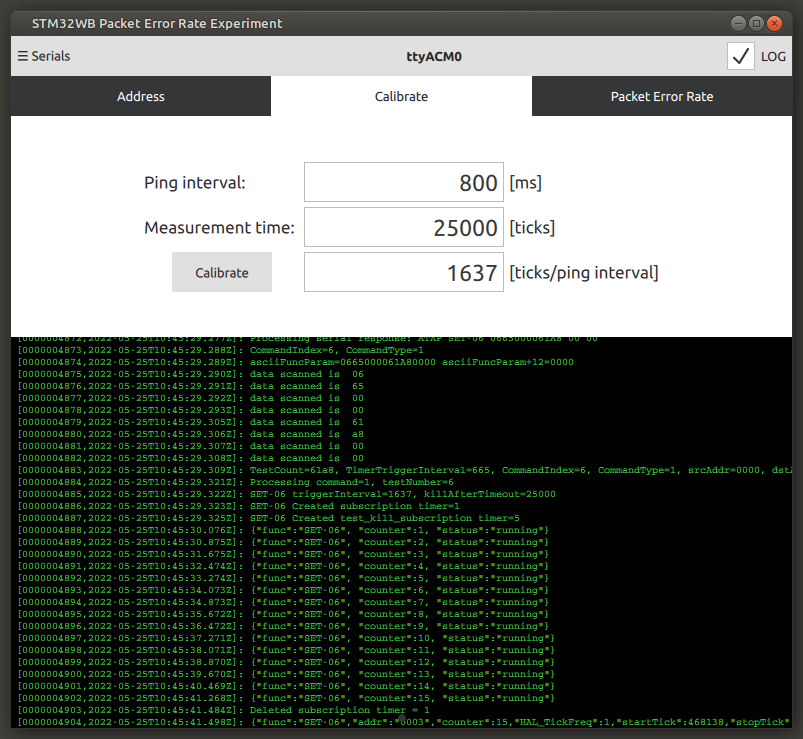
\includegraphics[width=0.618\linewidth]{app_calibration.png}
	\caption{Selektor portów szeregowych w aplikacji służącej eksperymentowi PER.}
	\label{app_calibration}
\end{figure}

Algorytm działania jest następujący. Dla oczekiwanej wartości wyrażonej w milisekundach,
wykonuje się pierwsze polecenie kalibracyjne zakładając fałszywie, iż milisekundy
równe są ilości ticków. Aplikacja, nasłuchuje przychodzące komunikaty w~formacie JSON
poszukując słowa kluczowego \enquote{\textit{status}}. Do każdego zliczonego komunikatu,
aplikacja przechowuje dodatkowo znacznik czasu. Takie wiadomości akumulowane są 
w pamięci do momentu otrzymania innego słowa kluczowego: \enquote{\textit{not\_running}}. W tym momencie,
aplikacja wylicza różnicę między przyległymi znacznikami czasowymi (efektywnie je różniczkując
w~liniach 4-9 listingu~\ref{lst:calibration-cpp}). Następnie, wyliczana jest
średnia różnica pomiędzy poszczególnymi okresami, w których otrzymano odpowiedź 
z~mikrokontrolera -- linia~15.

\begin{lstlisting}[language=C,
    caption={Algorytm wyznaczania kolejnej wartości dla funkcjonalności kalibracji},
    label={lst:calibration-cpp}]
// plik calibratecommand.cpp
std::pair<uint16_t, double> CalibrateCommand::computeNewInterval() {
	QVector<qint64> timestampDiffs;
	std::transform(std::cbegin(timestamps), std::cend(timestamps),
		std::back_inserter(timestampDiffs),
		[] (const QDateTime &timestamp) -> long { return timestamp.toMSecsSinceEpoch(); });

	std::adjacent_difference(std::begin(timestampDiffs), std::end(timestampDiffs), std::begin(timestampDiffs));
	timestampDiffs.removeFirst();

	qint64 sum = 0;
	for (qint64 elem : qAsConst(timestampDiffs)) {
		sum += elem;
	}
	double meanTimestampDiff = sum / static_cast<double>(timestampDiffs.size());
	double accuracy = abs((meanTimestampDiff - expectedIntervalMs) / static_cast<double>(expectedIntervalMs));
	double interval = currentIntervalTicks + currentIntervalTicks * accuracy; // this isn't stable if we overshoot the correct value...

	return std::make_pair(interval, abs(accuracy));
}
\end{lstlisting}


Kolejnym krokiem jest wyliczenie procentowej różnicy pomiędzy obecnie wyliczoną wartością
a oczekiwaną wartością wyrażoną w milisekundach -- linia 16. Ostatecznie, wylicza się
nową, estymowaną wartość kolejnej iteracji zgodnie z~zależnością liniową podaną w~linii~17.

Kalibracja zatrzyma się automatycznie, gdy osiągnięta zostanie zbieżność na poziomie poniżej
jednego procenta różnicy. Algorytm jest wrażliwy na \enquote{\textit{przestrzelenie}} kalibrowanej
wartości. Jego jakość jest jednak na tyle wystarczająca, iż ostatecznie umożliwił wyznaczenie
wartości, które są zbieżne z obliczeniami teoretycznymi, co pokazuje tabela~\ref{tab:calibration_vs_computation}.
Możliwym usprawnieniem byłoby zastosowanie metody wyznaczania parametrów
kalibracyjnych w oparciu o analogię do metody bisekcji.

\begin{table}[!ht]
\centering
	\begin{tabular}{r|r|r|r}
	Ping [ms]         & Skalibrowane [tick] & Obliczone [tick]  & Różnica [\%] \\\hline
	100               & 204                 & 204.59            & 0.29         \\\hline
	500               & 1022                & 1022.95           & 0.09         \\\hline
	800               & 1637                & 1636.72           & 0.02         \\\hline
	1300              & 2661                & 2659.68           & 0.05         \\\hline
	2100              & 4299                & 4296.40           & 0.06         \\\hline
	\end{tabular}
\caption{\label{tab:calibration_vs_computation}Zebrane empirycznie współczynniki kalibracyjne w~porównaniu z~wartościami obliczonymi}
\end{table}

\subsubsection{Badanie PER i odczyt wyników}
Głównym zadaniem aplikacji jest oczywiście przeprowadzenie doświadczenia PER. W~tym celu
stworzono wygodny interfejs do m.in. funkcji opisywanej w punkcie~\ref{sec:proximal-node}.
Aplikacja wymaga od użytkownika podania adresu (od lewej): węzła bliższego oraz
węzła dalszego. W~rzędzie poniżej znajdują kontenery z~dwoma funkcjami w~danej zakładce:
właściwy test PER oraz odbiór wartości z~węzła zewnętrznego -- Rysunek~\ref{app_per_measurement}.
 
\begin{figure}[!ht]
	\centering 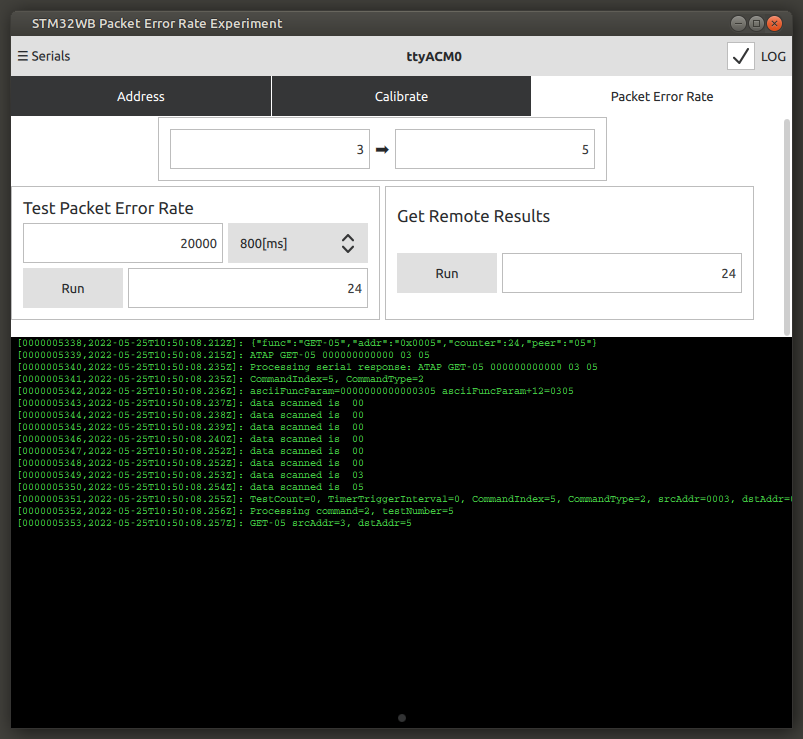
\includegraphics[width=0.618\linewidth]{app_per_measurement.png}
	\caption{Właściwy interfejs użytkownika do przeprowadzenia doświadczenia PER}
	\label{app_per_measurement}
\end{figure}

Eksperymentator, w celu przeprowadzenia doświadczenia, zobowiązany jest wyznaczyć okres, po 
którym zakończy się badanie w~milisekundach. Czas badania powinien być dostatecznie
długi, by błędy inicjalizacji, czy konwersji milisekund do ticków nie miały znacznego wpływu
na otrzymany rezultat. Drugi parametr to interwał odpytywania. Aplikacja przechowuje
wyniki kalibracyjne\footnote{wykorzystując możliwości \href{https://doc.qt.io/qt-5/qsettings.html}{\textit{QSettings}}
dane przechowywane są trwale na dysku. W zależności od systemu albo w rejestrze (Windows),
albo w pliku \texttt{\textasciitilde{}/.config/Warsaw University of Technology/STM32WB Packet Error Rate Experiment.conf} (*nix)},
by je wykorzystać właśnie w tym miejscu. Przyśpiesza to procedurę badawczą, a przede wszystkim
zmniejsza ryzyko błędu. Ostatnim elementem jest przycisk \enquote{Run}, który uruchamia procedurę
badawczą. Ekran aplikacji zostanie zablokowany na czas badania.

Analogicznie należy postąpić w~przypadku odczytywania licznika z węzła dalszego. Użytkownik
zobowiązany jest kliknąć przycisk \enquote{Run} w kontenerze \enquote{\textit{Get Remote Results}}.
Po krótkiej chwili, odpowiadające pole powinno zostać zaktualizowane o~oczekiwaną wartość.


%%!!!!!!!!!!!!!!!!!!!!!!!!!!!!!!!!!!!!!!!!!!!!!!!!!!!!!!!!!!!!!!!!!!!!!!!!!!!!!!
%%%%%%%%%%%%%%%%%%%%%%%%%%%%%%%%%%%%%%%%%%%%%%%%%%%%%%%%%%%%%%%%%%%%%%%%%%%%%%%%
%% SECTION: Zużycie energii
%%%%%%%%%%%%%%%%%%%%%%%%%%%%%%%%%%%%%%%%%%%%%%%%%%%%%%%%%%%%%%%%%%%%%%%%%%%%%%%%
%%!!!!!!!!!!!!!!!!!!!!!!!!!!!!!!!!!!!!!!!!!!!!!!!!!!!!!!!!!!!!!!!!!!!!!!!!!!!!!!
\section{Badanie zużycia energii}\label{experiment:energy-consumption}
Celem niniejszego podrozdziału jest omówienie empirycznej weryfikacji
zużycia energii przez wybrany zestaw uruchomieniowy \gls{BLE}.

Zaprezentowanie zostanie metodologia pomiaru oraz sposób połączenia
układu pomiarowego. Omówione zostaną parametry próbkowania i długość trwania
pojedynczej sesji badawczej. Ostatecznie, przedstawia się wzór i~sposób
przeprowadzonych obliczeń, które docelowo zapewniają oczekiwane wyniki.

Ostatnim, aczkolwiek najistotniejszym elementem poruszanym przez podrozdział,
jest prezentacja wyników. Pogrupowane są one na dwie kategorie: BLE Heart Rate
i BLE Mesh. Każda z~nich przedstawia zebrane empirycznie dane, wskazując
na właściwe tryby działania i~całkowite zużycie energii.

%%%%%%%%%%%%%%%%%%%%%%%%%%%%%%%%%%%%%%%%%%%%%%%%%%%%%%%%%%%%%%%%%%%%%%%%%%%%%%%%
%% SUBSECTION: Metodologia badania
%%%%%%%%%%%%%%%%%%%%%%%%%%%%%%%%%%%%%%%%%%%%%%%%%%%%%%%%%%%%%%%%%%%%%%%%%%%%%%%%
\subsection{Metodologia badania}

Podstawą badania zużycia energii jest pomiar wartości pobieranego prądu przez zestaw uruchomieniowy
P-NUCLEO-WB55 w czasie. Posiadając dane wymienione dane, na podstawie oczywistych
zależności fizycznych wyznacza się parametry jak całkowita wykorzystana energia
podczas badania, przedstawiona w przystępnej postaci parametru mocy.

Pomiary wartości chwilowego poboru prądu oparto o moduł opisany w punkcie~\ref{device:plytka_pomiarowa}.
Źródłem energii dla płytki pomiarowej jest komputer klasy PC, a precyzyjniej udostępniany
port USB. Wykorzystując również ten protokół następuje transmisja danych poprzez komunikację szeregową
UART, umożliwiając akwizycję danych.

Połączenie z zestawem uruchomieniowym oparto o konektor CN14 udostępniający piny: PIN1 - masa GND, PIN3 - VCC $3.3V$~\cite{noauthor_um2243_2018}.
Wyprowadzone przewody połączono następnie z P-NUCLEO-WB55 poprzez konektor JP2, wcześniej pozbawiony zawleczki.
Jest to metoda rekomendowana dla pomiaru prądu opisana w dokumentacji zestawu~\cite{stmicroelectronics_um2435_2019}\footnote{
Rozdział 7.12 Current measurement}. Porty kompatybilne z Arduino/ST Morpho mogłyby stanowić równorzędny sposób
włączenia zestawu uruchomieniowego do obwodu płytki pomiarowej. Autorska analiza dokumentacji sugeruje jednak,
iż opcja ta nie jest wspierana. Wymagane byłoby lutowanie dodatkowego połączenia w (punkcie SB27), by móc wykorzystać
zasilanie napięciem $3.3V$.

\begin{figure}[!htb]
	\centering 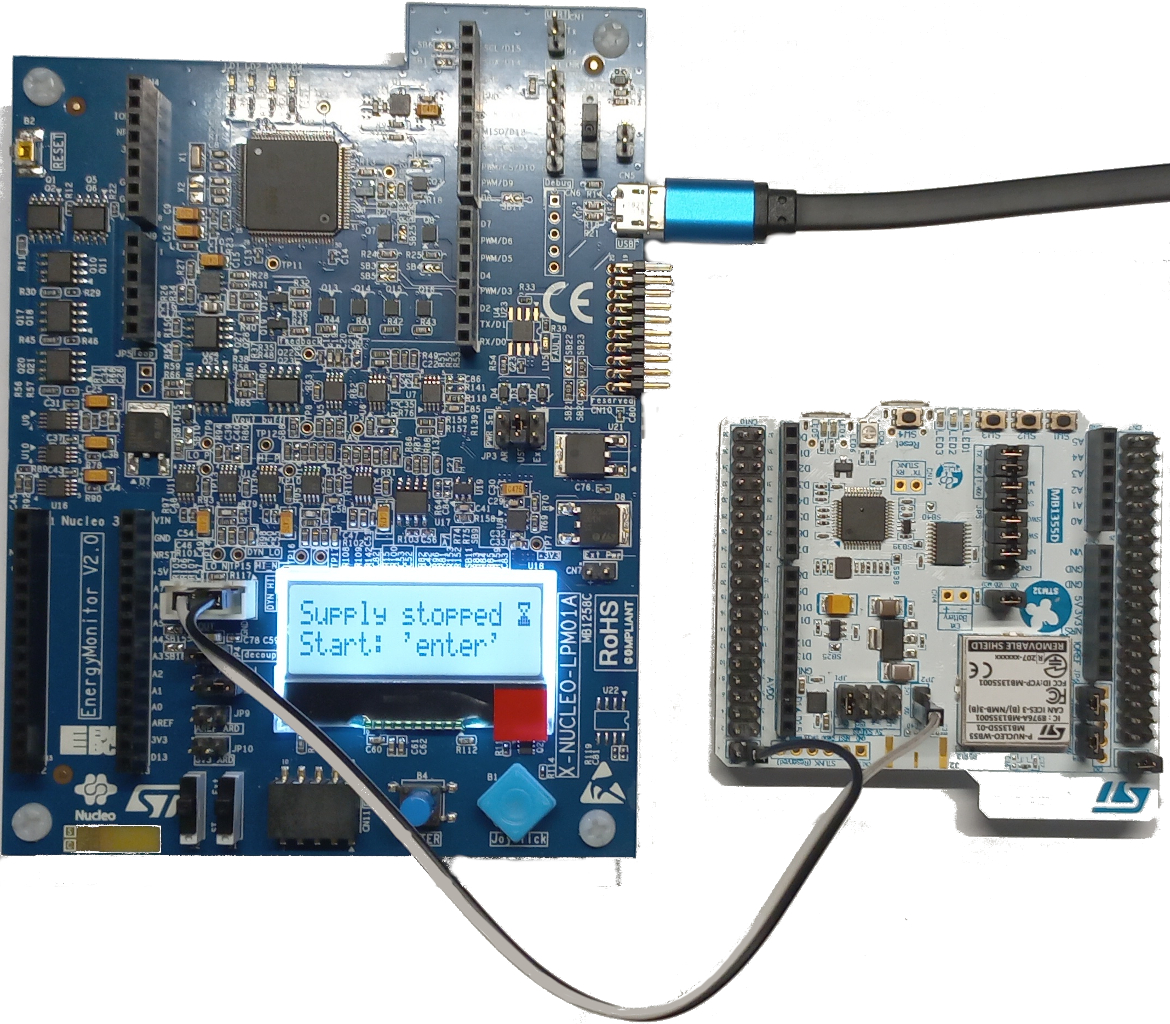
\includegraphics[width=0.618\linewidth]{power_measurement_unit_connected.png}
	\caption{Podłączony zestaw pomiarowy}
	\label{rys:connected_power_measurement_unit}
\end{figure}

Celem akwizycji danych wybrano dostarczane przez producenta oprogramowanie \textit{STM32CubeMonitor-Power}.
Pojedyncza sesja pomiarowa trwająca 100 sekund zapewnia niezbędne dane. Są one następnie
odpowiednio przetwarzane poprzez odcięcie wartości zebranych w ostatnich sekundach. Związane to było
ze sposobem działania mikrokontrolera, który po 60 sekundach przechodzi w stan zwiększonej
oszczędności energii. Stąd, by rozróżnić różne tryby pracy \gls{BLE}, zdecydowano o odcięciu
połowy okresu pomiarowego, zapewniając jednolite wartości względem trybów zużycia energii
w~50 sekundowym oknie.

\begin{figure}[!htb]
	\centering 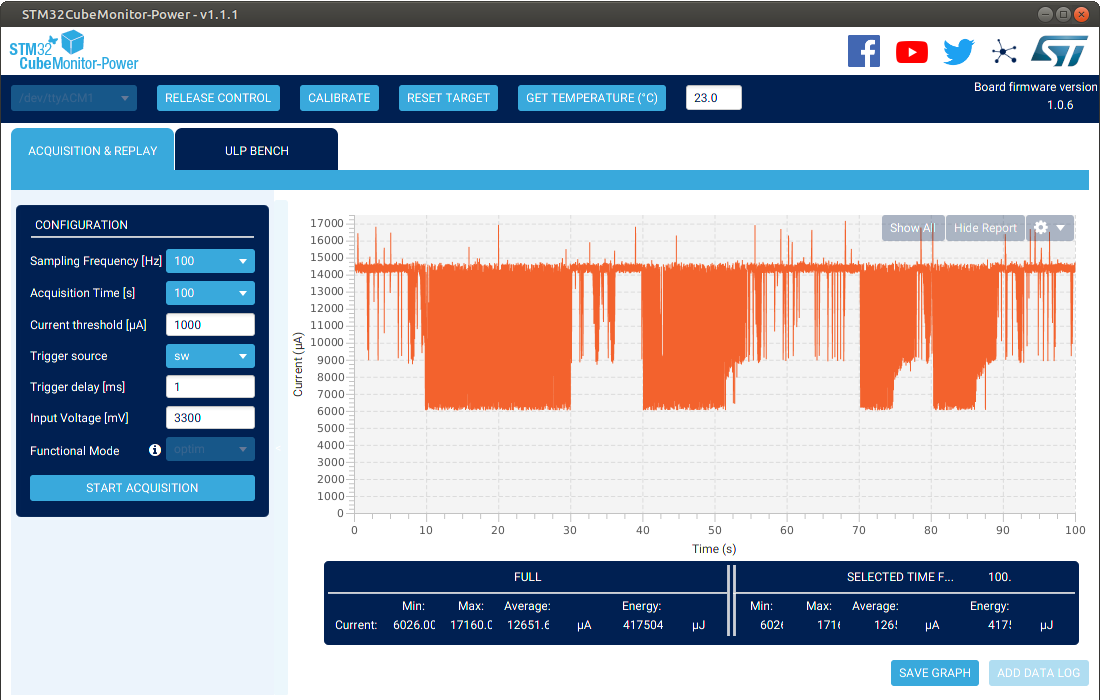
\includegraphics[width=0.99\linewidth]{stm32_power_monitor_sample.png}
	\caption{Przykładowa sesja pomiarowa dla BLE Mesh - sieć w trybie nasłuchującym}
	\label{rys:measurement_session_sample}
\end{figure}

Tak zebrane dane następnie przetworzono uzyskując wartości energii i średniej mocy
użytej przez układ. Wykorzystuje się w celu oczywistą zależność fizyczną zaprezentowaną
wzorem~\ref{energy_equation}\cite{skoro_marta_fizyka_1973}.

\begin{equation} \label{energy_equation}
E_{\text{całkowita}} = U \cdot \int_{t=0[s]}^{t=50[s]} \mathrm{d}i \: \mathrm{d} t
\end{equation}

\begin{equation} \label{power_equation}
P = \frac{E_{\text{całkowita}}}{t}
\end{equation}

gdzie:

\begin{description}
\item $E_{\text{całkowita}} [J]$ - wykorzystana energia podczas 50s sekundowej sesji rejestracji danych
\item $P [W]$ - moczużyta podczas 50s sekundowej sesji rejestracji danych
\item $U [V]$ - napięcie zasilania mikrokontrolera - 3.3V - stała
\item $\mathrm{d}i [A]$ - prąd w danej chwili
\item $\mathrm{d}t [s]$ - podstawa czasowa całkowania, 0.01s/interwał (100Hz) - stała 
\end{description}

Zebrane dane w postaci wartości chwilowych pobieranego przez mikrokontroler prądu względem czasu
przetworzono z użyciem metod numerycznych. W~celu wyliczenia łącznej wykorzystanej energii, a~tym samym
mocy, stosuje się zależność~\ref{energy_equation}. Uwzględniając fakt działania w domenie dyskretnej,
wykorzystano kompozytową metodę całkowania Simpsona~\cite{noauthor_scipyintegratesimpson_nodate}.
Podstawą dla całkowania są wartości zebrane w równoodległych odstępach. Dokonując akwizycji danych
dobrano częstotliwość próbkowania jako $100Hz$. Każda kolejna wartość charakteryzuje się więc
10 milisekundową różnicą w~podstawie czasu. Uwzględniając ten fakt, wyliczenie wartości
wykorzystanej energii jak i~mocy staje się trywialne.

%%%%%%%%%%%%%%%%%%%%%%%%%%%%%%%%%%%%%%%%%%%%%%%%%%%%%%%%%%%%%%%%%%%%%%%%%%%%%%%%
%% SUBSECTION: BT Low Energy - Usługa Heart Rate
%%%%%%%%%%%%%%%%%%%%%%%%%%%%%%%%%%%%%%%%%%%%%%%%%%%%%%%%%%%%%%%%%%%%%%%%%%%%%%%%
\subsection{BT Low Energy - Usługa Heart Rate}

\lipsum[1-3]
\begin{figure}[!htb]
	\centering 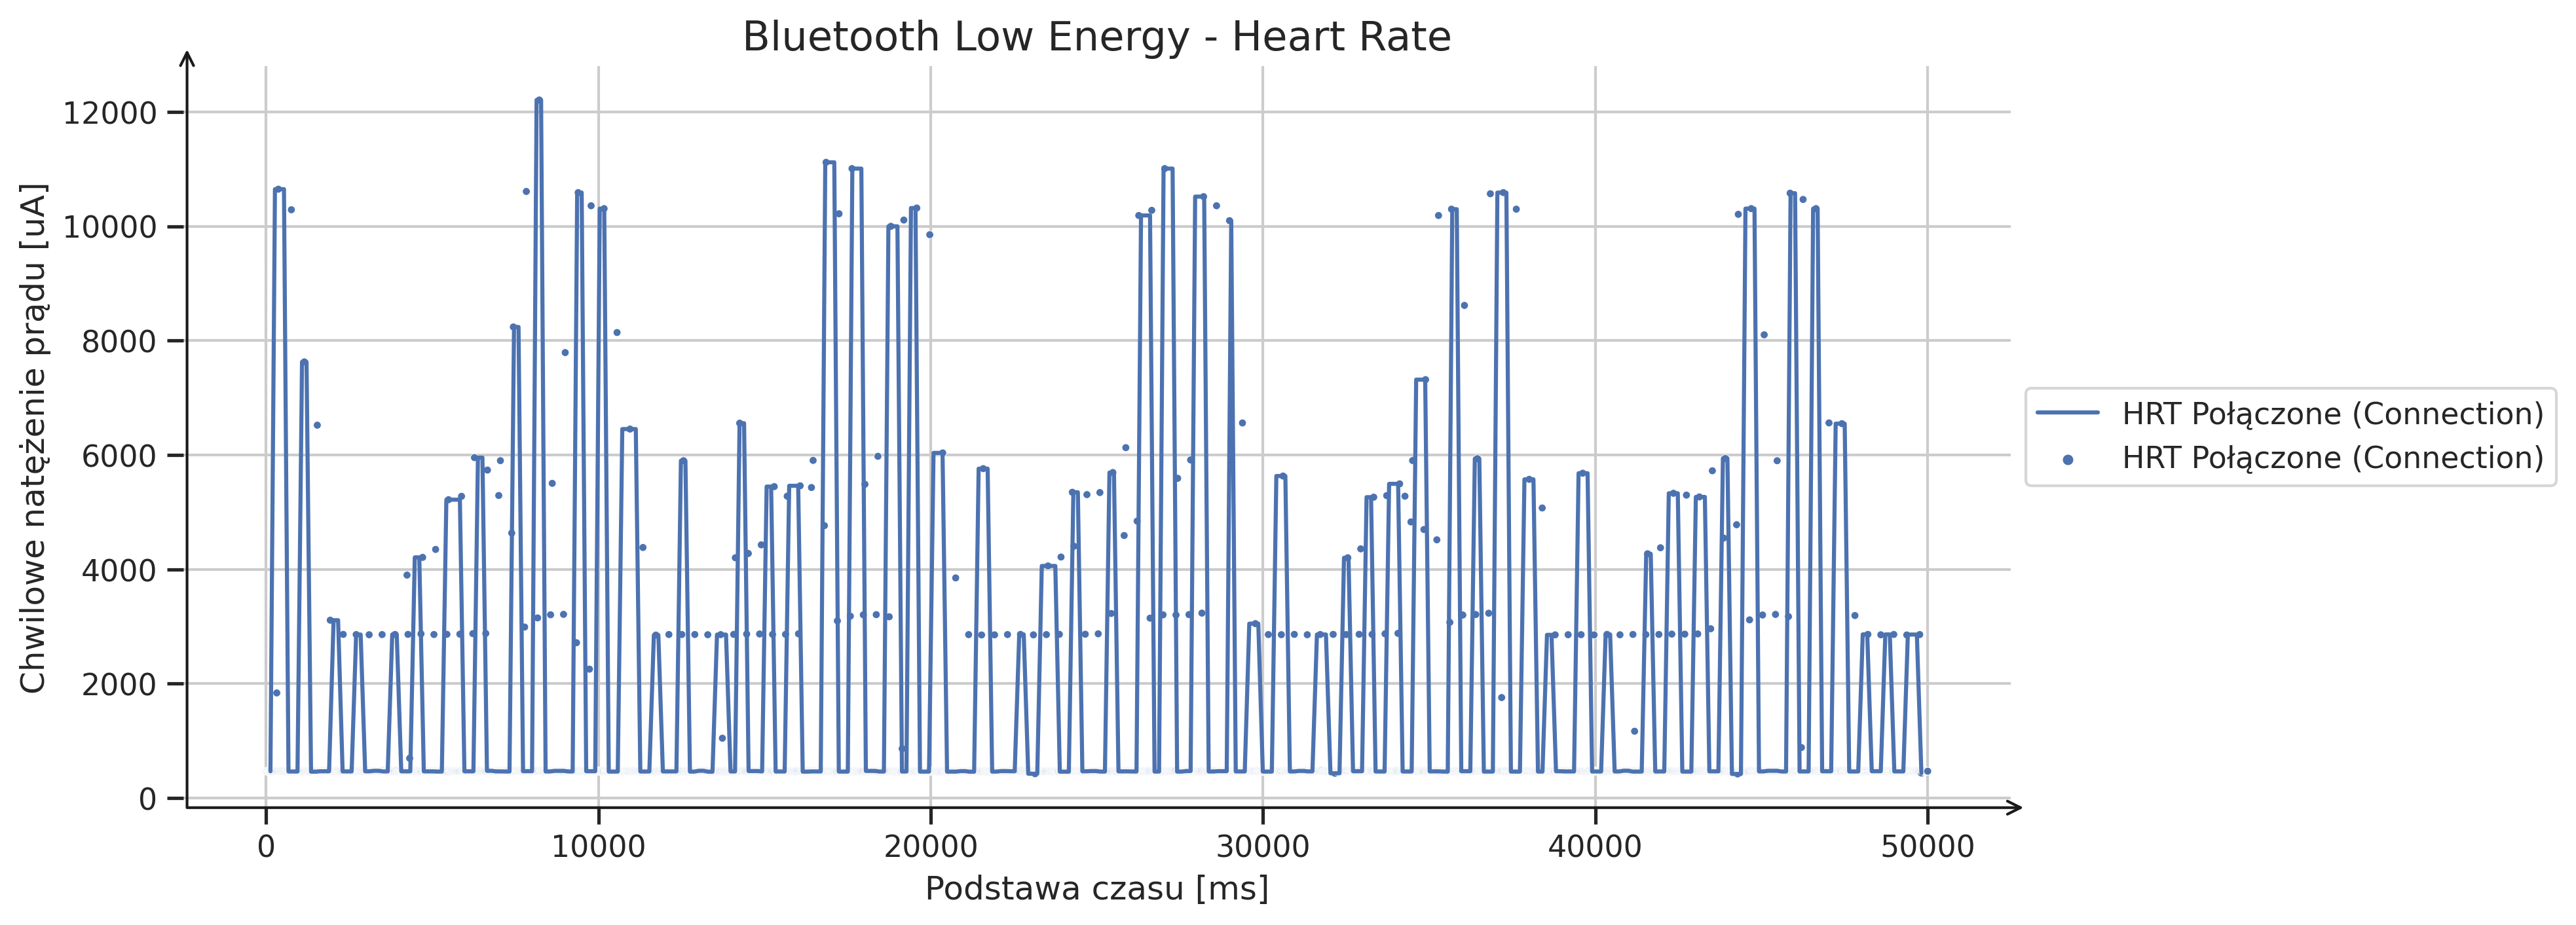
\includegraphics[width=0.99\linewidth]{power_ble_hr_connected_only_amps.png}
	\caption{Charakterystyka czasowa poboru prądu dla BLE i usługi Heart Rate - Usługa Połączona}
	\label{rys:power_ble_hr_connected_only_amps}
\end{figure}

\lipsum[1-3]
\begin{figure}[!htb]
	\centering 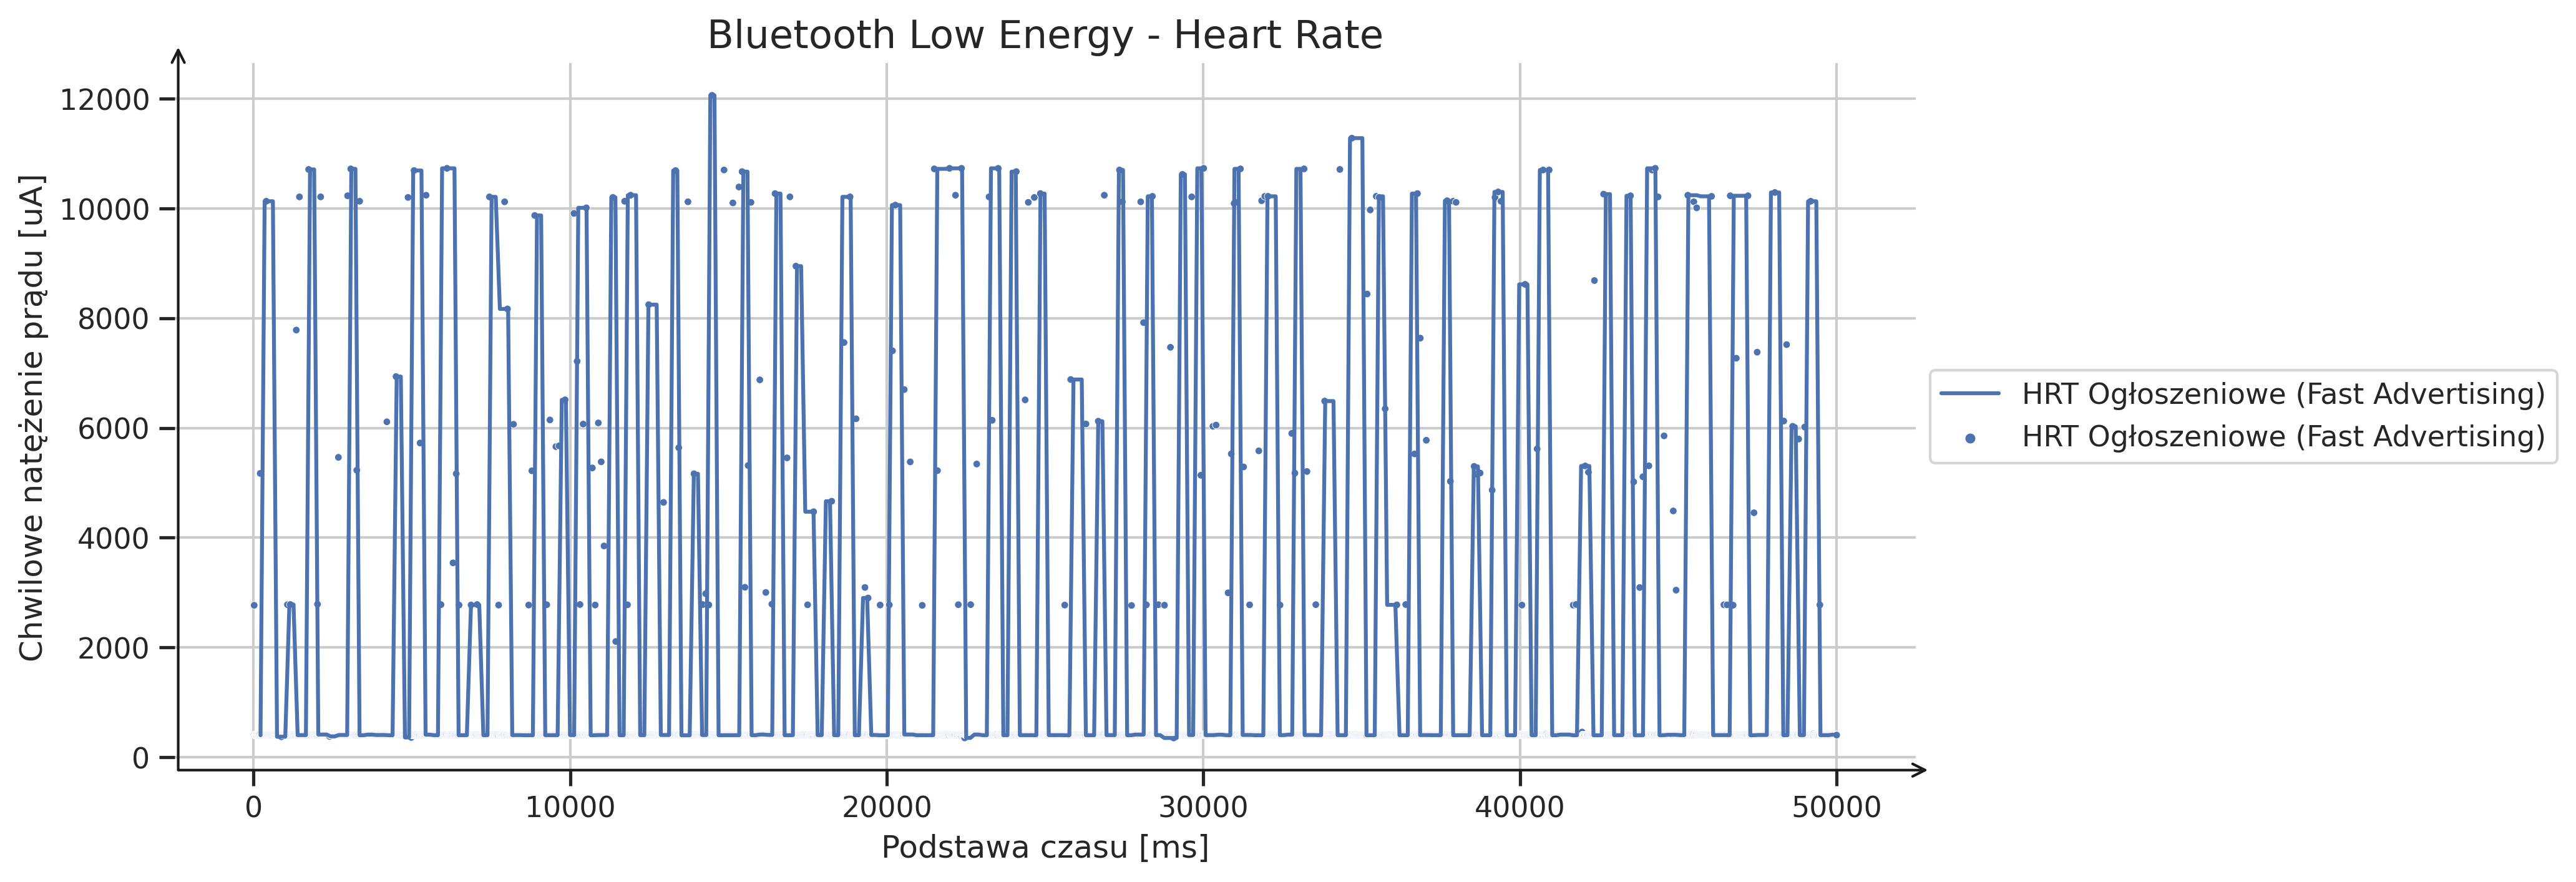
\includegraphics[width=0.99\linewidth]{power_ble_hr_fastadv_only_amps.png}
	\caption{Charakterystyka czasowa poboru prądu dla BLE i usługi Heart Rate - Tryb szybkiego ogłoszenia}
	\label{rys:power_ble_hr_fastadv_only_amps}
\end{figure}

\lipsum[1-3]
\begin{figure}[!htb]
	\centering 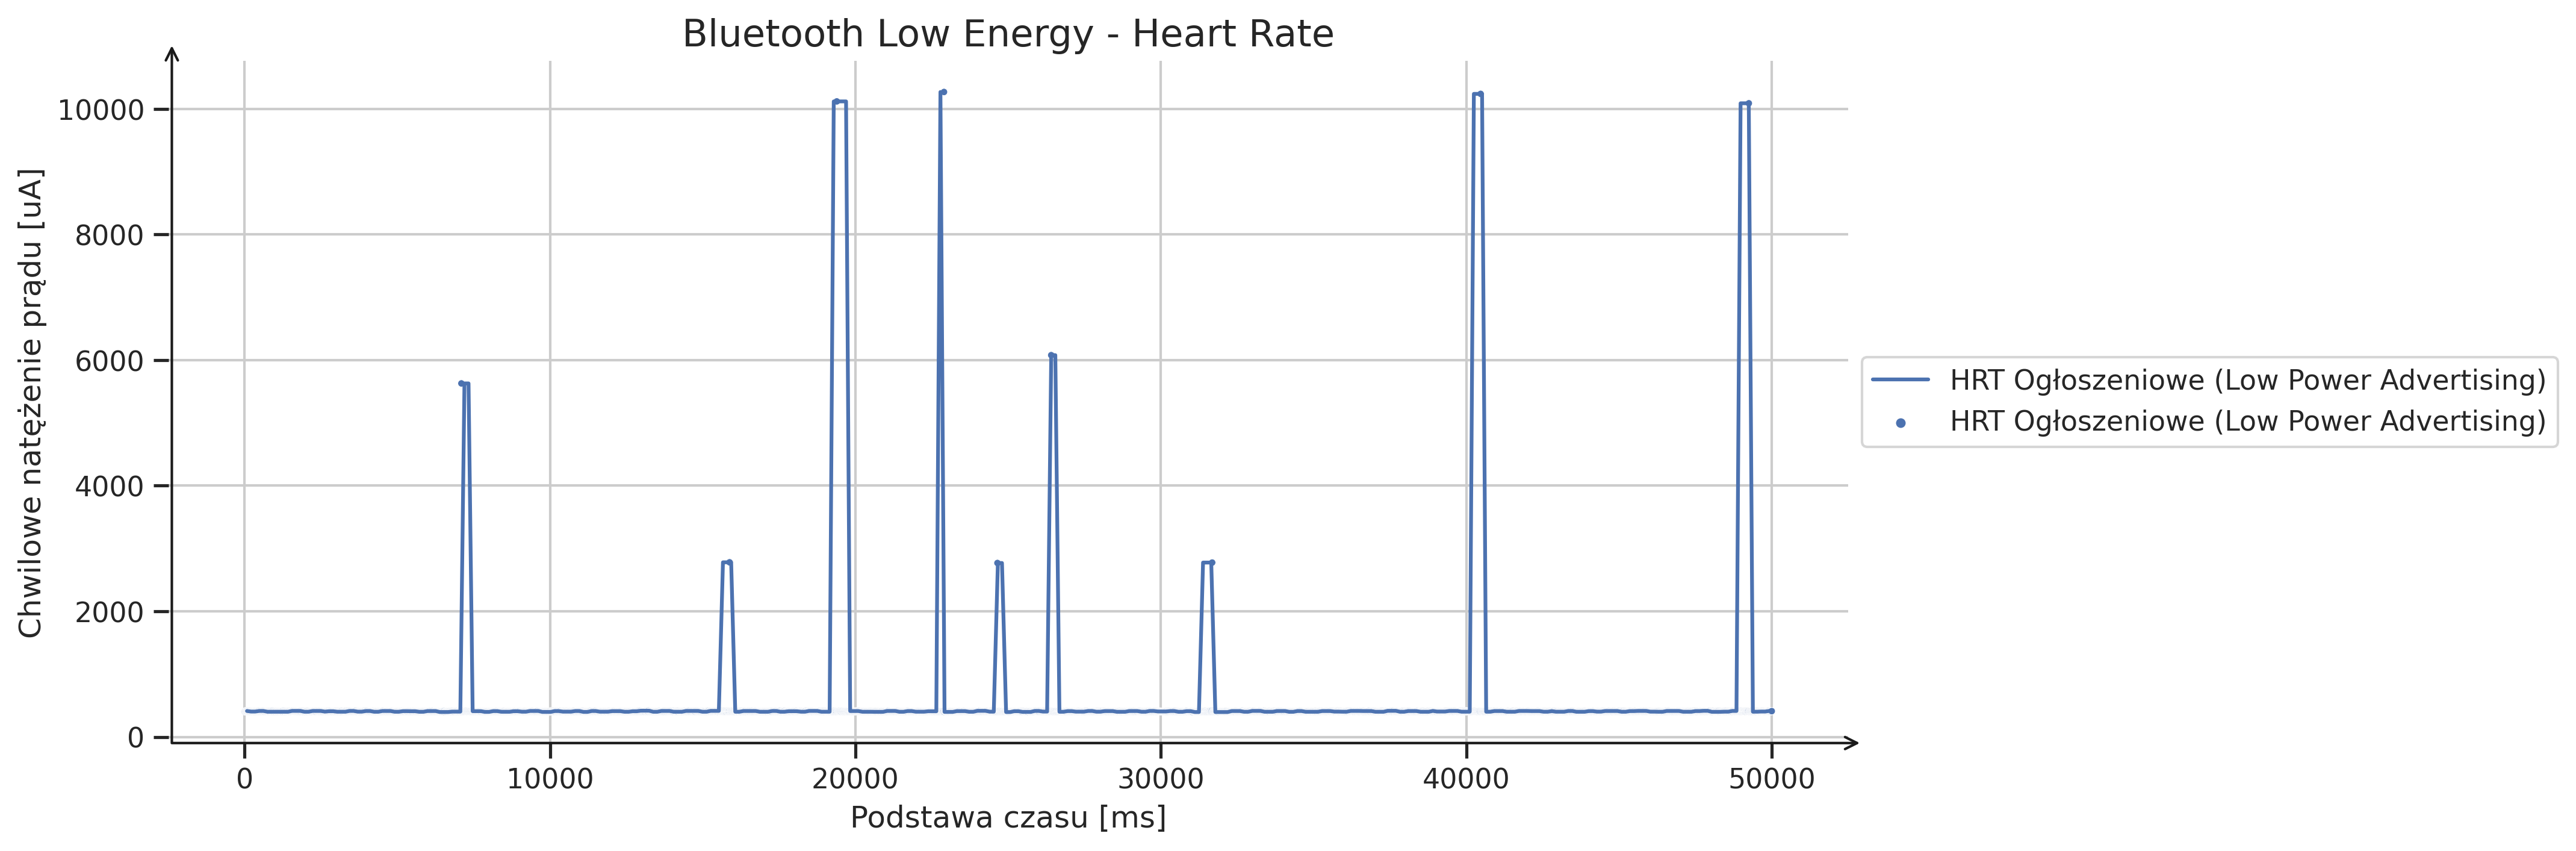
\includegraphics[width=0.99\linewidth]{power_ble_hr_low_power_adv_only_amps.png}
	\caption{Charakterystyka czasowa poboru prądu dla BLE i usługi Heart Rate - Tryb małomocowego ogłoszenia}
	\label{rys:power_ble_hr_low_power_adv_only_amps}
\end{figure}


\lipsum[1-2]
\begin{figure}[!htb]
	\centering 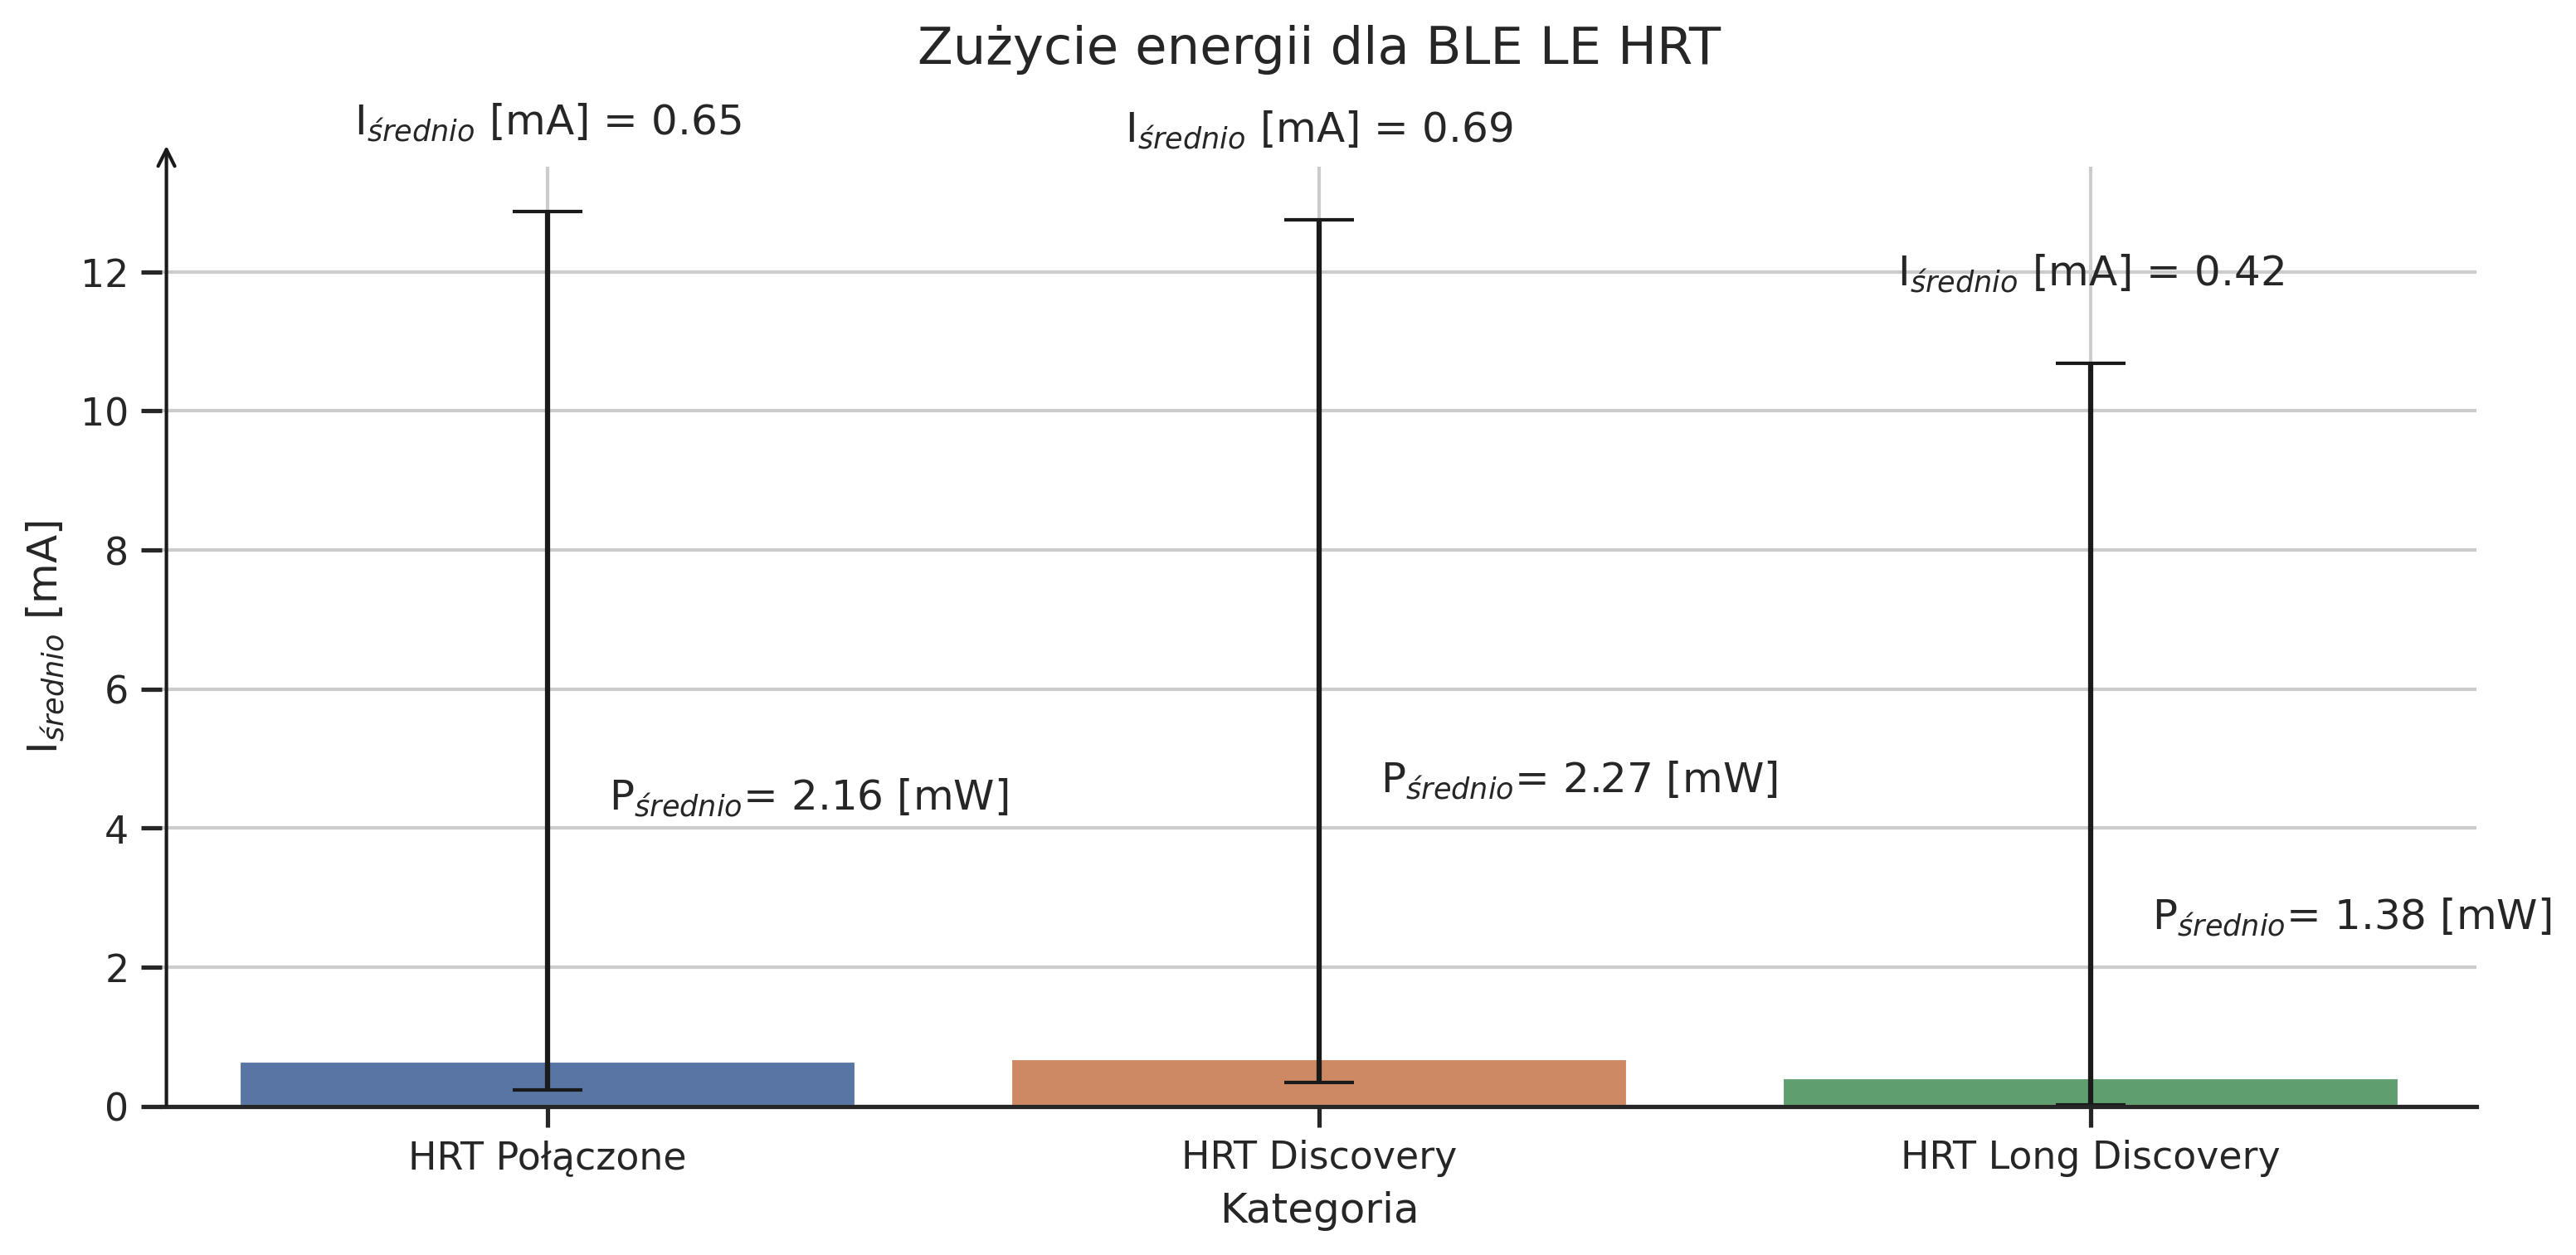
\includegraphics[width=0.99\linewidth]{power_ble_hr_amps_usage_juxtaposition.png}
	\caption{Zestawienie zużycia prądu dla usługi Heart Rate w zależności od trybu działania}
	\label{rys:power_ble_hr_amps_usage_juxtaposition}
\end{figure}
\lipsum[1-3]

%%%%%%%%%%%%%%%%%%%%%%%%%%%%%%%%%%%%%%%%%%%%%%%%%%%%%%%%%%%%%%%%%%%%%%%%%%%%%%%%
%% SUBSECTION: BLE Mesh - Model Generic OnOff
%%%%%%%%%%%%%%%%%%%%%%%%%%%%%%%%%%%%%%%%%%%%%%%%%%%%%%%%%%%%%%%%%%%%%%%%%%%%%%%%
\subsection{BLE Mesh - Model Generic OnOff}

Pomiary dla BLE Mesh uwzględniające dwa tryby działania: sieć w oczekująca na komunikaty oraz podczas działania aktywnego korzystania z Modelu Generic OnOff.

\begin{figure}[!htb]
	\centering 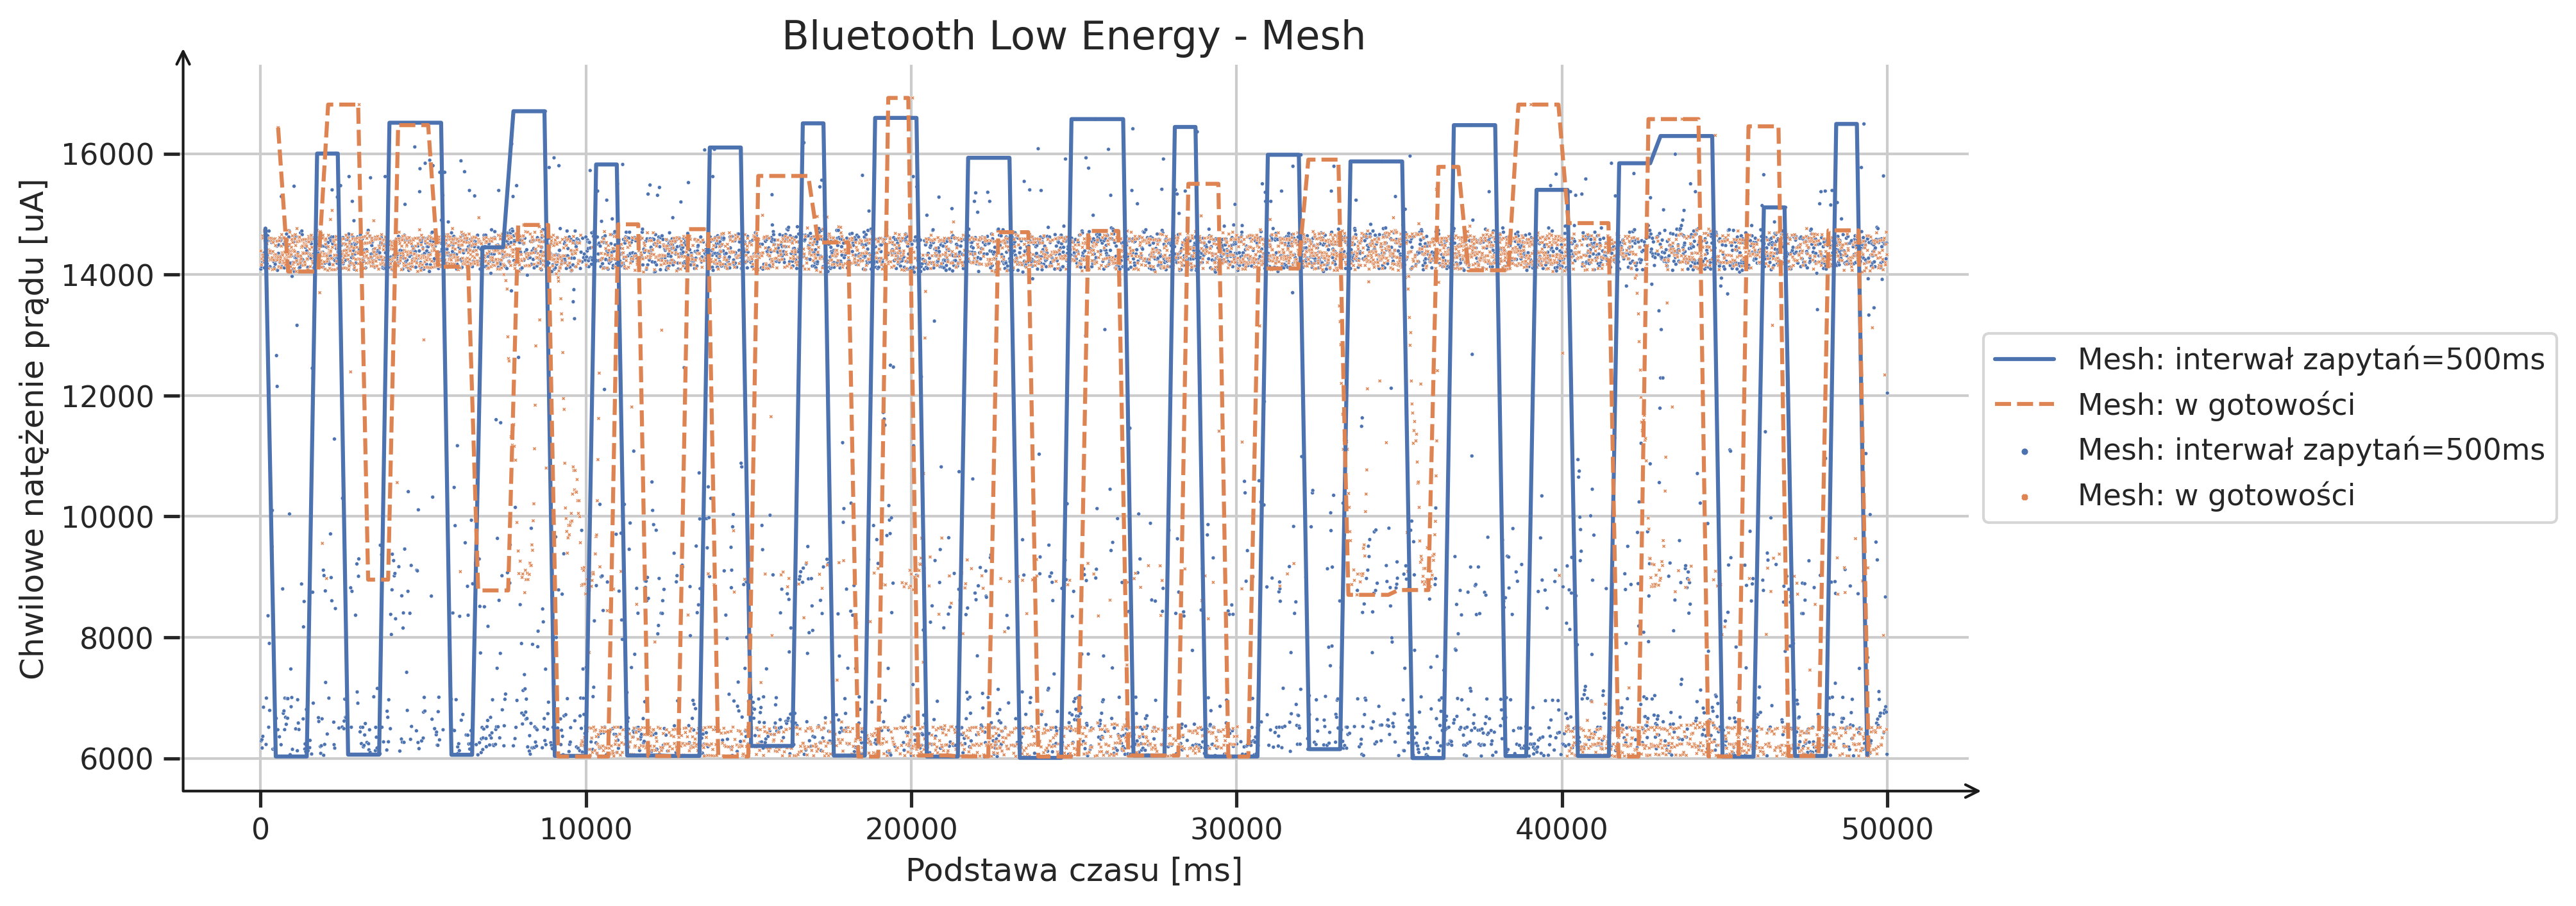
\includegraphics[width=0.99\linewidth]{power_ble_mesh_amps_no_led.png} 
	\caption{Charakterystyka czasowa poboru prądu dla BLE Mesh i modelu Generic OnOff}
	\label{rys:power_ble_mesh_amps}
\end{figure}

\lipsum[1-3]
\begin{figure}[!htb]
	\centering 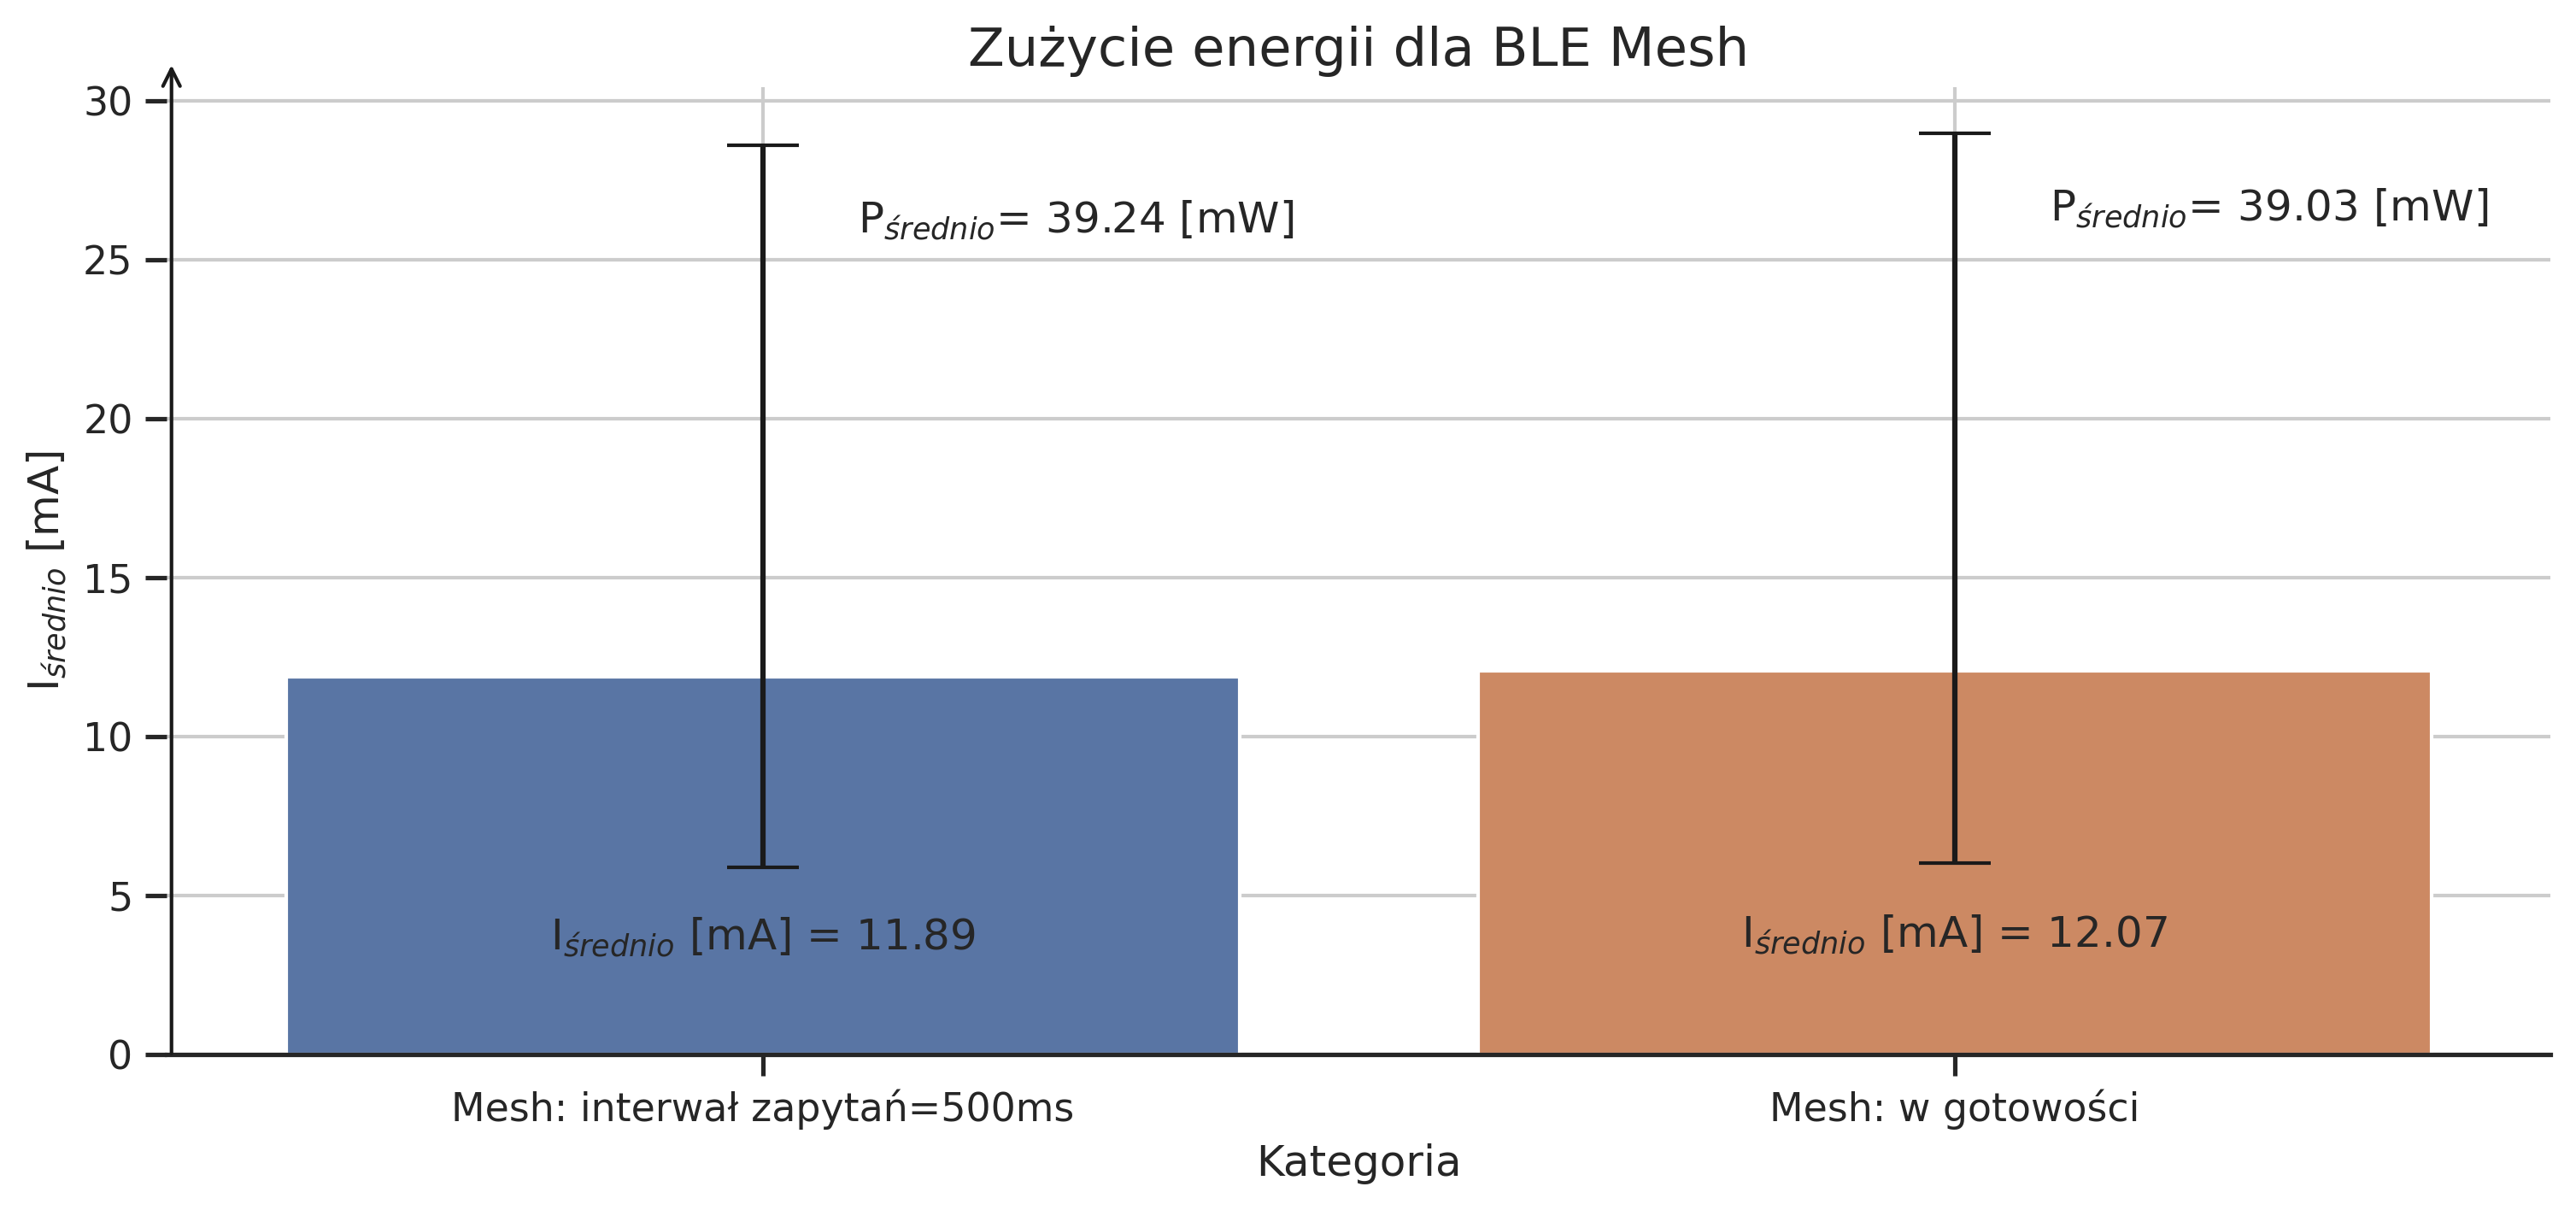
\includegraphics[width=0.99\linewidth]{power_ble_mesh_amps_usage_juxtaposition_no_led.png} 
	\caption{Zestawienie zużycia prądu dla BLE Mesh w zależności od trybu działania}
	\label{rys:power_ble_mesh_amps_usage_juxtaposition}
\end{figure}

\lipsum[1-3]
\begin{figure}[!htb]
	\centering 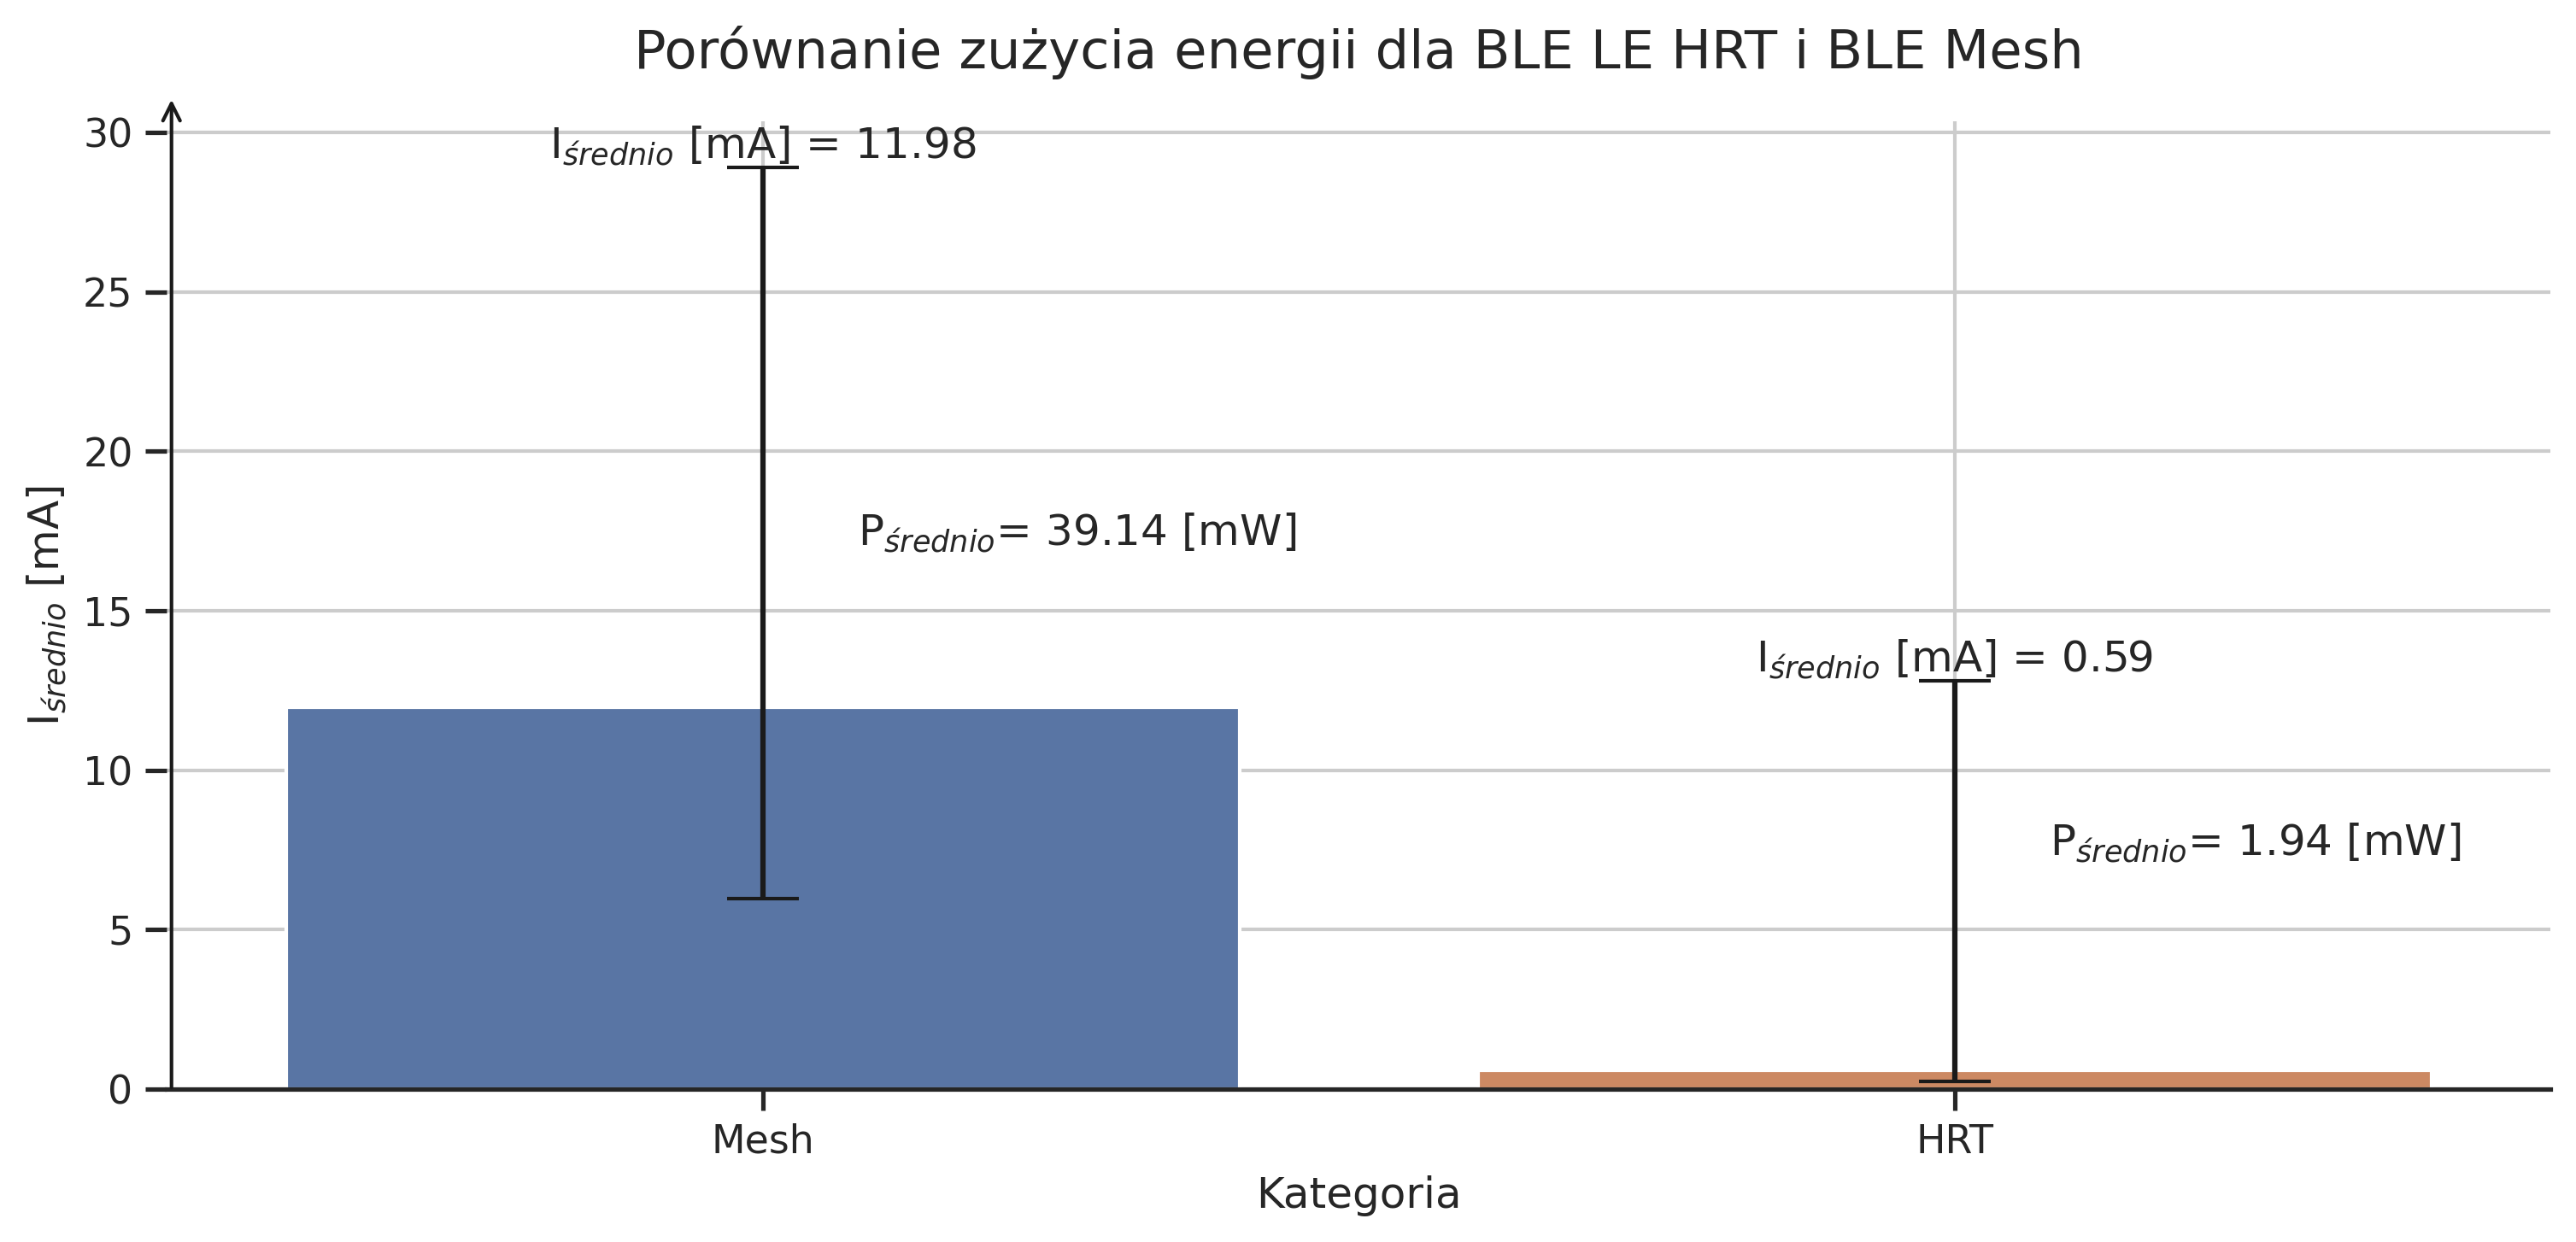
\includegraphics[width=0.99\linewidth]{power_ble_consumption_comparison_no_led.png} 
	\caption{Porównanie średniego zużycia energii pomiędzy BT Low Energy HRT i BLE Mesh}
	\label{rys:power_ble_consumption_comparison}
\end{figure}




%%!!!!!!!!!!!!!!!!!!!!!!!!!!!!!!!!!!!!!!!!!!!!!!!!!!!!!!!!!!!!!!!!!!!!!!!!!!!!!!
%%%%%%%%%%%%%%%%%%%%%%%%%%%%%%%%%%%%%%%%%%%%%%%%%%%%%%%%%%%%%%%%%%%%%%%%%%%%%%%%
%% SECTION: Packet Error Rate
%%%%%%%%%%%%%%%%%%%%%%%%%%%%%%%%%%%%%%%%%%%%%%%%%%%%%%%%%%%%%%%%%%%%%%%%%%%%%%%%
%%!!!!!!!!!!!!!!!!!!!!!!!!!!!!!!!!!!!!!!!!!!!!!!!!!!!!!!!!!!!!!!!!!!!!!!!!!!!!!!
\section{Badanie Packet Error Rate}\label{experiment:per}

Celem niniejszego podrozdziału jest omówienie przeprowadzonego eksperymentu \gls{PER}. Przedstawiona zostanie
metodologia badań oraz zbierane parametry wraz z~ich opisem i uzasadnieniem.

Wychodząc z definicji, badany problem zdefiniowany jest przedstawionym wcześniej równaniem~\ref{per_equation}.
Stanowi ono podstawę dla eksperymentu. Jego zrozumienie pozwoliło zaprojektowanie właściwego doświadczenia
jak i~przygotowanie kompletnego stosu technologicznego niezbędnego do jego przeprowadzenia.

Ostatecznym efektem przeprowadzonego eksperymentu jest przedstawienie zebranych danych w~postaci
wykresów. Prezentują one badane cechy zmienne, zaprezentowane opisane w~sekcji opisu metodologii. 
Końcowym krokiem jest wyciągnięcie wniosków z~zebranych danych.
 
\section{Packet Error Rate}

Celem niniejszego podrozdziału jest omówienie przeprowadzonego eksperymentu \gls{PER}. Omówiona zostanie
metodologia badań. Zdefiniowany zostanie termin \textit{pakietu}, który stanowi podstawę dla
doświadczenia.

Wychodząc z definicji, prezentuje się właściwy wzór matematyczny, definiujący badany problem. Równanie
stanowi podstawę dla eksperymentu. Jego zrozumienie pozwoliło zaprojektowanie właściwego doświadczenia
jak i~przygotowanie kompletnego stosu technologicznego niezbędnego do jego przeprowadzenia.

Ostatecznym efektem przeprowadzonego eksperymentu jest przedstawienie zebranych danych pod postacią
wykresów. Prezentują one badane cechy zmienne zaprezentowane w sekcji opisu metodologii. Końcowym
krokiem jest wyciągnięcie wniosków z zebranych danych.
 
%%%%%%%%%%%%%%%%%%%%%%%%%%%%%%%%%%%%%%%%%%%%%%%%%%%%%%%%%%%%%%%%%%%%%%%%%%%%%%%%
%% SUBSECTION: Zależność PER względem odległości między węzłami
%%%%%%%%%%%%%%%%%%%%%%%%%%%%%%%%%%%%%%%%%%%%%%%%%%%%%%%%%%%%%%%%%%%%%%%%%%%%%%%%
\subsection{Metodologia badania}
% poniższe sekcje przerzucić do części teoretycznej
\subsubsection{Definicja pakietu}
Przed przystąpieniem do badań należy precyzyjnie zdefiniować wykorzystywaną terminologię.

Pakietem nazywamy pojedynczą porcję danych przetwarzaną na poziomie warstwy sieciowej modelu ISO OSI \cite{sa_tcpip_nodate}.
Warstwa ta umożliwia routing, adresowanie logiczne oraz przetwarzanie i~dostarczanie pakietów.

\begin{figure}[!ht]
	\centering 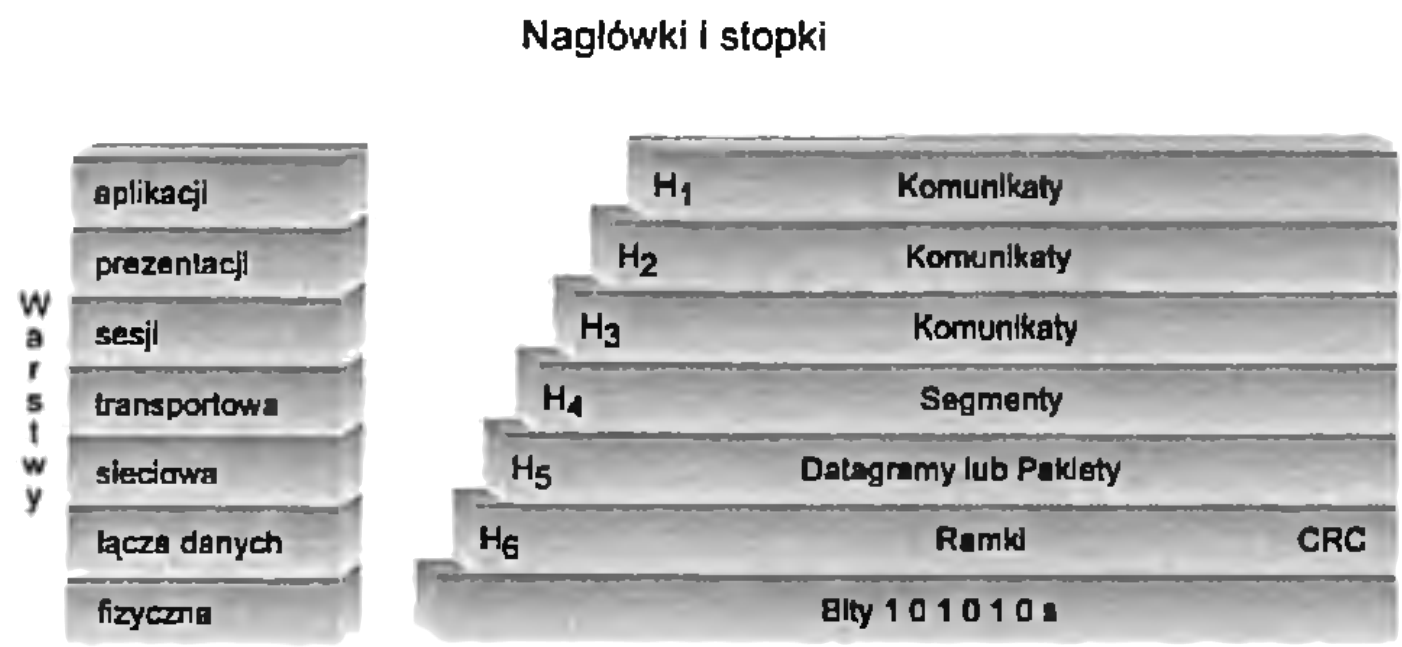
\includegraphics[width=0.618\linewidth]{tcp_ip_szkola_programowania_naglowki_stopki.png} 
	\caption{Model ISO OSI wraz i odpowiadające mu nazwy porcji danych. Źródło: \cite{sa_tcpip_nodate}}
	\label{rys:iso_osi_model_nazwy_grup_danych}
\end{figure}

\gls{BLE} wprowadza własną nomenklaturę dla poszczególnych warstw sieciowych. Jest to o tyle istotne, iż standard ten
nie zapewnia odpowiadających modelowi ISO OSI warstw jeden-do-jednego. Część z tych warstw jest agregowanych w~zespół 
protokołów wyższych warstw - Rysunek~\ref{rys:agregacja_protokolow_ble}. 

Bazując na definicji modelu OSI oraz stosie BLE, pakietem można nazwać wiadomości będące możliwie blisko
warstwy \textit{\gls{LL}}. Podobną definicję prezentuje dokumentacja ST:
\enquote{Pakiet to pojedyncza oznaczona wiadomość wysłana przez jedno i~odebrana przez 
co najmniej jedno urządzenie.}\footnote{Tłumaczenie własne}~\cite{stmicroelectronics_pm0271_2021}

\begin{figure}[!ht]
	\centering 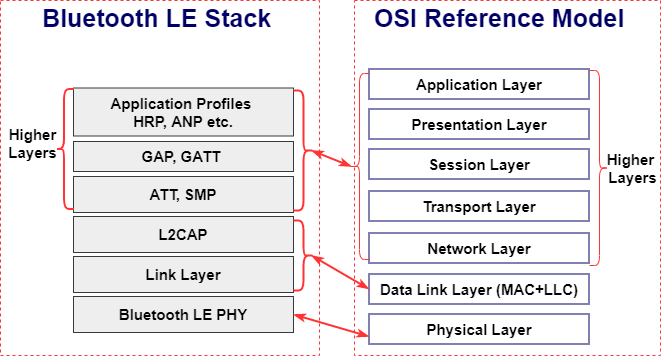
\includegraphics[width=0.618\linewidth]{mathworks_iso_osi_ble_stack.png} 
	\caption{Zestawienie stosu BLE i modelu ISO OSI. Źródło: \cite{noauthor_bluetooth_nodate}}
	\label{rys:agregacja_protokolow_ble}
\end{figure}

BLE Mesh dodatkowo wprowadza własne dodatkowe warstwy komunikacji, biorąc za podstawę stos BLE~\cite{mesh_working_group_mesh_2019}.
Każda z wymienionych warstw jest hermetyzowana za pośrednictwem dostarczanego przez producenta \gls{API}.
Uwzględniając zamknięcie middleware'u i dwu-procesorową architekturę mikrokontrolera STM32WB55, oznacza 
to brak możliwości bezpośredniego nasłuchiwania pakietów w~warstwie \gls{LL}.

Uwzględniając powyższe czynniki, \textit{pakietem} dla BLE Mesh nazywana będzie wiadomość najbliższa warstwie \gls{LL}.
W przypadku stworzonego oprogramowania, oznacza to odbiór komunikatu odebranego jako zdarzenie zarejestrowane przez
koprocesor Cortex-M0, będący integralną częścią mikrokontrolera STM32WB55 odpowiadający za obsługę radia.

\subsubsection{Definicja Packet Error Rate}
Posiadając definicję pakietu, \gls{PER} możliwe staje się zdefiniowanie wzoru, a zarazem znaczenia
głównego celu badań.

PER jest miarą ilości błędnych pakietów w proporcji do wszystkich wysłanych pakietów, zgodnie ze wzorem:

\begin{equation}
\label{per_equation}
PER = \frac{s - r}{s} \cdot 100\%
\end{equation}

gdzie:

\begin{description}
\item[s] is ilość wysłanych pakietów
\item[r] is ilość odebranych pakietów
\item[s-r] - ilość niepoprawnych/błędnych pakietów
\end{description}

Powyższy wzór stanowi podstawę eksperymentu pozwalającego wyznaczyć jakość łącza w zależności od
wybranych parametrów zmiennych.

\subsubsection{Procedura badawcza}\label{subsubsec:test-procedure}

Procedurę badawczą skonstruowano bazując na wzorze~\ref{per_equation}. Niezbędnym mechanizmem, o które oparte
jest doświadczenie, to zliczanie ilości pakietów. Zliczanie dotyczy zarówno węzła bliższego 
jak i~również węzła dalszego odbierającego wysyłane komunikaty. W przypadku drugiego elementu 
opracowano mechanizm odczytywania licznika zmian badanej wartości, patrz: \ref{prep:uc-software}.

Całość doświadczenia przeprowadzono z wykorzystaniem oprogramowania PC - \ref{prep:pc-software}. Oprogramowanie
zapewnia dwie główne funkcjonalności: wysyłanie komunikatów przy określonej częstości przez zadaną ilość czasu;
odczytywanie wartości licznika węzła dalszego.

Wysyłanym komunikatem jest polecenie zmiany stanu modelu
\textit{Generic OnOff}. Wybrano ten standardowy element stosu BLE Mesh ze względu na jego uniwersalność.
Nie ogranicza się on jedynie do wybranej platformy czy własnościowego modelu. Model ten jest zdefiniowany
przez Bluetooth SIG przez co jest niezależny od producenta. Czyni to eksperyment powtarzalny,
niezależnie od mikrokontrolera.

Odczytywanie stanu licznika wymagało wykorzystania autorskiego rozwiązania oparte o własnościowy model Mesh
ST. Nie wpływa to jednak na ostateczny rezultat badań, gdyż stworzone polecenia wykorzystywane jest
tylko do odczytu i~wysłania wartości licznika węzła dalszego do węzła bliższego i~komputera osobistego kontrolującego
przepływ doświadczenia. Z każdą kolejną próbą badania PER ten licznik jest automatycznie zerowany,
przez co sesja zliczeń zawsze rozpoczyna się od zera.

Eksperyment wyznaczający PER oparto o następujące czynniki zmienne:
\begin{itemize}
\item środowisko: teren leśny, teren zurbanizowany
\item interwał zapytań
\item dystans pomiędzy węzłami
\item ilość węzłów składających się na sieć Mesh
\end{itemize}


Wyznaczanie PER odbyło się w dwóch różnych środowiskach. Jednym z głównych hipotez jest znaczący wpływ
środowiska na jakość transmisji danych. Czynniki takie jak temperatura, wilgotność, rodzaj gleby czy
tło radiowe może mieć wpływ na komunikację pomiędzy węzłami. Założono, iż tło radiowe może mieć
największy wpływ ja transmisję danych. Stąd dobrano możliwie skrajne miejsca do badań oceniając
to jako najistotniejszy czynnik:
\begin{itemize}
\item Kampinowski Park Narodowy (lokalizacja: parking Roztoka) - jako teren leśny oddalony od ośrodka miejskiego
ze względnie niewielkim tłem radiowym. Pogoda: pochmurnie, wilgotno, temperatura poniżej 20$^{\circ}$C.
\item Park Pola Mokotowskie - jako teren zurbanizowany charakteryzujący się bogatym tłem radiowym działającym
w pasmach \gls{ISM}. Pogoda: słonecznie, temperatura ok. 20$^{\circ}$C.
\end{itemize}

Kolejnym badanym czynnikiem jest interwał zapytań. Parametr ten został wybrany ze względu na obserwowane
problemy z komunikacją podczas etapu tworzenia oprogramowania. Parametry dobrano w takim stopniu, by ów problem
ukazać. Obrano następujące interwały:
\begin{itemize} \label {items:ping_intervals}
\item 100ms
\item 500ms
\item 800ms
\item 1300ms
\item 2100ms
\end{itemize}

Interesującym parametrem dla bezprzewodowej transmisji danych jest zasięg. Stąd też, jednym z badanych czynników jest
określenie jakości PER w zależności od odległości - Rysunek~\ref{rys:two_nodes_setup}.
\begin{itemize}
\item 1,5m
\item 3,0m
\item 5,0m
\item 8,0m
\item 13,0m
\item 16,0m
\item 21,0m
\end{itemize}

\begin{figure}[!ht]
	\centering 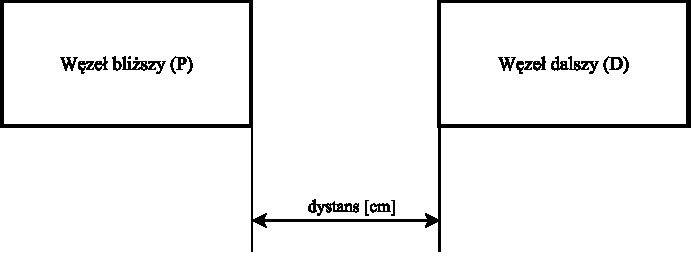
\includegraphics[width=0.618\linewidth]{per_two_nodes.pdf} 
	\caption{Dystans pomiędzy węzłami dla sieci dwóch mikrokontrolerów}
	\label{rys:two_nodes_setup}
\end{figure}

Wyżej wymienione odległości stosowano również w przypadku kolejnego badanego parametru, tj. ilości węzłów
składających się na sieć BLE. W celu łatwej identyfikacji węzłów, wprowadza się następujące nazewnictwo:
\begin{itemize}
	\item węzeł bliższy (ang./łac. \textit{proximal node}/\textit{nodus proximalis}) - węzeł będący połączony bezpośrednio
	ze stacją akwizycji danych i kontroli przepływu eksperymentu.
	\item węzeł środkowy (ang./łac. \textit{intermedial node}/\textit{nodus [inter]medius}) - węzeł działający w trybie
	przekaźnika (terminologia Mesh: \textit{Relay}). Węzeł ten nie uczestniczy bezpośrednio w badaniach tj. nie są
	z niego odczytywane jakiekolwiek dane.
	\item węzeł dalszy (ang./łac. \textit{distal node}/\textit{nodus distalis}) - węzeł zliczający ilość odebranych danych \textit{r},
	udostępniający jednocześnie usługę umożliwiającą odczyt tych wartości tak jak opisano to w podrozdziale \ref{prep:uc-software}.
\end{itemize}

Postanowiono o równoodległym rozstawieniu węzłów - Rysunek~\ref{rys:three_nodes_setup}. Dla sieci 3 węzłów,
maksymalna odległość dzieląca węzeł bliższy od węzła dalszego to 42m. Protokół badawczy zawiera informację 
tylko o odległości w~rozumieniu równoodległego rozstawienia węzłów. Odległość pomiędzy elementami 
jest oczywistą operacją arytmetyczną.

\begin{figure}[!ht]
	\centering 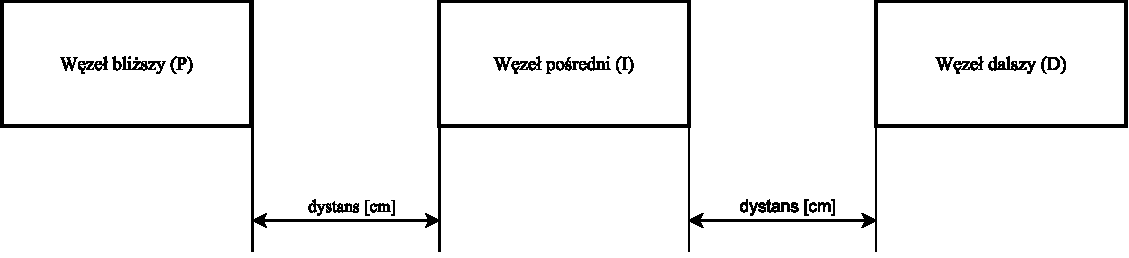
\includegraphics[width=0.99\linewidth]{per_three_nodes.pdf} 
	\caption{Dystans pomiędzy węzłami dla sieci trzech mikrokontrolerów}
	\label{rys:three_nodes_setup}
\end{figure}

Odległość pomiędzy węzłami mierzona jest z użyciem taśmy mierniczej z podziałką 1mm. Tolerancję pomiarów należy
przyjąć jako najdłuższy wymiar zestawu uruchomieniowego P-NUCLEO-WB55 - 70mm \cite{stmicroelectronics_um2435_2019}.
Pomiar odbywał się na płasko, mierząc odległość pomiędzy leżącymi na glebie węzłami. Błędy pomiarowe wynikłe
z ukształtowania terenu są prawdopodobne i~wynikają z~terenowego charakteru badań.

W celu zminimalizowania ryzyka pojawienia się losowych błędów o nieznanym pochodzeniu badanie powtarzano pięciokrotnie,
w sposób następujący: dla wybranego środowiska, ilości węzłów i zadanej odległości pomiędzy węzłami, wykonaj
5 powtórzeń pomiarowych dla każdego z zadanych interwałów pomiarowych.

\begin{equation}
\label{experiment_definition}
\exists e, \exists n, \exists d: PER_i = f(e, n, d), i=1,...,5
\end{equation}

gdzie:

\begin{description}
\item[e] - środowisko
\item[n] - ilość węzłów
\item[d] - równoodległy dystans pomiędzy węzłami
\item[i] - ilość powtórzeń
\item[PER] - Packet Error Rate dla wybranego powtórzenia przy stałych parametrach e, n, d
\end{description}

Wykorzystując tak zebrane dane, wyrysowano je na szeregu wykresów wyznaczając jednocześnie
linie aproksymacyjne z użyciem modelu liniowego wyznaczonego metodą najmniejszych kwadratów. Odchylenia standardowe zaprezentowane
są z użyciem ograniczonego tła otaczającego linię w tym samym kolorze o~zmienionym parametrze nieprzezroczystości.

Parametry transmisji danych nie ulegały zmianie podczas przeprowadzanych doświadczeń. Poniższe wartości należy
przyjąć za stałe:
\begin{itemize}
\item Szybkość transmisji: 2Mbps
\item Moc transmisji danych: 0dBm
\end{itemize}

%%%%%%%%%%%%%%%%%%%%%%%%%%%%%%%%%%%%%%%%%%%%%%%%%%%%%%%%%%%%%%%%%%%%%%%%%%%%%%%%
%% SUBSECTION: Zależność \gls{PER} względem częstości zapytań
%%%%%%%%%%%%%%%%%%%%%%%%%%%%%%%%%%%%%%%%%%%%%%%%%%%%%%%%%%%%%%%%%%%%%%%%%%%%%%%%
\subsection{Zależność PER względem częstości zapytań}

Pierwszą sprawdzaną hipotezą jest empiryczna weryfikacja czy częstość zapytań wpływa na \gls{PER}.
W tym celu wykreślono szereg wykresów dla wybranych interwałów czasowych. Pozostałe parametry traktowane są
jako stałe.

Rysunek~\ref{rys:per_to_distance_under_100ms} przedstawia zależność PER dla interwału 100 milisekund w~zależności
od odległości dla sieci złożonej z dwóch i trzech węzłów. 

\begin{figure}[!htb]
	\centering 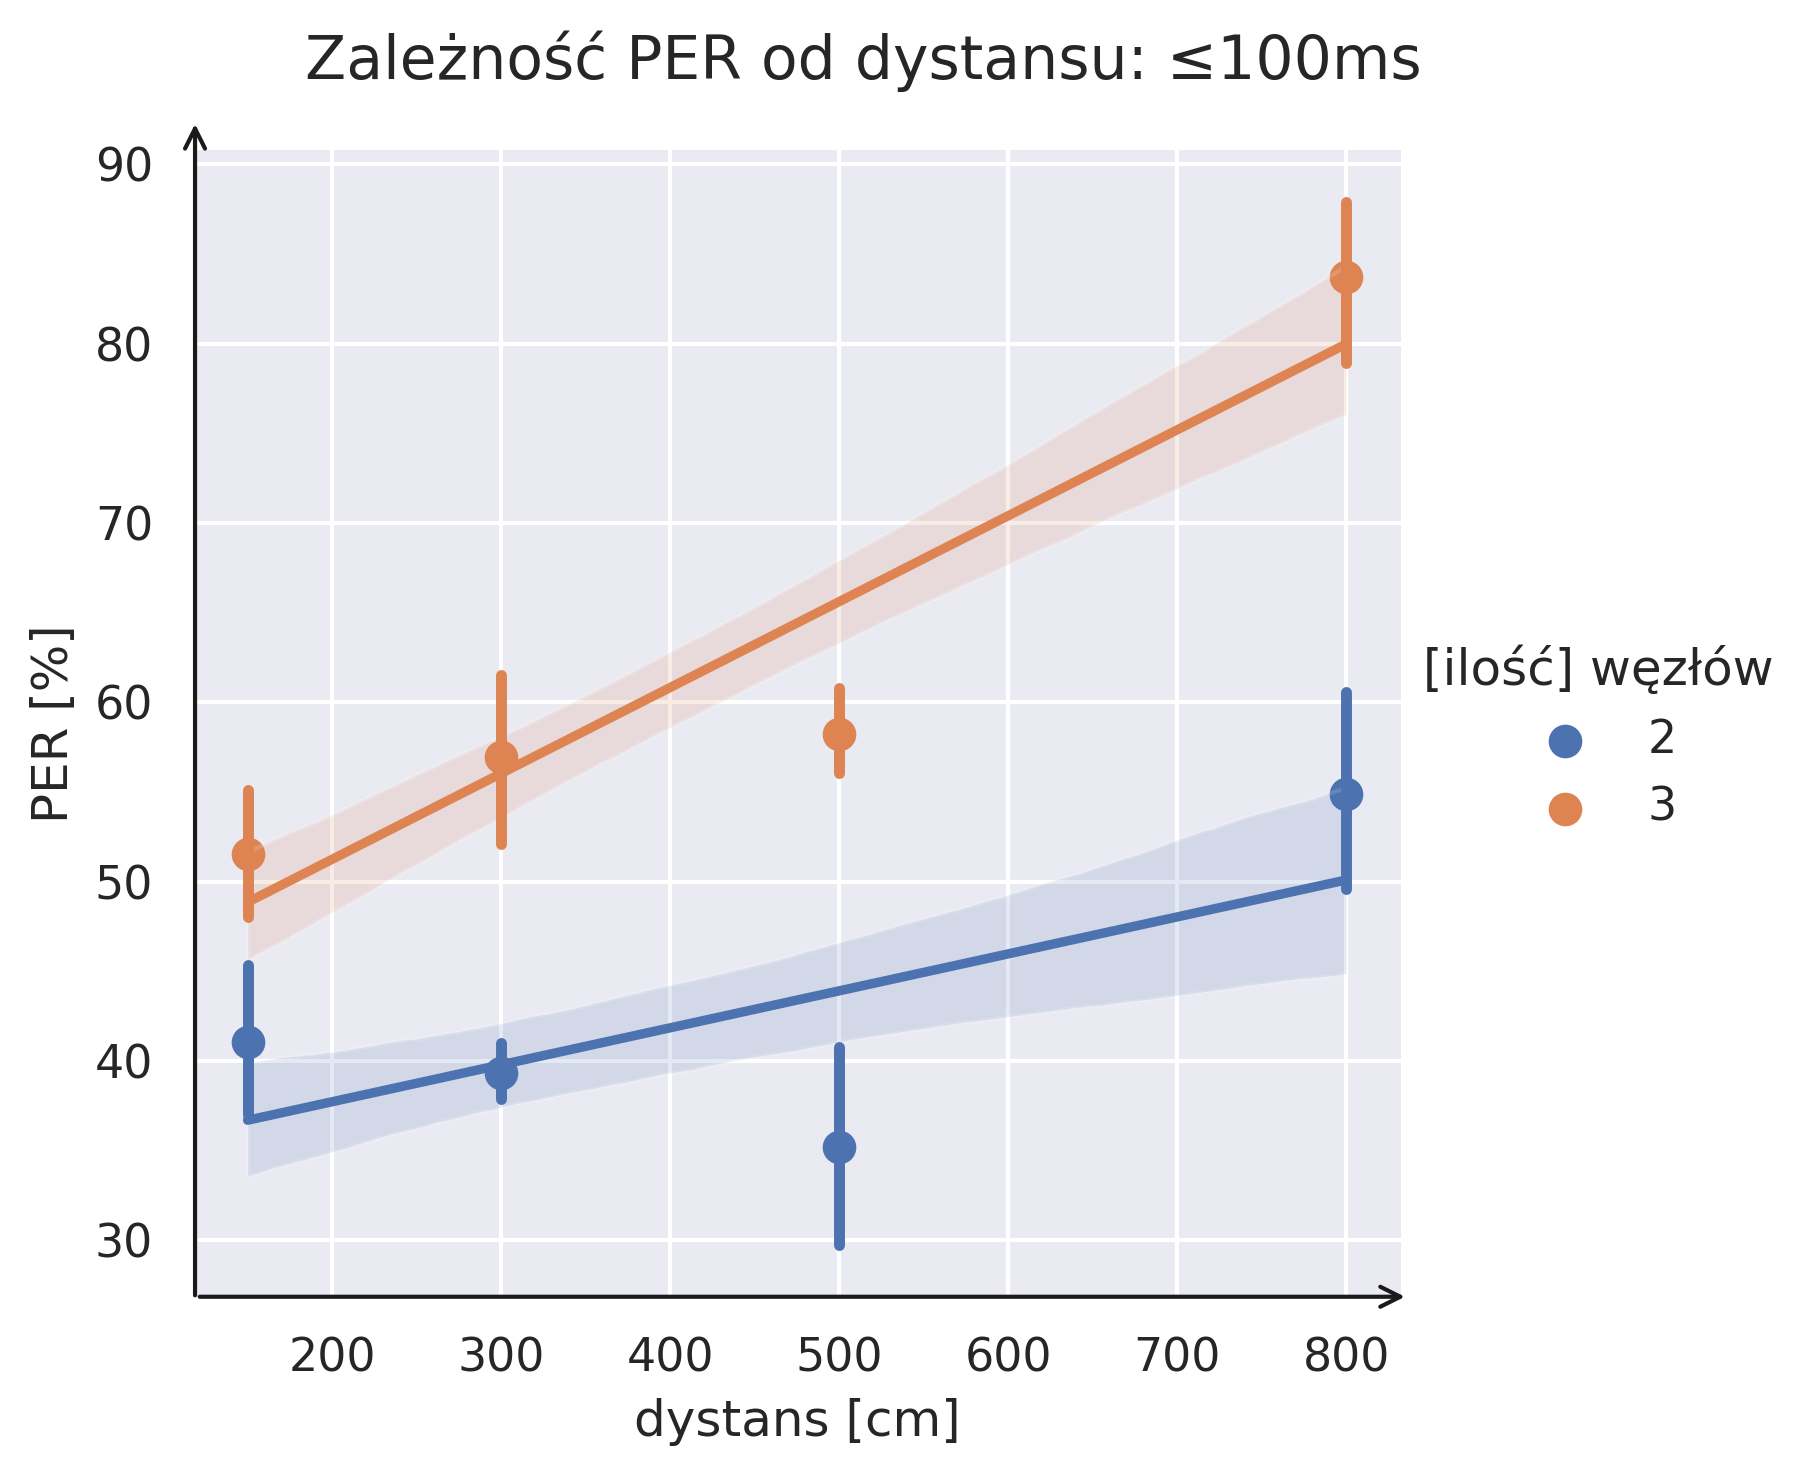
\includegraphics[width=0.618\linewidth]{per_to_distance_under_100ms.png}
	\caption{Zależność \gls{PER} od dystansu dla zapytań o częstości $\leqslant$ 100ms dla różnej liczby węzłów}
	\label{rys:per_to_distance_under_100ms}
\end{figure}

Niewątpliwą cechą ukazanych danych jest wysoka wartość PER już przy tak niewielkiej odległości jak 150 cm pomiędzy węzłami.
Utrata 40-50\% wysyłanych pakietów danych już na pierwszym dystansie pomiarowym może być spowodowana wieloma czynnikami.
Przypuszczalnie, wpływ na taki rezultat wywodzi się z czynników środowiskowych lub ze sposobu wykonywania 
eksperymentu. Niewykluczone są również ograniczenia sprzętowe.

Wraz ze wzrostem odległości pomiędzy węzłami PER wzrasta pomimo wysokiej wartości początkowej. Jest to 
oczekiwana zależność i zgodna z wiedzą techniczną.

Prowadząc dalszą analizę zależności PER od częstości zapytań, sprawdzono wpływ środowiska na jakość transmisji danych.
Rysunek~\ref{rys:per_to_distance_under_100ms_different_envs} przedstawia wybraną zależność. Rozróżnienie
na ilość węzłów nie zostało tutaj uwzględnione. Pomiary przeprowadzone w~najbliższym dobranym dystansie ponownie 
wskazują na 40-50\% utratę pakietów w węźle dalszym. Analogiczne rezultaty obserwowane są na pozostałych dystansach 
z~oczekiwaną tendencją wzrostową.
Wykres dodatkowo przedstawia pewną różnicę w jakości transmisji danych w~zależności od środowiska. Różnica ta 
jednak mieści się w odchyleniu standardowym, posiadając część wspólną dla zadanych parametrów. Nie jest to 
wystarczające do stwierdzenia jednoznacznego wpływu środowiska.

\begin{figure}[!htb]
	\centering 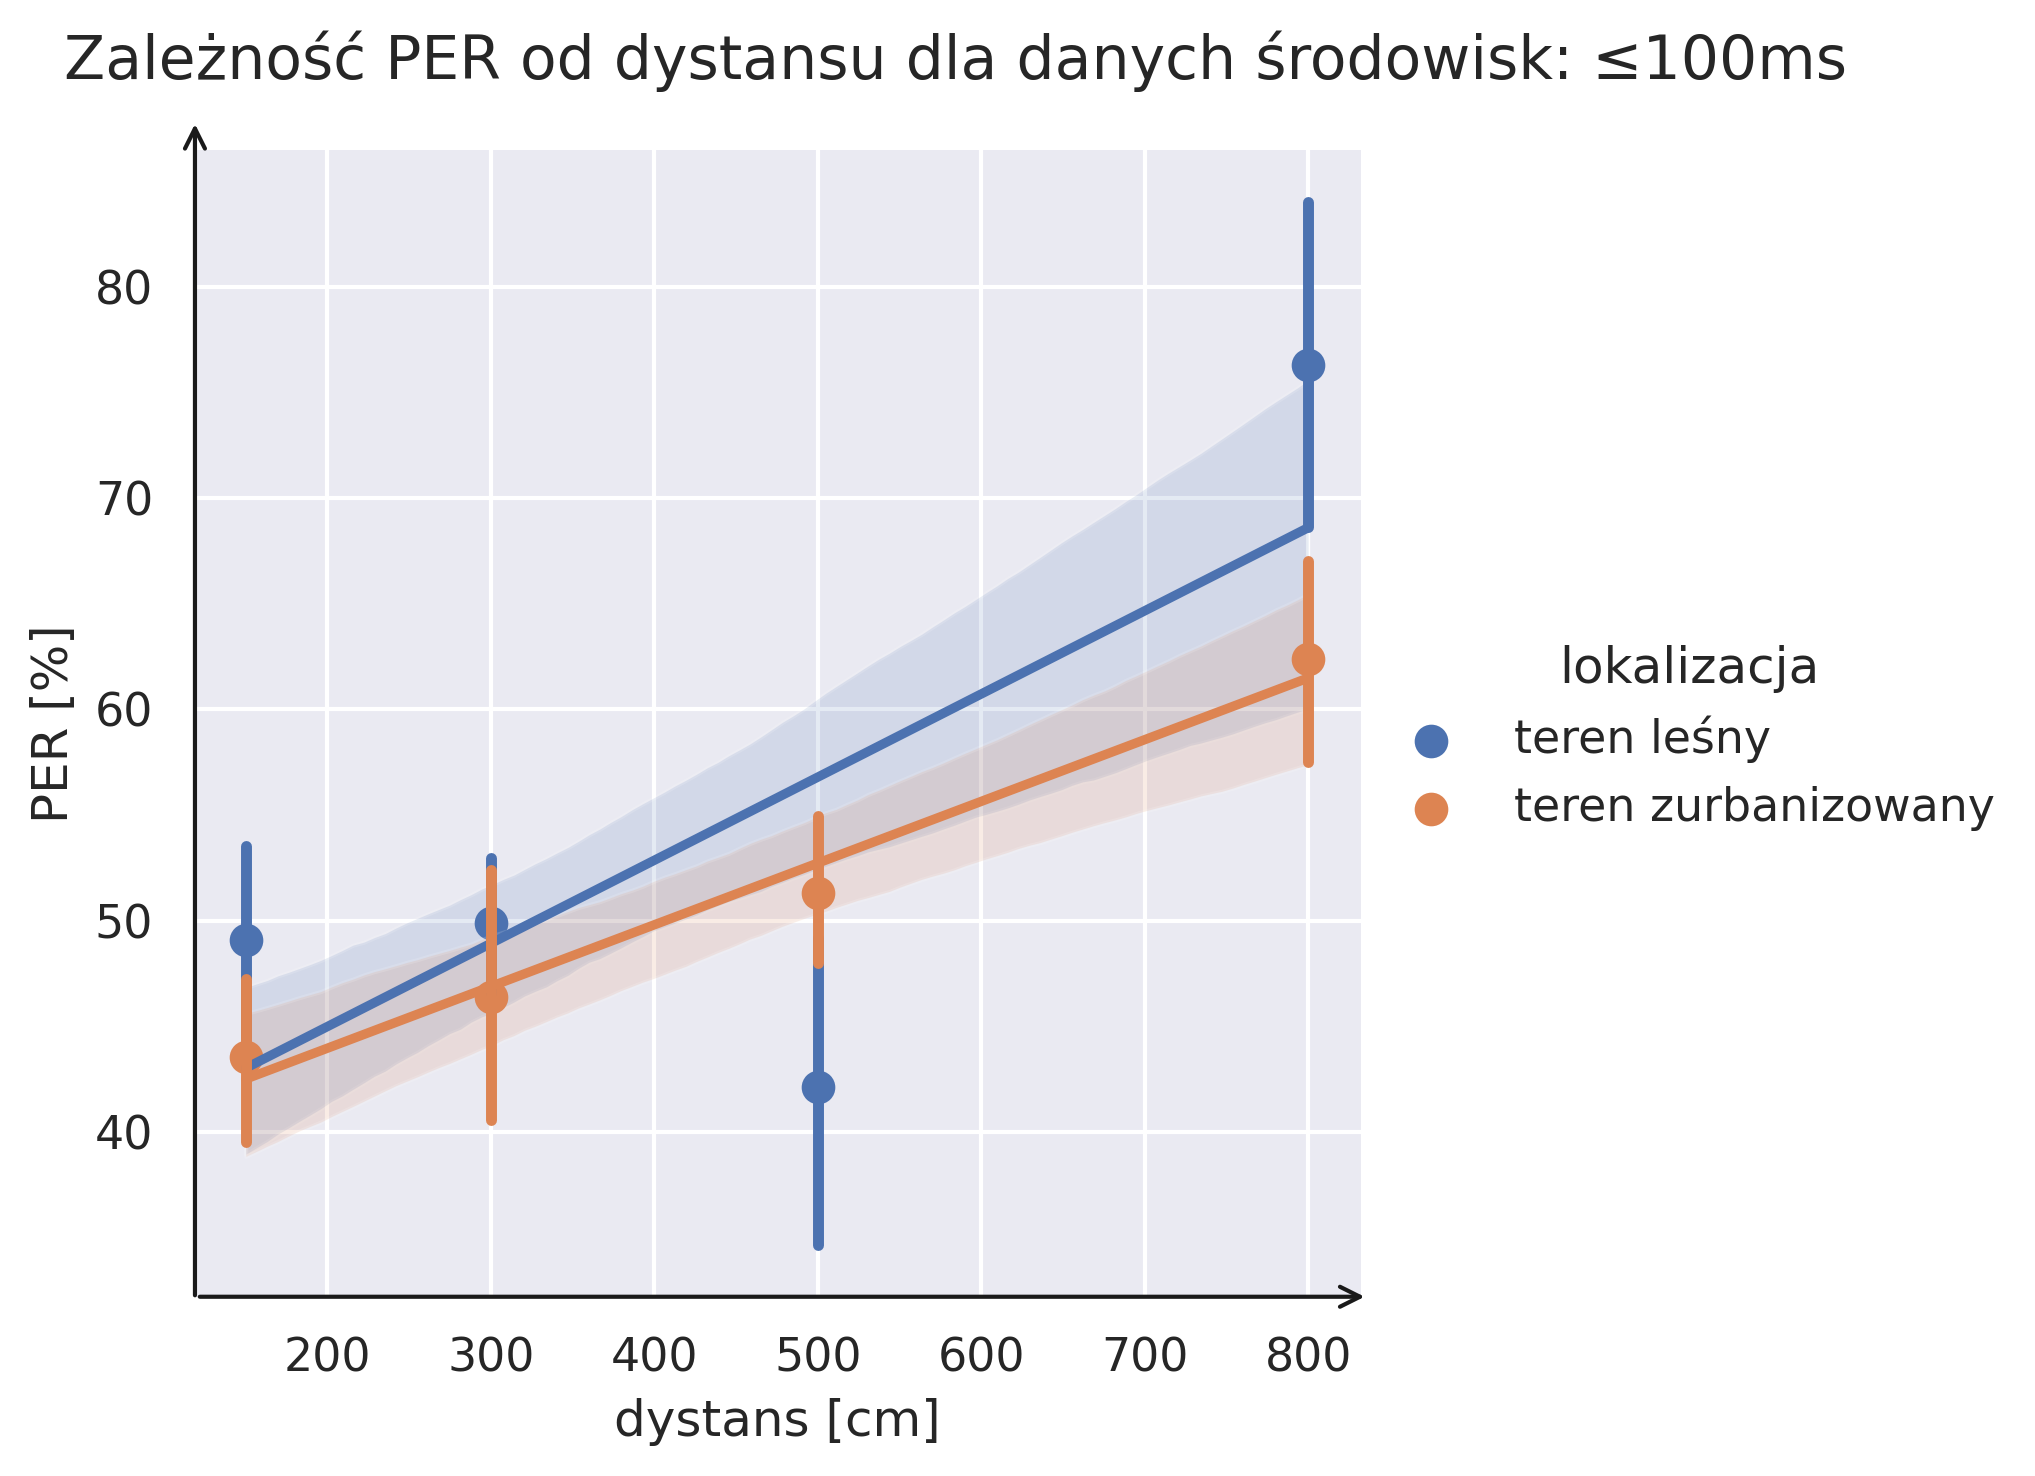
\includegraphics[width=0.618\linewidth]{per_to_distance_under_100ms_different_envs.png} 
	\caption{Zależność \gls{PER} od dystansu dla zapytań o częstości $\leqslant$ 100ms w wybranych środowiskach bez rozróżnienia na liczbę węzłów}
	\label{rys:per_to_distance_under_100ms_different_envs}
\end{figure}

Zestawiając ze sobą wymienione wcześniej czynniki, obserwuje się interesujące zależności. Rysunek~\ref{rys:per_to_distance_under_100ms_different_envs_and_nodes} wskazuje na zależność dystansu, ilości węzłów i rodzaju
środowiska dla wybranego interwału zapytań 100 milisekund. Po raz kolejny obserwowany jest PER wynoszący
40-50\%, niezależnie od środowiska czy ilości węzłów. Sugeruje to wpływ samej testowanej platformy
na ostateczny rezultat. Prawdopodobną hipotezą jest niewystarczająca wielkość zaalokowanych
buforów obsługujących transmisję danych. Mikrokontroler nie będąc w stanie obsłużyć tak częstej transmisji
może doświadczyć awarii, co zaobserwowano podczas badań. Awaria objawiała się brakiem reakcji węzła bliższego
na jakiekolwiek komendy AT, co wymagało ponownego uruchomienia urządzenia. Weryfikacja tego zagadnienia
wymagałaby zaangażowania zaawansowanych narzędzi programistycznych ingerujących m.in. w~pamięć urządzenia.
Niniejsza praca nie podejmuje się wyjaśnienia przyczyn obserwowanych anomalii w działaniu mikrokontrolera,
udostępniając jednocześnie możliwy punkt dla dalszych prac badawczych z zakresu BLE Mesh.

Wpływ samego stosu łączności na PER przy zadanej częstości zapytań zdaje się potwierdzać wykres uwzględniający
jakość transmisji dla dwóch węzłów. Niemalże pozioma linia aproksymacji sugeruje niewielki wpływ dystansu na PER.
Dotyczy to zarówno terenu zurbanizowanego jak i~terenu leśnego. Zbliżone rezultaty zdają się wykluczać
czynniki zewnętrzne.

Interesującą zależnością jest nachylenie wykresu względem osi odciętych. Dla przypadku dwóch węzłów sieci,
połączenie bezpośrednio między węzłami, PER jest niemal stałe na wybranych odległościach, porównywalne
z~przypadkiem terenu leśnego. W przypadku trzech
węzłów, uwidacznia się potencjalny wpływ węzła środkowego, przekazującego pakiety z punktu bliższego do
dalszego. Wraz ze wzrostem dystansu, rośnie wartość PER sięgając nawet 90\% w terenie leśnym. Różne nachylenie
dla wybranych środowisk również sugeruje znaczący wpływ środowiska na PER.

\begin{figure}[!htb]
	\centering 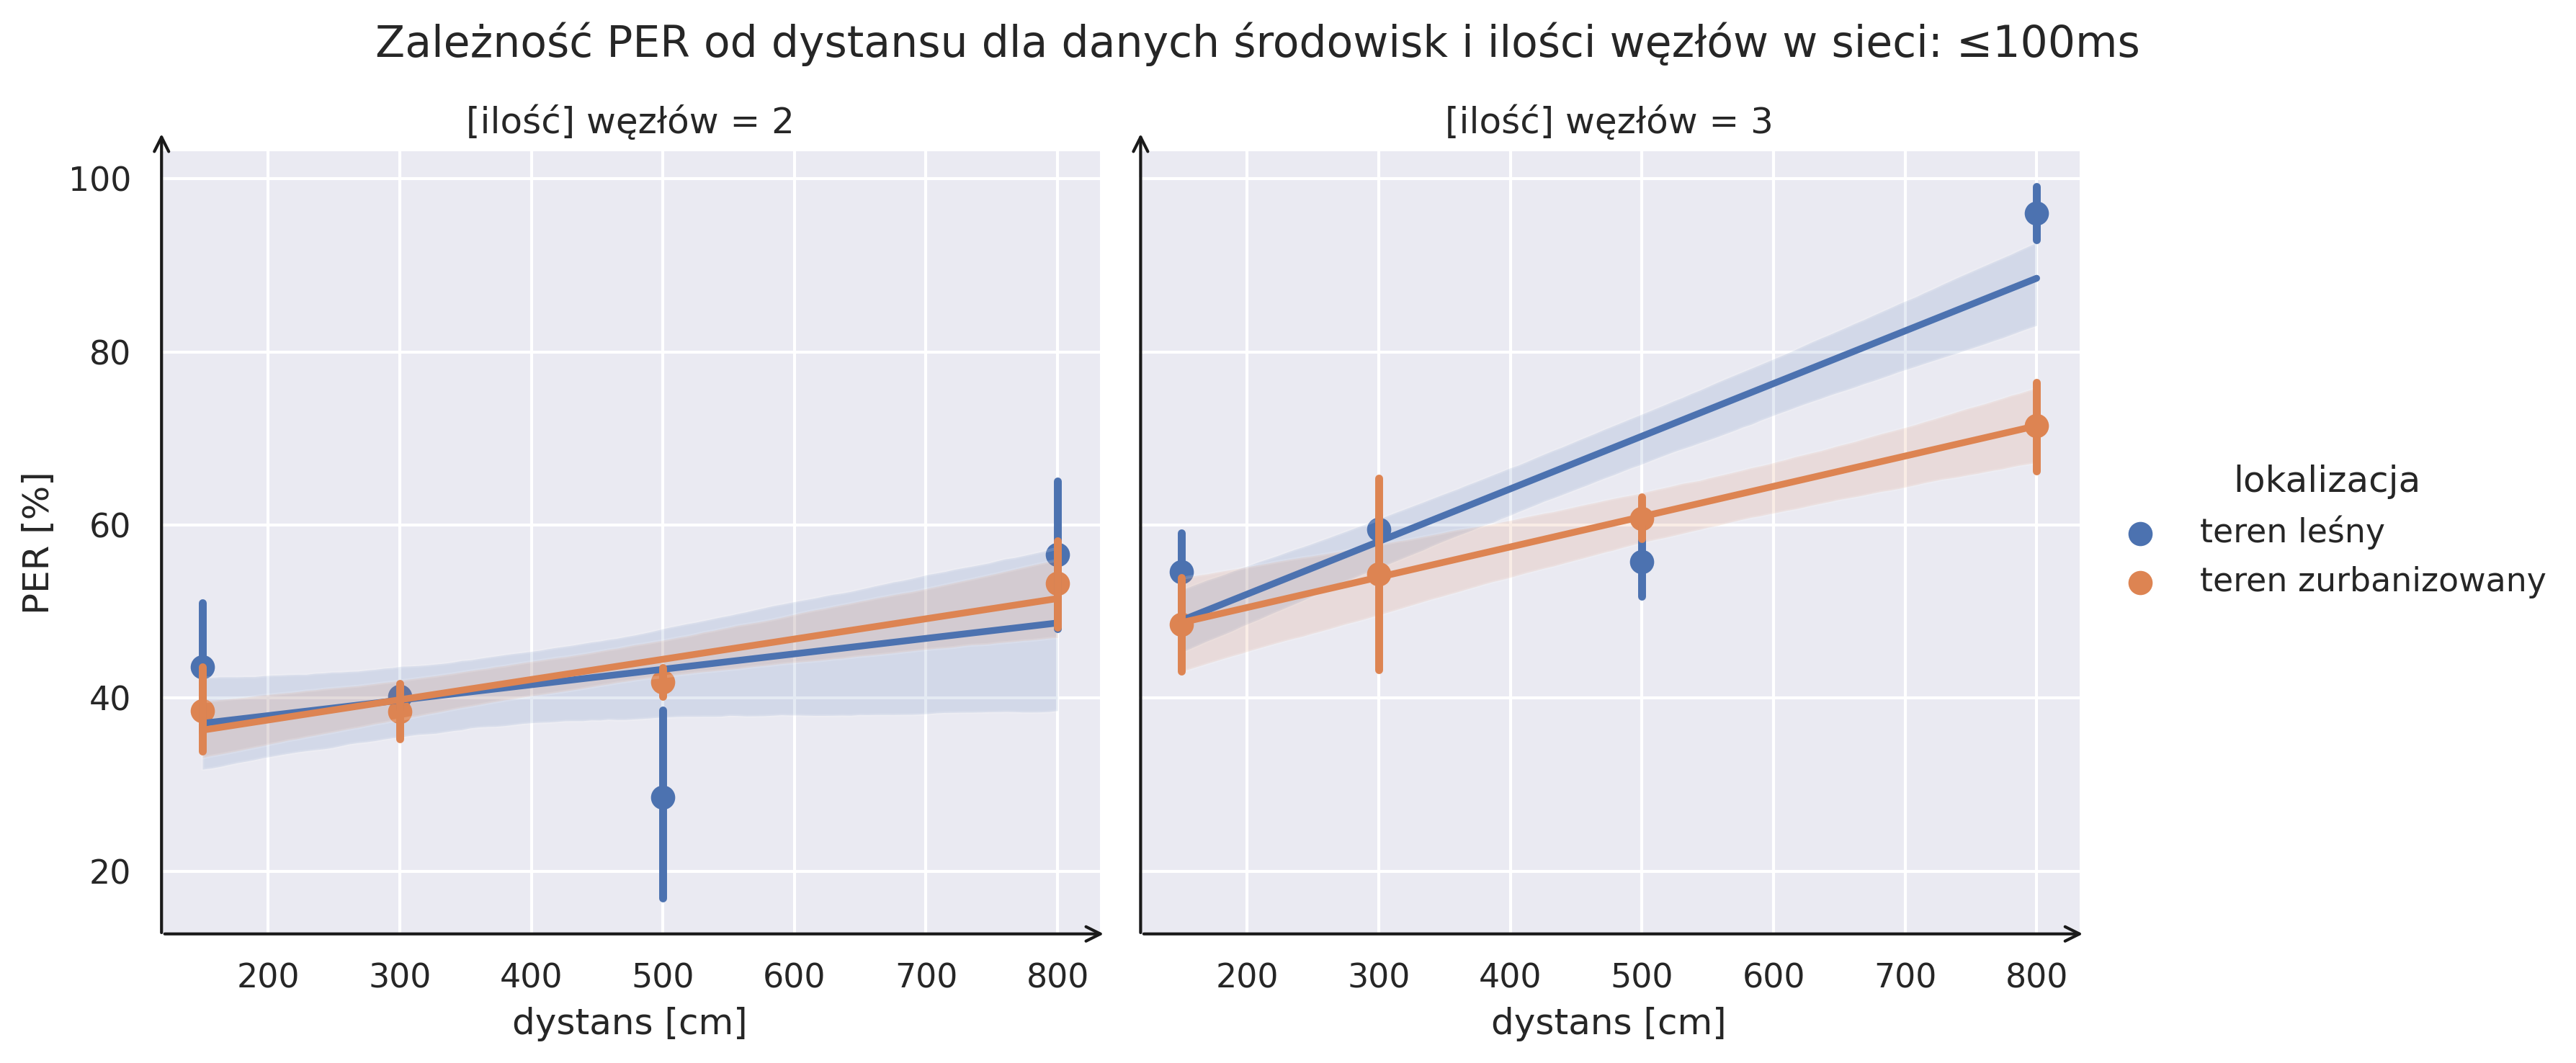
\includegraphics[width=0.99\linewidth]{per_to_distance_under_100ms_different_envs_and_nodes.png}
	\caption{Zależność \gls{PER} od dystansu dla zapytań o częstości $\leqslant$ 100ms w wybranych środowiskach i liczbę badanych węzłów}
	\label{rys:per_to_distance_under_100ms_different_envs_and_nodes}
\end{figure}

Znając charakterystykę łączności dla okresów poniżej 100 milisekund, weryfikuje się pozostałe wybrane częstości, zgodnie
z podanymi wartościami~\ref{items:ping_intervals}. Rysunek~\ref{rys:per_to_distance_over_100ms_different_envs_different_ping_interval}
prezentuje pozostałe interwały w zależności od dystansu i wybranych środowisk bez rozróżnienia na ilość węzłów w sieci.

Przeprowadzone pomiary w terenie leśnym wskazują charakterystykę połączenia zgodną z~intuicyjnymi przewidywaniami.
Na~początkowym dystansie 150cm nie obserwuje się problemów z łącznością. Wszystkie wysłane pakiety zostały
odebrane przez węzeł dalszy. Kolejny dystans wskazuje już na pewną utratę pakietów poniżej 20\%. Prawdopodobnym czynnikiem
jest pogoda lub ukształtowanie terenu leśnego. Co istotne, pomiary dla różnych interwałów odpytywań są zbliżone.
Sugerowałoby to brak wpływu częstości na \gls{PER}. Na pozostałych dystansach pomiarowych, wartości utraty pakietów
są do siebie wzajemnie zbliżone osiągając swoje maksimum na dystansie 21m - blisko 100\% zaginionych pakietów.

Charakterystyka łączności w terenie zurbanizowanym prezentuje się podobnie. Nie obserwuje się znaczącej utraty 
pakietów na względnie bliskich dystansach (150, 300 i 500cm). Wartość PER rośnie wraz ze wzrostem odległości
pomiędzy węzłami osiągając w swoim szczycie wartość ok. 40\%. Co istotne, linie aproksymacyjne są do siebie
zbliżone, ponownie sugerując brak korelacji pomiędzy częstością wysyłania komunikatów a~wartością PER.


\begin{figure}[!htb]
	\centering 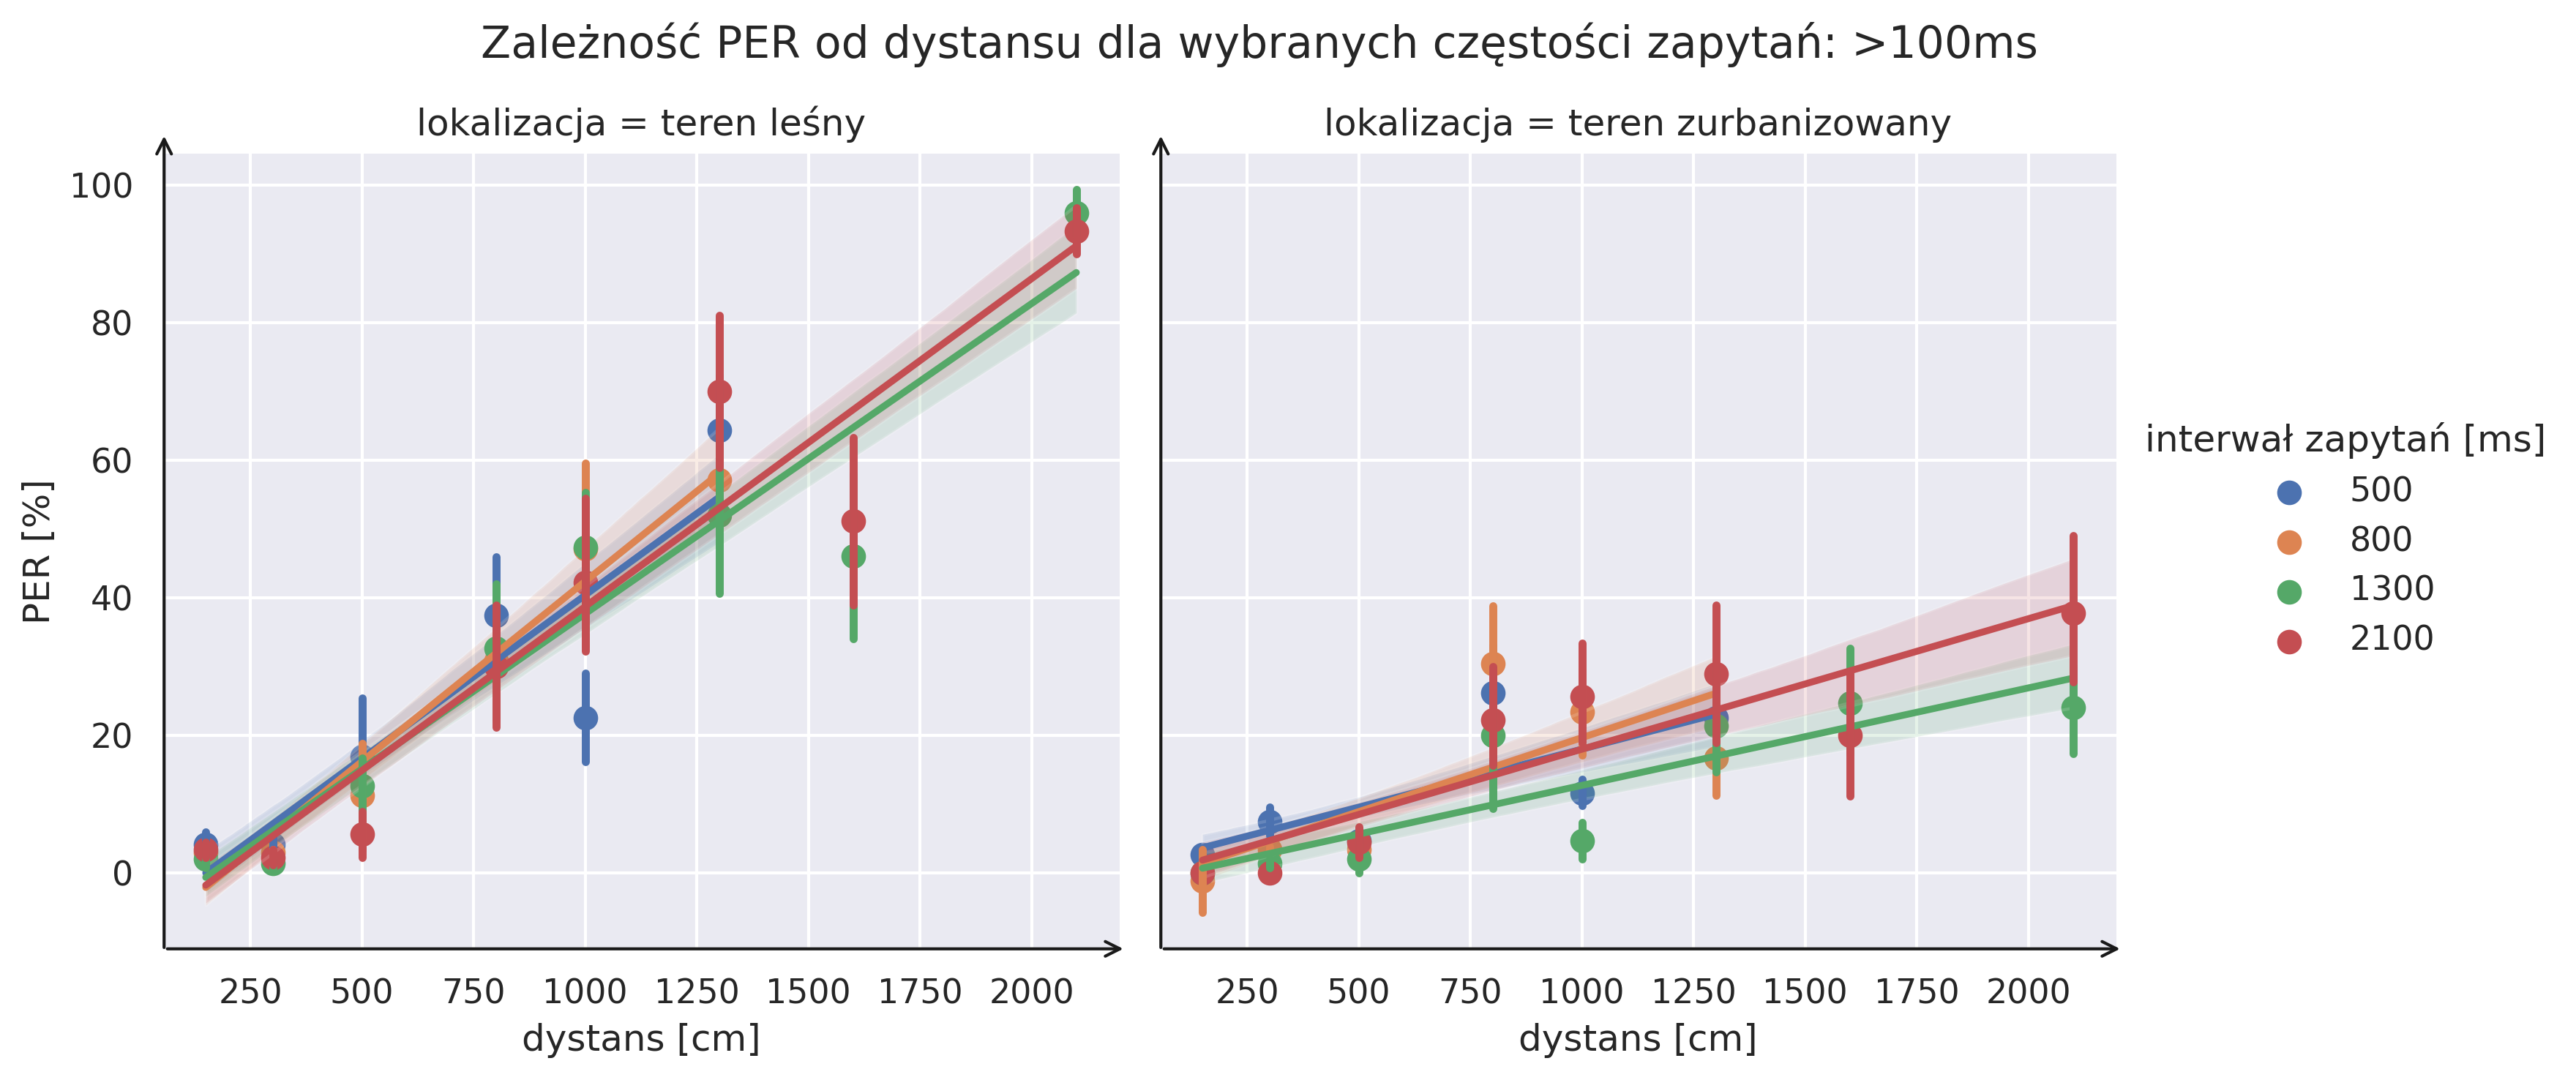
\includegraphics[width=0.99\linewidth]{per_to_distance_over_100ms_different_envs_different_ping_interval.png} 
	\caption{Zależność \gls{PER} od dystansu dla zapytań o częstości >100ms w wybranych środowiskach}
	\label{rys:per_to_distance_over_100ms_different_envs_different_ping_interval}
\end{figure}

Zależność pomiędzy PER a częstością odpytywań została zbadana wykorzystując narzędzia statystyczne. Traktując model
liniowy, jak sugerują zaprezentowane wykresy, tworzonych zgodnie z~metodą najmniejszych kwadratów wylicza się 
współczynnik determinacji dla następujących zmiennych niezależnych: dystans oraz PER. W~kolejnym kroku uwzględnia
się fakt wykorzystywania korelacji wielu zmiennych, dostosowując odpowiednio wartość.


\begin{table}[!ht]
\centering
	\begin{tabular}{p{4.5cm}|r|r}
	Środowisko              & $R^2$             & $R^2_{dostosowany}$\\\hline
	Teren leśny             & 0.04958           & 0.04272\\\hline
	Teren zurbanizowany     & 0.04887           & 0.04200\\\hline
	\end{tabular}
\caption{\label{tab:corr_between_ping_intervals}Współczynnik determinacji dla zależności interwału zapytań od dystansu i~PER w~wybranych środowiskach}
\end{table}

Ostatecznie, otrzymany współczynnik determinacji przyjmujący wartość $R^2=0,04-0,05$.  Istnieje 4\%-owy wpływ
interwału zapytań o częstościach większych niż 100 milisekund na ostateczny rezultat PER. Pozwala to
wykluczyć ten czynnik wykluczyć z dalszych rozważań uznając go za marginalny.

%%%%%%%%%%%%%%%%%%%%%%%%%%%%%%%%%%%%%%%%%%%%%%%%%%%%%%%%%%%%%%%%%%%%%%%%%%%%%%%%
%% SUBSECTION: Zależność \gls{PER} względem odległości między węzłami
%%%%%%%%%%%%%%%%%%%%%%%%%%%%%%%%%%%%%%%%%%%%%%%%%%%%%%%%%%%%%%%%%%%%%%%%%%%%%%%%
\subsection{Zależność PER względem odległości między węzłami}

Ustaliwszy brak (pomijalnie mały) wpływu częstości zapytań (dla częstości wartości >100ms), praca podejmuje dalszą prezentację
danych pod postacią zależności odległości na PER.

Rysunek~\ref{rys:per_to_distance_over_100ms} przedstawia zebrane dane zestawiając odległość i~ilość węzłów składających
się na sieć Mesh. Na początkowych dystansach PER ma wartość bliską bądź równą zeru. Wraz ze wzrostem odległości pomiędzy
węzłami, badany współczynnik rośnie, co jest zgodne z oczekiwaniami. Na dystansie 16m obserwuje się przełamanie
linii aproksymacji. Dodatkowy węzeł środkowy znacząco i pozytywnie wpływa na PER przy kolejnych odległościach
umożliwiając przekazywanie informacji w~sieci. PER w najdalszym punkcie pomiarowym osiąga wartości od ok.~60\% do 70\%.
Należy jednak mieć na uwadze, iż zestawienie nie rozróżnia środowiska w którym następowało zliczanie pakietów.


\begin{figure}[!htb]
	\centering 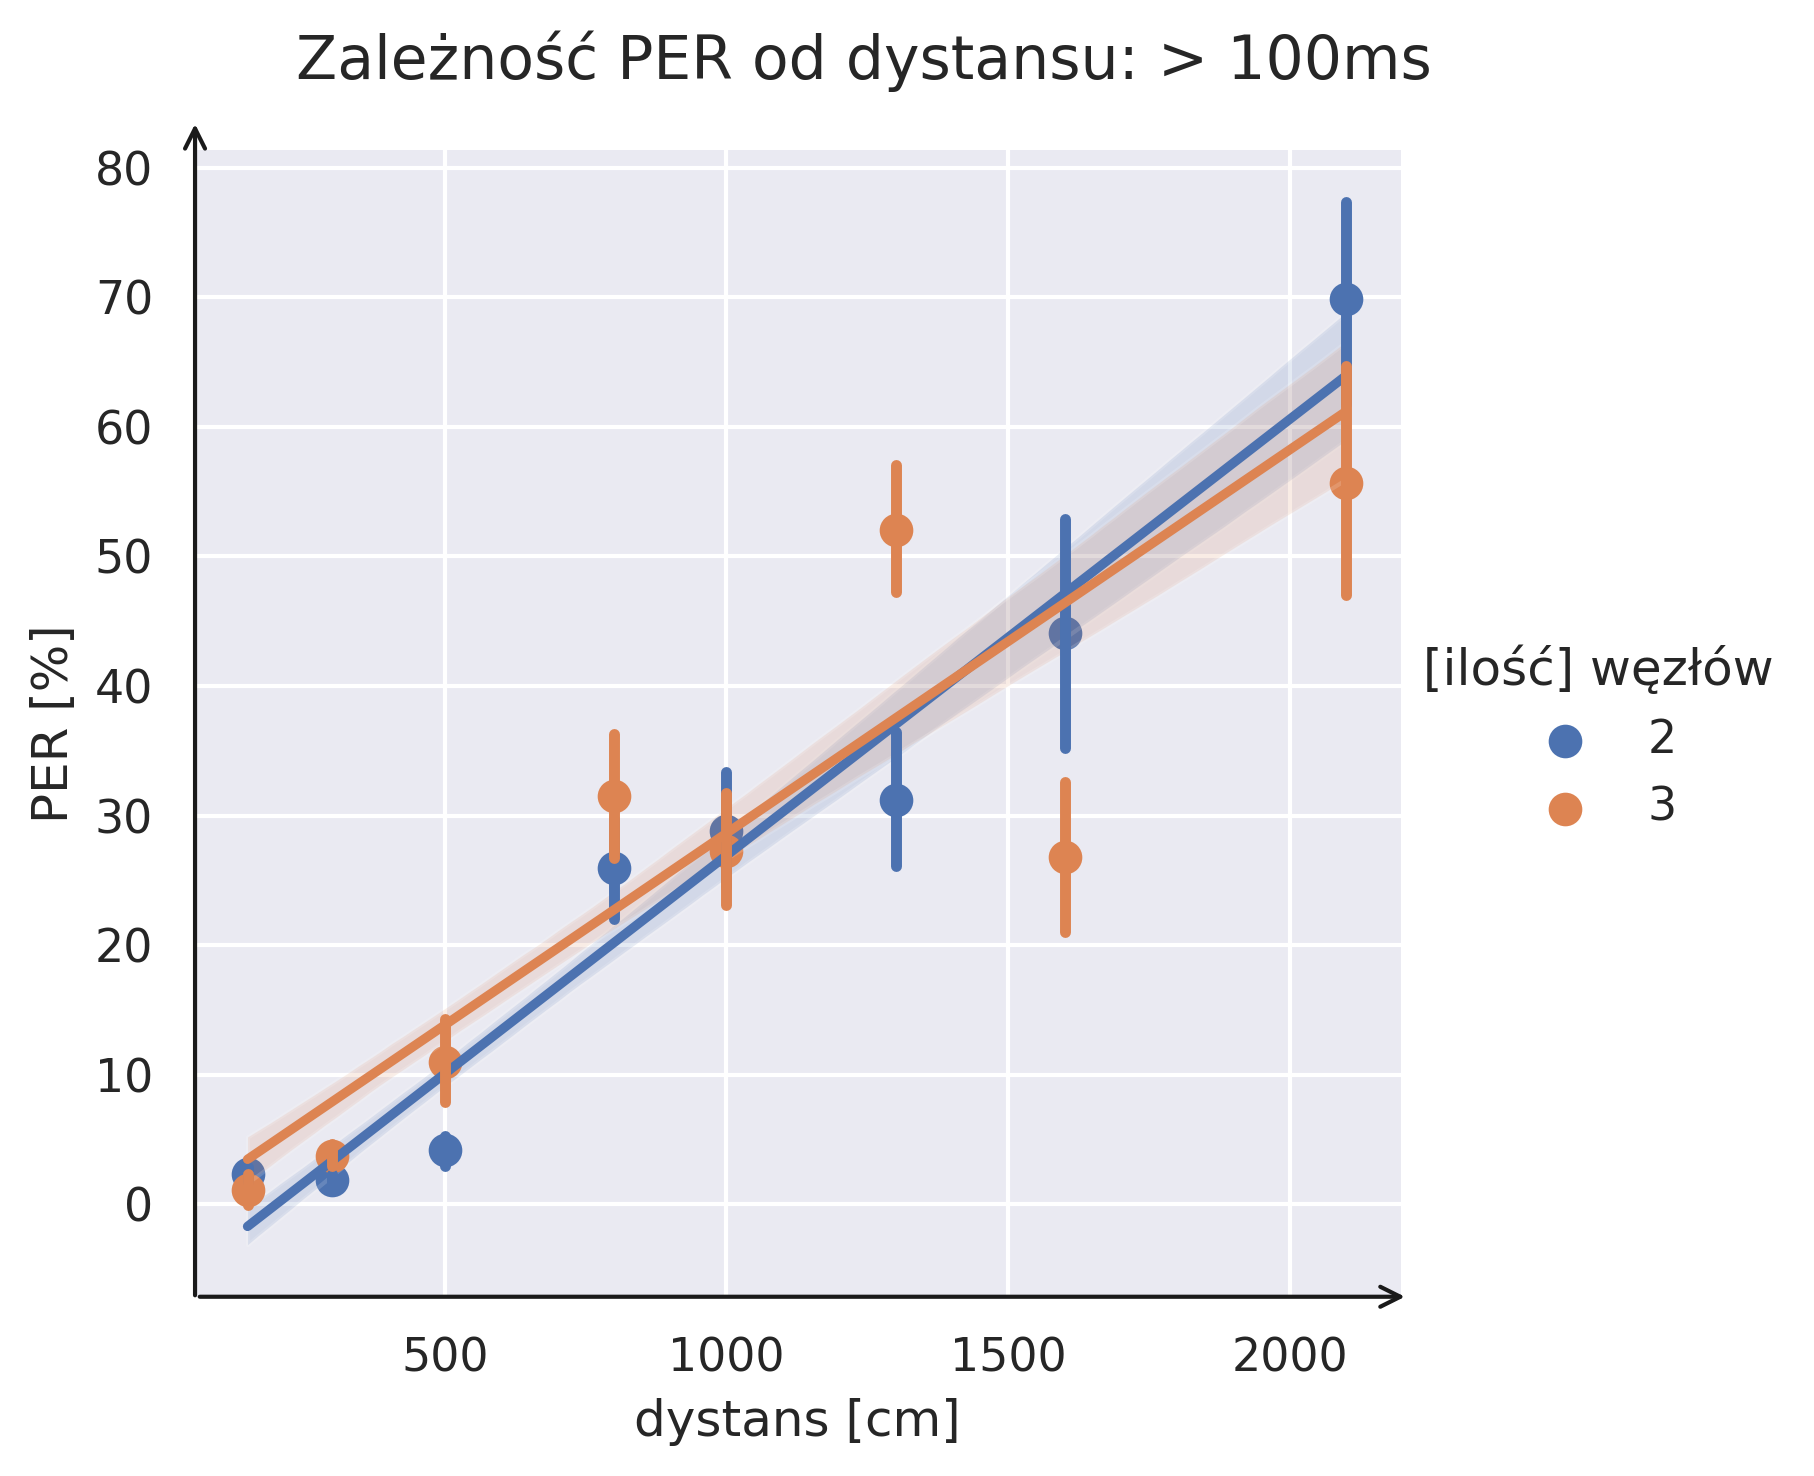
\includegraphics[width=0.618\linewidth]{per_to_distance_over_100ms.png}
	\caption{Zależność \gls{PER} od dystansu dla zapytań o częstości >100ms dla różnej liczby węzłów}
	\label{rys:per_to_distance_over_100ms}
\end{figure}

Rysunek~\ref{rys:per_to_distance_over_100ms_different_envs} uwzględnia wpływ środowiska na PER. Wykres zdecydowanie
wskazuje na różnicę pomiędzy terenem zurbanizowanym a terenem leśnym. Na początkowych dystansach PER jest zbliżone
niezależnie od odległości międzywęzłowych. Znaczące różnice w pomiarach, a dzięki temu również względem linii aproksymacyjnej,
występują już na dystansie 5m. PER w przypadku miejskim jest bliskie zera, gdzie analogiczne pomiary w środowisku
leśnym sugerują piętnastoprocentowy poziom zgubionych pakietów. Wraz ze wzrostem dystansu, wartość PER wzrasta.
Niemniej jednak nachylenie linii wskazuje na zdecydowanie wolniejsze narastanie utraty danych podczas transmisji
bezprzewodowej dla przypadku miejskiego. Na maksymalnym dystansie międzywęzłowym wynoszącym 21m, PER
przybiera wartość ok. 30\%. W analogicznym przypadku dla środowiska leśnego następuje niemal całkowita utrata
transmisji.

\begin{figure}[!htb]
	\centering 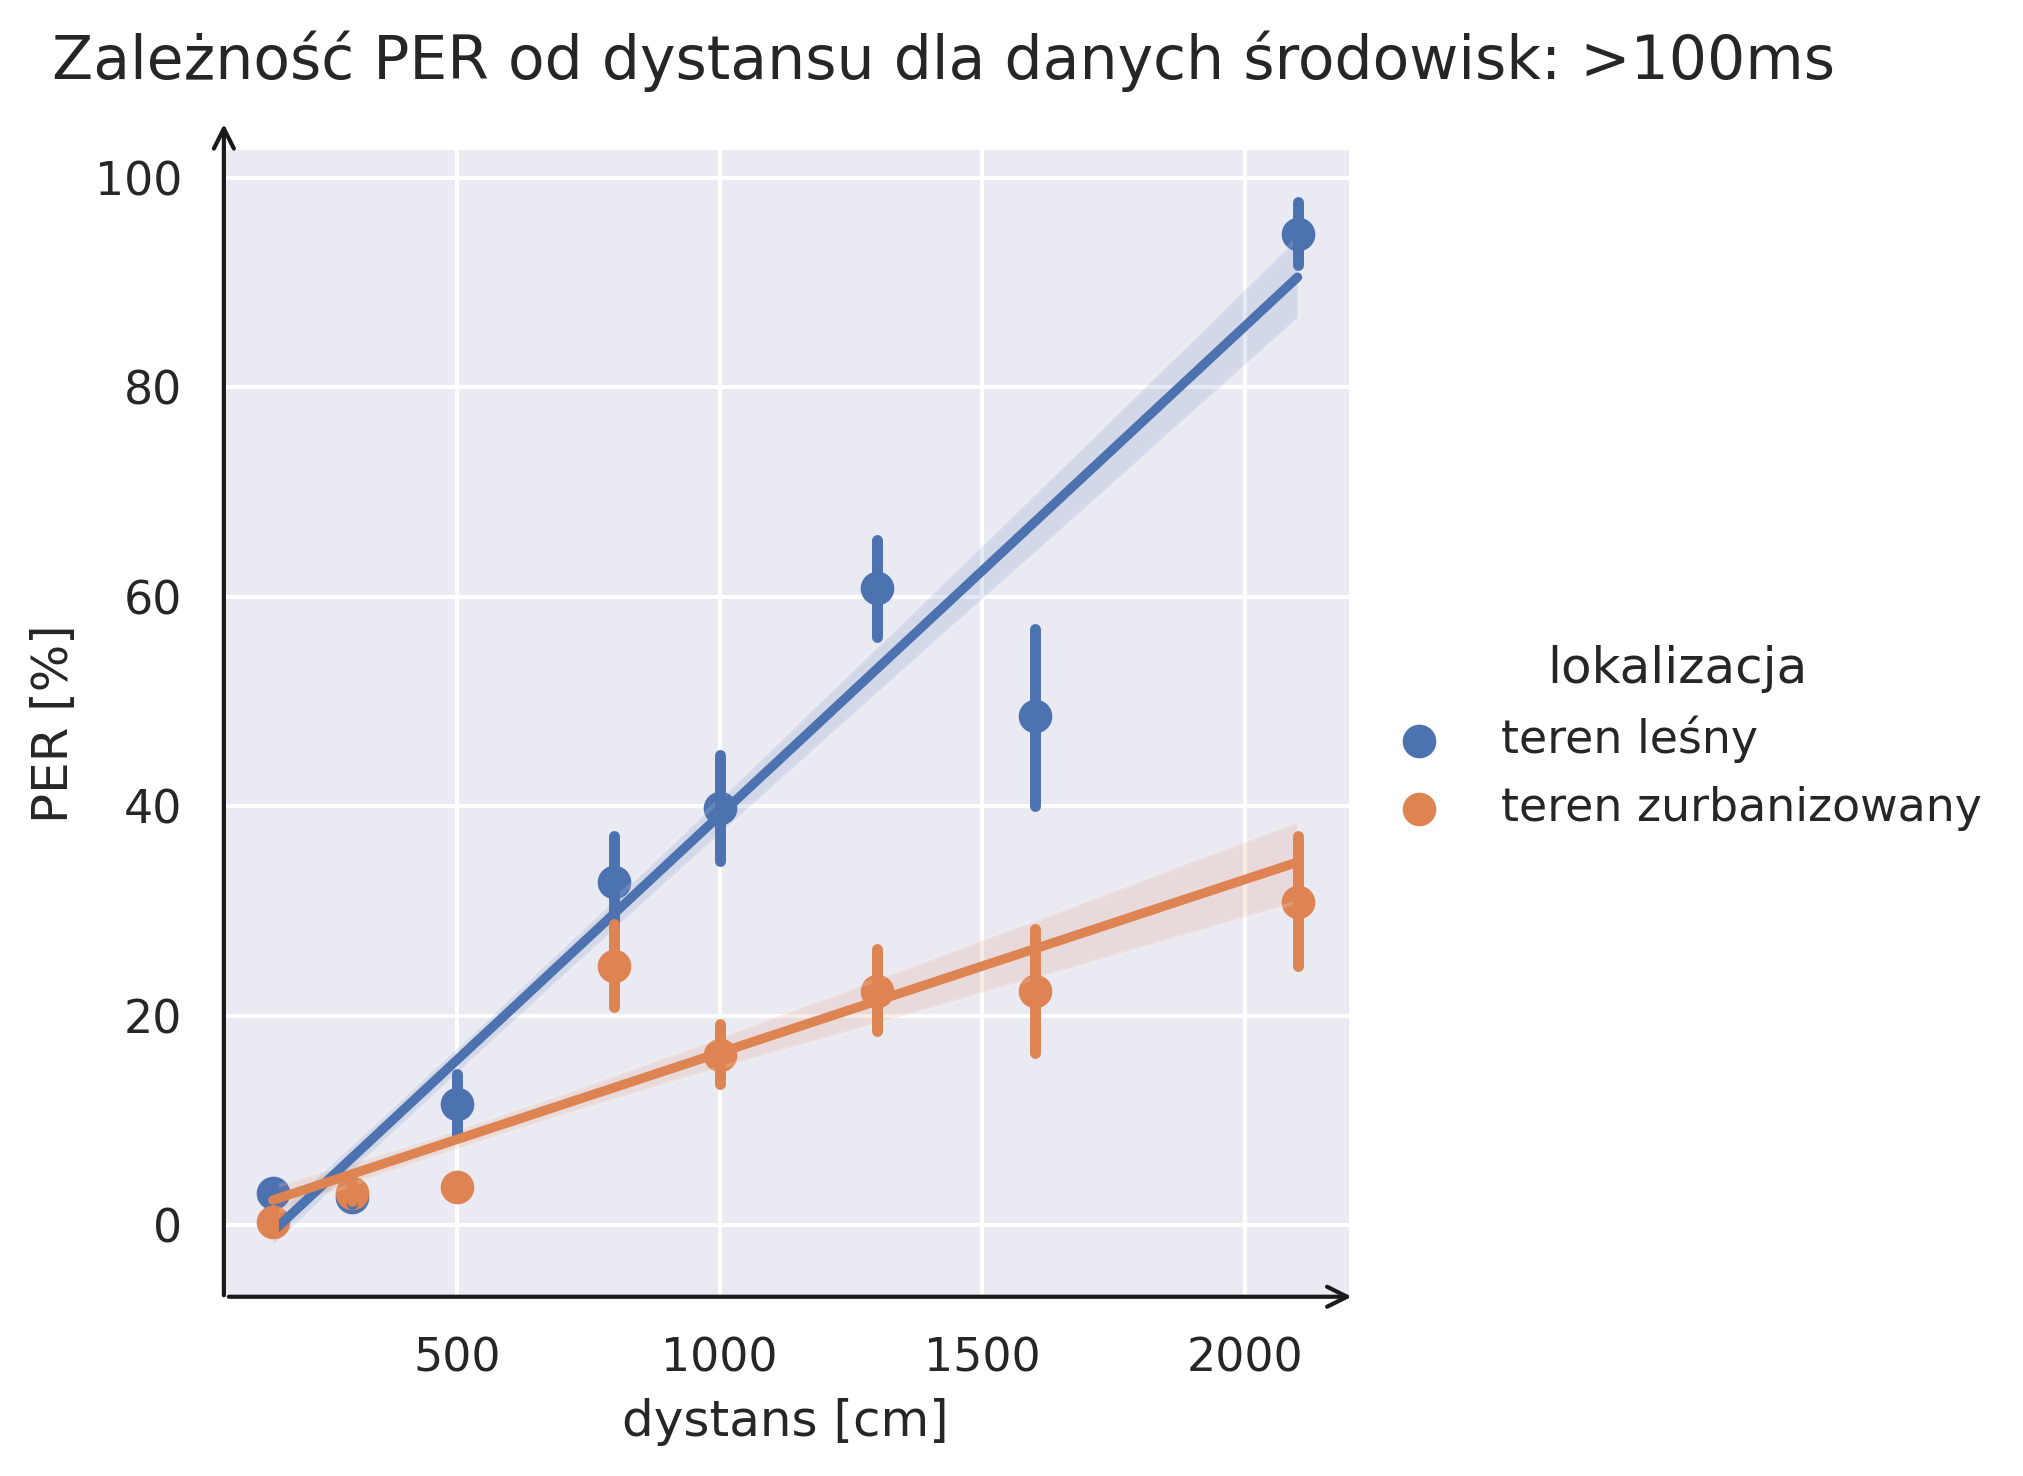
\includegraphics[width=0.618\linewidth]{per_to_distance_over_100ms_different_envs.png} 
	\caption{Zależność \gls{PER} od dystansu dla zapytań o częstości >100ms w wybranych środowiskach bez rozróżnienia na liczbę węzłów}
	\label{rys:per_to_distance_over_100ms_different_envs}
\end{figure}

Ostatnia prezentowana zależność ukazana jest na Rysunku~\ref{rys:per_to_distance_over_100ms_different_envs_and_nodes}.
Przedstawia on zależność PER od dystansu dla wybranych środowisk i liczby węzłów.

\begin{figure}[!htb]
	\centering 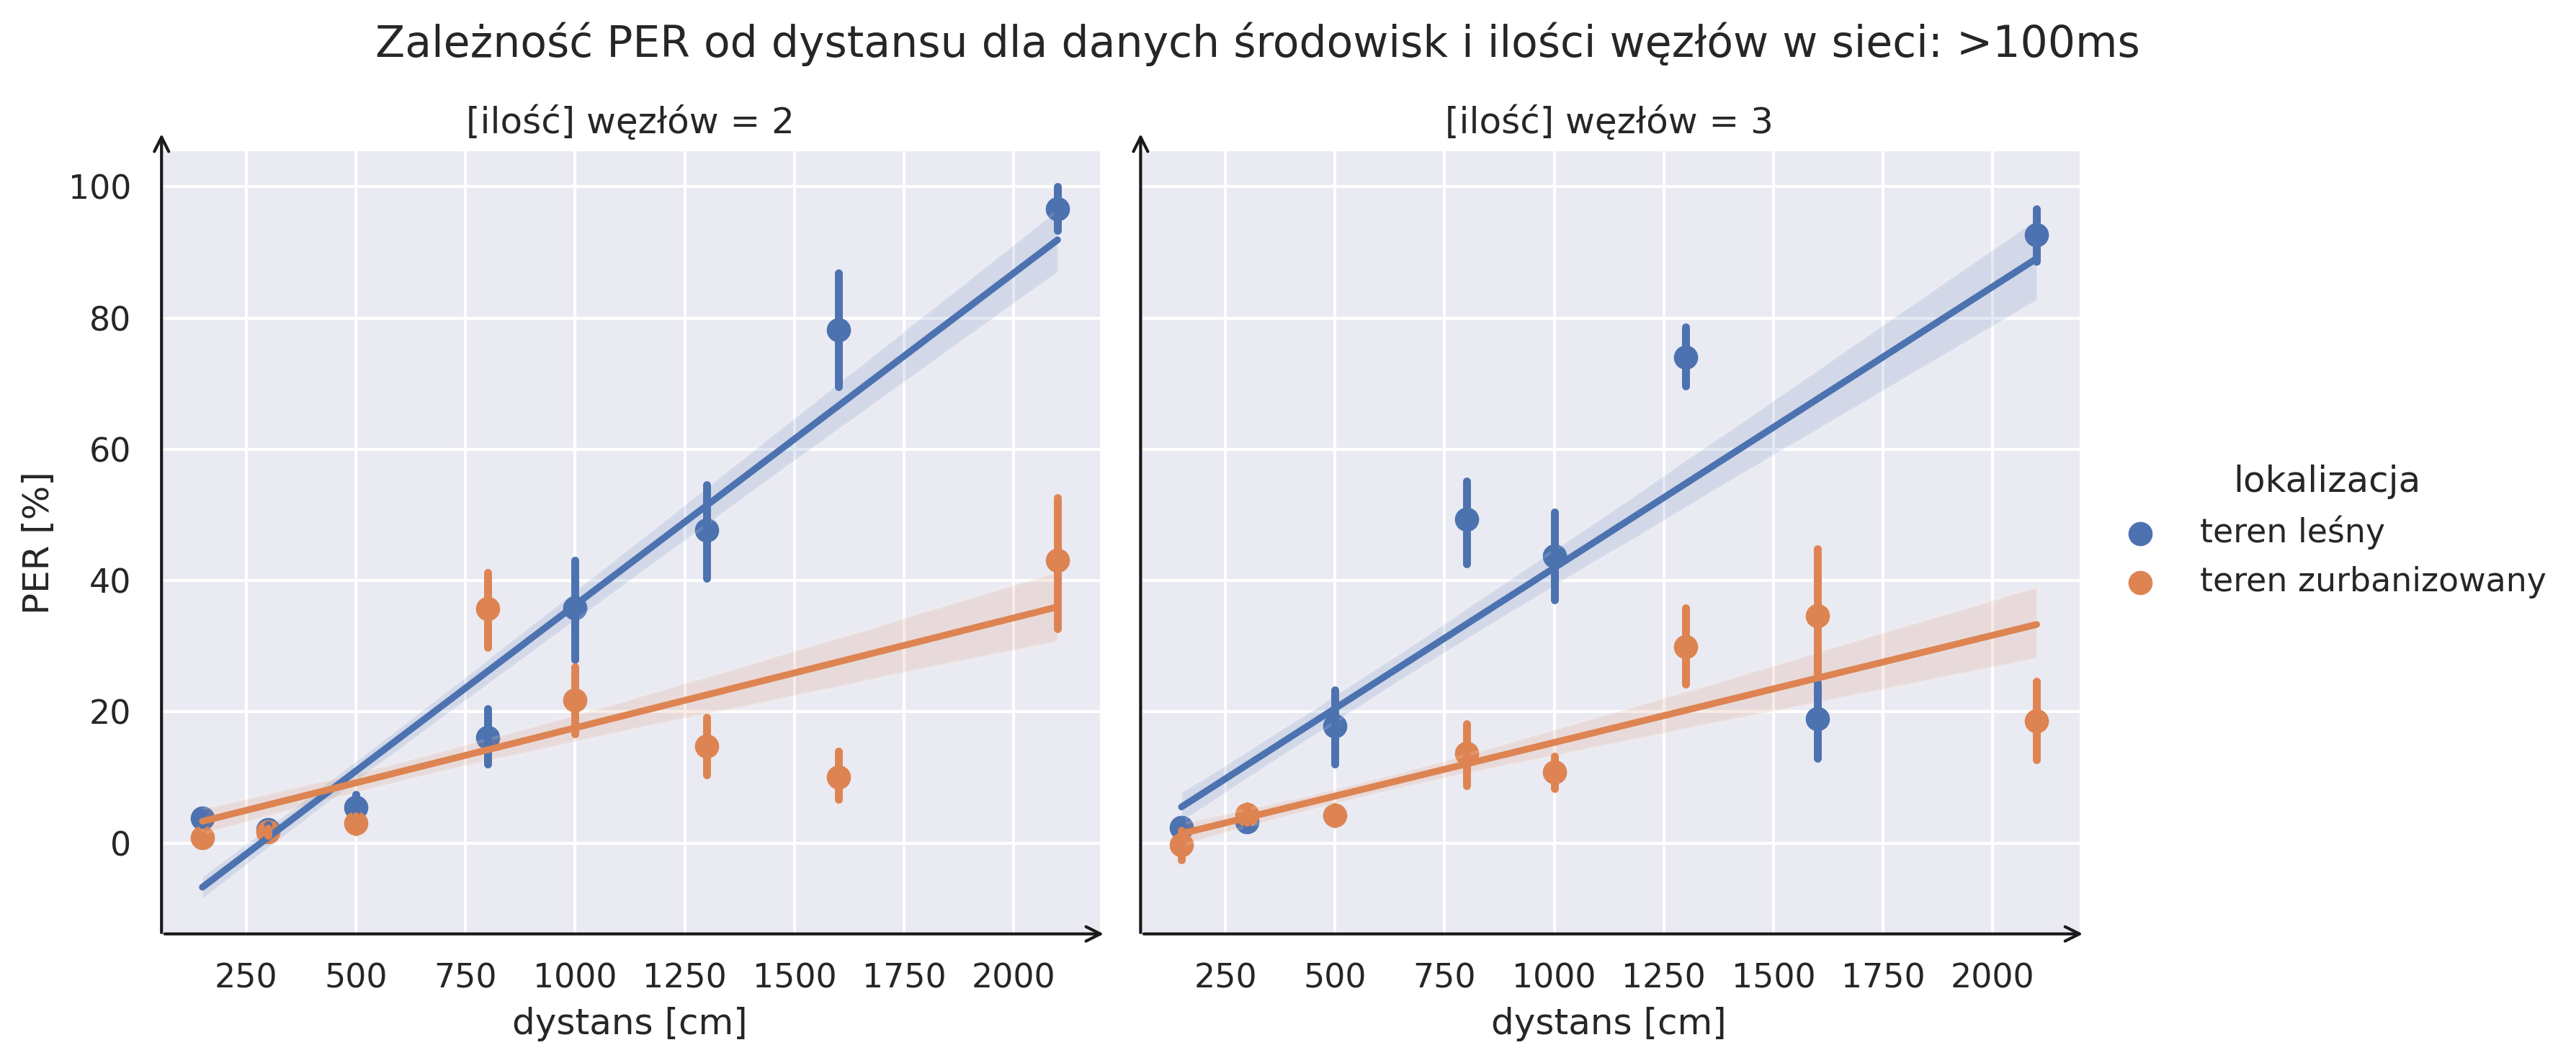
\includegraphics[width=0.99\linewidth]{per_to_distance_over_100ms_different_envs_and_nodes.png}
	\caption{Zależność \gls{PER} od dystansu dla zapytań o częstości >100ms w wybranych środowiskach i liczbę badanych węzłów}
	\label{rys:per_to_distance_over_100ms_different_envs_and_nodes}
\end{figure}





\chapter{Podsumowanie}
\label{ch:podsumowanie}
Niniejsza praca zrealizowała postawione założenia zdefiniowane we wstępie -- rozdział~\ref{ch:intro}.
Wprowadziwszy definicję sygnału płynnie wprowadzono zagadnienia związane z~rozpatrywanymi
standardami komunikacji bezprzewodowej.

Zestawiając wprowadzone protokoły, na szczególną uwagę zasługują dwa z nich: badany Bluetooth~5
(z~wyróżnieniem Mesh) oraz Thread. Opierając się na wiedzy pochodzącej z~powszechnie
dostępnej literatury, Thread osiągnął znacząco \textit{lepsze} parametry transmisji danych.
Korzyść ta rozumiana jest jako najwyższa przepustowość dla pofragmentowanych danych (Rysunek~\ref{rys:throughput_vs_hops_an1142})
oraz najmniejsze opóźnienia niezależnie od wielkości wiadomości (Rysunek~\ref{rys:latency_vs_payload_an1142}) spośród
testowanych rozwiązań.

Thread nie definiuje warstwy aplikacji, jak to umożliwiają bądź wymuszają pozostałe rozważane standardy.
Czyni to protokół uniwersalnym, niemalże ogólnego przeznaczenia, niczym protokoły TCP/IP. Porównanie jest
również nie bez znaczenia, gdyż Thread opiera się właśnie na IPv6, co znów zmniejsza nachylenie
krzywej uczenia się tego standardu i umożliwia niemalże bezpośrednio wpięcie do Internetu i~rozwiązań opartych
o~publiczną chmurę obliczeniową. Protokół ten, będąc oparty o IEEE 802.15.4, nie jest energooszczędny
do tego stopnia, co protokół BLE (Rysunek~\ref{rys:energy_per_packet_dbm_10.4108}). 
Nie czyni go to jednak gorszym a raczej przypisuje go do innych
zastosowań. Potencjalne problemy może stwarzać niewielka popularność tego protokołu wśród oferowanych
na rynku produktów. Jest to niemniej powiązane ze względnie nową architekturą danej specyfikacji.
Utrudnieniem, które bezpośrednio wpływa na kompatybilność produktów różnych producentów, jest brak
wprost zdefiniowanej warstwy aplikacji. To wyzwanie adresują projekty, takie jak 
Matter\footnote{\url{https://csa-iot.org/all-solutions/matter/}}
udostępniając specyfikację integrującą rozwiązania oparte o~Thread.

Bluetooth Mesh, pomimo rezultatów wywodzących się z~powszechnej literatury, również spełnia 
zdefiniowane przed nim standardem zadania. Protokół kładzie szczególny nacisk na organizację
i~hierarchię transmitowanych wiadomości w~warstwie. Można wystosować wręcz opinię, że został stworzony
do wysyłania \textit{tylko jednego} komunikatu, by wykonać konkretną akcję. Takie twierdzenie można
poprzeć zarówno sposobem routingu i wspomnianej hierarchii wiadomości (modele Mesh), ale również
biorąc uwagę wyniki reprezentowane na Rysunku~\ref{rys:latency_vs_payload_an1142}. Pojedynczy wysłany
komunikat cechuje się nie gorszym opóźnieniem niż pozostałe badane protokoły. Uwzględniając energooszczędność
tego standardu, czyni go nadzwyczaj interesującą opcją dla konkretnych zastosowań, np. inteligentnego
oświetlenia.

Dalsza część pracy to ćwiczenie praktyczne polegające na pomiarze zużycia energii. Zaprezentowano
charakterystyki poboru prądu w czasie dla różnych trybów funkcjonowania urządzenia dla dwóch różnych firmware'ów.
Pierwszy rozważany przypadek oparty o~BLE~\gls{HRT} jest zgodny z~przeprowadzoną symulacją -- 
Rysunki~\ref{rys:cube_pcc_advertising_1ms} oraz~\ref{rys:cube_pcc_connected_master}. Wykonana zgrubna symulacja,
bazująca na domyślnych parametrach wskazywanych przez dokumentację,
wskazywała na średni pobór prądu elektrycznego na poziomie 2,95mA (moc: 9,8mW)~\cite{noauthor_um1718_2022}. Jest to co prawda niemal
5-krotna różnica względem uzyskanych pomiarów -- maksymalny pobór prądu 0,69mA (moc: 2,27mW) -- jest ona jednak na korzyść
eksperymentu. Sugeruje to błąd dokonanych nastawów symulatora. Dopracowanie tych ustawień może stanowić kontynuację
badań tego zagadnienia. Dopracowanie tych ustawień może stanowić kontynuację

Przypadek zużycia Mesh wskazuje na zużycie energii węzła klasycznego serwera \textit{Generic OnOff}. Węzeł tego
najczęściej włączony jest do stałego źródła zasilania. Stąd, porównanie z Rysunku~\ref{rys:power_ble_consumption_comparison},
sugeruje na konieczność porównywania BLE do węzła typu \textit{LPN}, który w zamyśle -- potwierdzonym z~oficjalną specyfikacją
-- funkcjonuje z~wykorzystaniem zasilania bateryjnego. Słusznym rozwinięciem tego badania jest wykorzystania
\textit{LPN} z~jednosekundowym odświeżaniem swojego stanu (zakładając model \textit{Sensors}). Energooszczędność
BLE i Bluetooth Mesh wprost wynika z optymalizacji wykorzystania radia, co udowadnia choćby porównanie
wyników zaprezentowanych na charakterystykach~\ref{rys:power_ble_hr_fastadv_only_amps} oraz~\ref{rys:power_ble_hr_low_power_adv_only_amps},
gdzie podczas rozgłaszania niskomocowego (zgodnie z~opisywanymi w~danym rozdziale założeniami), radio przez większość
czasu nie funkcjonuje.

Eksperyment PER wskazuje na kilka interesujących zależności. Pierwszą z nich jest wydajność stosu \gls{BT} mikrokontrolera \texttt{STM32WB55RG}.
Przed przystąpieniem do formalnego doświadczenia, przeprowadzono szereg prób z~częstościami wykonywanych zapytań
znacząco mniejszymi od 100ms --~w~analogii do ciągu Fibonacciego testowano interwały 10, 20, 30, 50 i~80ms. Każdy z~nich wykazywał
tę samą cechę utraty pakietów, jak na przedstawionym Rysunku~\ref{rys:per_to_distance_under_100ms}. Przeważnie,
po kilku-kilkunastu sekundach pracy węzeł bliższy nie odpowiadał na jakiekolwiek komunikaty AT. Po ponownym uruchomieniu tego urządzenia,
działało bez zarzutu umożliwiając pobranie informacji o~odebranej liczbie pakietów z~węzła dystalnego.
Sugeruje to raczej problemy ze stosem i~ewentualnym wyciekiem pamięci uniemożliwiające poprawne funkcjonowanie sprzętu.
Jednym z~kroków do dalszych analiz jest weryfikacja kodu i~jego działania w czasie rzeczywistym. Narzędzia jakie debugger
czy valgrind\footnote{\url{https://valgrind.org/}} byłyby pierwszym krokiem ku weryfikacji zagadnienia.

Ostatnią, aczkolwiek najistotniejszą zbadaną zależnością, jest wpływ dystansu na \gls{PER}. Zgodnie ze zdefiniowaną
hipotezą w~punkcie~\ref{subsec:per_experiment} i~opisywaną później metodologią, oczekiwano dominującą rolę otaczającego
środowiska radiowego w~przeprowadzanym doświadczeniu. Projektując eksperyment nie założono znaczącego wpływu środowiska,
ani wpływu rozchodzenia się fal powierzchniowych. Zgodnie z~założeniami zaobserwowano spadek PER wraz ze wzrostem odległości.
Nie obserwuje się jednak znaczącego wpływu zależności ilości węzłów na PER.
Rysunek~\ref{rys:per_to_distance_over_100ms_different_envs_and_nodes} prezentuje PER w~postaci aproksymacji liniowej, gdzie porównywane
rezultaty dla danego środowiska od ilości węzłów są zbliżone. W punktach pomiarowych (teren zurbanizowany) 13m i~16m równoodlegle,
widać znaczny spadek PER dla dwóch węzłów, gdzie w~przypadku trzech węzłów tendencja ta jest nadal wzrostowa. Dopiero na maksymalnym
dystansie pomiarowym uwidacznia się ok. 20\% PER dla konfiguracji 3-ech urządzeń -- mniejszy niż dla 2-óch urządzeń.

Rezultaty są nieprzekonywujące. Wpływ wilgotności i~temperatury dla propagacji sygnału omawia praca~\cite{yi_lim_review_2020}.
Wilgotność ma negatywną korelację względem siły sygnału. Tłumaczone jest stratami wynikłymi z absorpcji energii sygnału. Wymieniona zależność
najprawdopodobniej uwidacznia się dla badania w~terenie leśnym. Dodatkowo, wahania w~PER na różnych dystansach przy środowisku zurbanizowanym
może sugerować nierówności terenu, czyli przeszkodę z punktu widzenia sygnału. Ten czynnik również nie został formalnie uwzględniony.

Podsumowując badanie PER, zauważa się wpływ odległości pomiędzy węzłami na wzrost wartości PER. 
Zawarty w~hipotezie badania wpływ tła radiowego (i wynikające z niego interferencja i~osłabianie fali) jest pomijalnie
mały lub czynniki trzecie w~postaci wilgotności i~nierówności terenu uniemożliwiają klarowną identyfikację tego zjawiska.

Poza wymienionymi już możliwościami dalszego rozwoju badań, sugeruje się kolejne, następujące. Uwzględniając fakt utraty pakietów
ze względu na krótki interwał odpytywań, oczywistym jest wyszukanie punktu granicznego, w którym omawiana zależność nie występuje.
Celem by było wyznaczenie minimalnego interwału, który nie powoduje utraty pakietów na niewielkich odległościach w~kontrolowanych
warunkach radiowych i~środowiskowych.

Badanie PER można dodatkowo rozwinąć uwzględniając czynniki takie jak wilgotność i~temperatura otoczenia oraz wpływ
fali powierzchniowej na transmisję sygnału. Oznacza to konieczność wykonania pomiarów w~zbliżonych, mierzalnych warunkach.
Wpływ fali powierzchniowej można zminimalizować poprzez umieszczenie węzłów na czas badań na odpowiednio wysokim statywie.
Służy to eliminacji przeszkód ze strefy Fresnela dla danych urządzeń nadawczo-odbiorczych.



    % Bibliografia - musi być
    % Bibliography - must exist
    \bibliografia

    % Strony końcowe - można zakomentować, jeśli zbędne
    % Additional pages - comment out if not needed
    
    % Wykaz symboli i skrótów - patrz opis w tekście przykładowym
    \acronymslist
    % Spis rysunków
    \listoffigures
    % Spis tabel
    \listoftables
    % Załączniki (plik appendices.tex)
    \easyappendices
\end{document}
%%%%%%%%%%%%%%%%%%%%%%%%%%%%%%%%%%%%%%%%%%%%%%%%%%%%%%%%%%%%%%%%%%%%%%%%%%%

